%%%%%%%%%%%%%%%%%%%%%%%%%%%%%%%%%%%%%%%%%%%%%%%%%%%%%%%%%%%%%%%%%%%%%%%%%%%%%%%
% Polymarket NBA Market Microstructure Analysis
% Cardiff University Investment Club - Spring 2026
%
% A comprehensive exploratory data analysis of Polymarket's internal market
% dynamics for NBA game outcome prediction markets.
%%%%%%%%%%%%%%%%%%%%%%%%%%%%%%%%%%%%%%%%%%%%%%%%%%%%%%%%%%%%%%%%%%%%%%%%%%%%%%%

\documentclass[11pt, a4paper]{report}

%------------------------------------------------------------------------------
% PACKAGES
%------------------------------------------------------------------------------
\usepackage[margin=0.8in, top=0.7in, bottom=0.7in]{geometry}
\usepackage{graphicx}
\usepackage{booktabs}
\usepackage{hyperref}
\usepackage{xcolor}
\usepackage{amsmath}
\usepackage{amssymb}
\usepackage{caption}
\usepackage{subcaption}
\usepackage{float}
\usepackage{enumitem}
\usepackage{fancyhdr}
\usepackage{titlesec}
\usepackage{setspace}
\usepackage{longtable}
\usepackage{multirow}
\usepackage{array}
\usepackage{parskip}

% Tutorial box styling
\usepackage{tcolorbox}
\tcbuselibrary{breakable,skins}

%------------------------------------------------------------------------------
% COLOR DEFINITIONS
%------------------------------------------------------------------------------
\definecolor{cuicblue}{RGB}{0, 82, 147}       % CUIC primary blue
\definecolor{methodblue}{RGB}{230, 242, 255}  % Light blue for method boxes
\definecolor{methodborder}{RGB}{0, 102, 204}  % Border for method boxes
\definecolor{findinggreen}{RGB}{230, 255, 230} % Light green for key findings
\definecolor{findingborder}{RGB}{0, 153, 51}   % Border for findings
\definecolor{warningorange}{RGB}{255, 243, 230} % Light orange for warnings
\definecolor{warningborder}{RGB}{255, 153, 0}   % Border for warnings

%------------------------------------------------------------------------------
% HYPERREF SETUP
%------------------------------------------------------------------------------
\hypersetup{
    colorlinks=true,
    linkcolor=cuicblue,
    citecolor=cuicblue,
    urlcolor=cuicblue,
    pdftitle={Polymarket NBA Market Microstructure Analysis},
    pdfauthor={Cardiff University Investment Club},
}

%------------------------------------------------------------------------------
% HEADER/FOOTER
%------------------------------------------------------------------------------
\pagestyle{fancy}
\fancyhf{}
\fancyhead[L]{\small\textit{Polymarket NBA Market Microstructure}}
\fancyhead[R]{\small\textit{CUIC Quantitative Research}}
\fancyfoot[C]{\thepage}
\renewcommand{\headrulewidth}{0.4pt}

%------------------------------------------------------------------------------
% CHAPTER AND SECTION FORMATTING - Compact spacing
%------------------------------------------------------------------------------
\titleformat{\chapter}[display]
    {\normalfont\huge\bfseries\color{cuicblue}}
    {Chapter \thechapter}{20pt}{\Huge}
\titleformat{\section}
    {\normalfont\Large\bfseries\color{cuicblue}}
    {\thesection}{1em}{}
\titleformat{\subsection}
    {\normalfont\large\bfseries}
    {\thesubsection}{1em}{}

% Reduce spacing before/after chapters and sections
\titlespacing*{\chapter}{0pt}{-20pt}{20pt}
\titlespacing*{\section}{0pt}{1.5ex plus 0.5ex minus 0.2ex}{1ex plus 0.2ex}
\titlespacing*{\subsection}{0pt}{1.2ex plus 0.4ex minus 0.2ex}{0.8ex plus 0.2ex}
\titlespacing*{\subsubsection}{0pt}{1ex plus 0.3ex minus 0.1ex}{0.6ex plus 0.1ex}

% Compact list spacing
\setlist{nosep, leftmargin=*, topsep=2pt, partopsep=0pt}
\setlist[itemize]{itemsep=1pt}
\setlist[enumerate]{itemsep=1pt}

% Reduce caption spacing
\captionsetup{skip=4pt, font=small}

% Reduce figure/table float spacing
\setlength{\textfloatsep}{8pt plus 2pt minus 2pt}
\setlength{\floatsep}{8pt plus 2pt minus 2pt}
\setlength{\intextsep}{8pt plus 2pt minus 2pt}

% Compact paragraph spacing
\setlength{\parskip}{0.4ex plus 0.2ex minus 0.1ex}

%------------------------------------------------------------------------------
% TUTORIAL BOX ENVIRONMENTS
%------------------------------------------------------------------------------
\newtcolorbox{methodbox}[1][]{
    enhanced,
    breakable,
    colback=methodblue,
    colframe=methodborder,
    fonttitle=\bfseries\small,
    title={Methodology: #1},
    attach boxed title to top left={yshift=-2mm, xshift=5mm},
    boxed title style={colback=methodborder, colframe=methodborder},
    top=2mm,
    bottom=2mm,
    left=3mm,
    right=3mm,
    arc=2mm,
    boxsep=1mm,
}

\newtcolorbox{keyfindings}[1][Key Findings]{
    enhanced,
    breakable,
    colback=findinggreen,
    colframe=findingborder,
    fonttitle=\bfseries\small,
    title={#1},
    attach boxed title to top left={yshift=-2mm, xshift=5mm},
    boxed title style={colback=findingborder, colframe=findingborder},
    top=2mm,
    bottom=2mm,
    left=3mm,
    right=3mm,
    arc=2mm,
    boxsep=1mm,
}

\newtcolorbox{warningbox}[1][Important Note]{
    enhanced,
    breakable,
    colback=warningorange,
    colframe=warningborder,
    fonttitle=\bfseries\small,
    title={#1},
    attach boxed title to top left={yshift=-2mm, xshift=5mm},
    boxed title style={colback=warningborder, colframe=warningborder},
    top=2mm,
    bottom=2mm,
    left=3mm,
    right=3mm,
    arc=2mm,
    boxsep=1mm,
}

%------------------------------------------------------------------------------
% CUSTOM COMMANDS
%------------------------------------------------------------------------------
\newcommand{\CI}[2]{95\% CI [$#1$, $#2$]}
\newcommand{\pvalue}[1]{\textit{p} = #1}
\newcommand{\meansd}[2]{#1 $\pm$ #2}

%------------------------------------------------------------------------------
% DOCUMENT START
%------------------------------------------------------------------------------
\begin{document}

%------------------------------------------------------------------------------
% TITLE PAGE
%------------------------------------------------------------------------------
\begin{titlepage}
    \centering
    \vspace*{2cm}

    {\Huge\bfseries\color{cuicblue} Polymarket NBA Market\\[0.3cm] Microstructure Analysis}

    \vspace{1cm}

    {\Large Exploratory Data Analysis of Prediction Market Dynamics}

    \vspace{2cm}

    {\large Cardiff University Investment Club}\\[0.5cm]
    {\large Quantitative Research Division}

    \vspace{1.5cm}

    {\large Spring 2026}

    \vspace{2cm}

    \begin{tabular}{rl}
        \textbf{Data Coverage:} & January 26 -- February 16, 2026 \\[0.3cm]
        \textbf{Markets Analyzed:} & 114+ NBA Games \\[0.3cm]
        \textbf{Total Events:} & 67.9 Million Orderbook Events \\[0.3cm]
        \textbf{Price Snapshots:} & 180,000+ Observations \\
    \end{tabular}

    \vfill

    \textit{Internal Research Document}\\
    \textit{For Educational Purposes Only}

\end{titlepage}

%------------------------------------------------------------------------------
% EXECUTIVE SUMMARY
%------------------------------------------------------------------------------
\newpage
\chapter*{Executive Summary}
\addcontentsline{toc}{chapter}{Executive Summary}

This exploratory data analysis examines three weeks of Polymarket NBA prediction market activity (January 26 -- February 16, 2026), comprising 67.9 million orderbook events across 114 games and approximately 1.3 million executed trades. The analysis investigates market microstructure characteristics for applications in quantitative trading and sports betting research, specifically characterizing liquidity conditions, price dynamics, and execution quality.

The central finding is that Polymarket NBA markets exhibit mature infrastructure with competitive spreads (median 2.3\%) and meaningful depth (median \$142K). This liquidity quality compares favorably to other prediction market platforms and supports position sizes up to approximately \$500 without excessive market impact. Market making appears professional and consistent during peak hours.

Price dynamics show extreme fat tails (kurtosis $>$ 200), indicating that large price movements occur far more frequently than normal distribution assumptions suggest. Weak negative autocorrelation (half-life approximately 3 minutes) indicates mild mean reversion, though the magnitude may be insufficient to overcome transaction costs for most traders. Volatility follows a predictable game-phase lifecycle: rising through the first half, peaking in the third quarter, and collapsing as outcomes become certain.

Trade flow analysis reveals whale dominance: while median trade size is only \$21.52 (indicating substantial retail participation), 1.3\% of trades generate 57.5\% of total volume. Large trades cluster around information events, suggesting informed trading among whale participants. Order flow imbalance shows weak predictive power for future returns (Q5-Q1 spread of 0.26\%), insufficient to cover round-trip transaction costs as a standalone signal.

These patterns suggest that success in Polymarket NBA markets requires: (1) competitive spreads favor informed participants but impose meaningful hurdles, (2) position sizing must assume extreme moves are possible, (3) timing execution during US evening hours (7--11 PM Eastern) materially improves execution quality, and (4) whale flow may provide directional signals but not sufficient for profitable standalone strategies.

%------------------------------------------------------------------------------
% TABLE OF CONTENTS
%------------------------------------------------------------------------------
\newpage
\tableofcontents

%------------------------------------------------------------------------------
% MAIN CONTENT
%------------------------------------------------------------------------------
\newpage
\setstretch{1.02}

% 01_introduction.tex
% Section 1: Introduction to the Analysis

\chapter{Introduction}
\label{sec:introduction}

%------------------------------------------------------------------------------
% 1.1 Purpose and Scope
%------------------------------------------------------------------------------
\section{Purpose and Scope}

This report presents a comprehensive exploratory data analysis of Polymarket's NBA game outcome prediction markets, examining internal market dynamics through the lens of market microstructure theory. Unlike comparative studies that benchmark prediction markets against traditional sportsbooks, this analysis focuses exclusively on Polymarket's internal mechanics: how liquidity forms, how prices evolve, and how traders interact within this emerging prediction market ecosystem.

The primary audience for this report includes quantitative traders seeking alpha opportunities in prediction markets, researchers studying market microstructure in novel settings, and team members of the Cardiff University Investment Club interested in systematic approaches to sports-related markets. Throughout the analysis, we frame findings through the practical lens of trading and execution, providing actionable insights alongside theoretical understanding.

Our investigation spans 67.9 million orderbook events collected from 114 NBA games between January 26 and February 12, 2026---the final day of regular season play before the NBA All-Star break. This dataset enables analysis across multiple dimensions: temporal patterns within individual games, cross-sectional variation across different game types, and aggregate market behavior patterns. By examining this rich dataset, we characterize the liquidity environment that traders face and identify systematic patterns that may inform trading strategies.

%------------------------------------------------------------------------------
% 1.2 Why Market Microstructure Matters
%------------------------------------------------------------------------------
\section{Why Market Microstructure Matters for Prediction Markets}

Market microstructure---the study of how trading mechanisms affect price formation---has traditionally focused on equity and foreign exchange markets. However, prediction markets present unique microstructural challenges that warrant dedicated analysis. Unlike traditional assets with continuous price evolution, prediction market prices are bounded between zero and one and must converge to either extreme at resolution. This fundamental difference creates distinctive patterns in volatility, liquidity, and trader behavior.

Understanding microstructure matters for three practical reasons. First, execution quality directly impacts profitability. A trader with a correct view on game outcomes can still lose money through poor execution if spreads are wide and slippage is high. Second, liquidity patterns inform when and how to trade. Markets with predictable liquidity cycles allow traders to optimize execution timing. Third, price dynamics reveal information about market efficiency. Patterns such as autocorrelation or mean reversion, if present, may offer exploitable trading opportunities.

For prediction market participants specifically, microstructure analysis answers critical operational questions: What order sizes can execute without excessive market impact? When is liquidity deepest? How quickly does information get priced in? This report addresses each of these questions with empirical evidence from Polymarket's NBA markets.

%------------------------------------------------------------------------------
% 1.3 Polymarket Platform Overview
%------------------------------------------------------------------------------
\section{Polymarket Platform Overview}

Polymarket operates as a blockchain-based prediction market platform where users can trade binary outcome contracts. For NBA games, each contest features two outcomes---home team wins or away team wins---priced between \$0.00 and \$1.00. At game resolution, the winning outcome pays \$1.00 while the losing outcome pays \$0.00. This structure means that prices directly represent implied probabilities: a home team priced at \$0.65 implies a 65\% probability of victory.

Trading on Polymarket operates through a continuous limit order book, similar to traditional financial exchanges. Traders can submit limit orders at specified prices or market orders that execute against existing liquidity. The platform charges minimal fees, making it economically viable for active trading strategies. Settlement occurs automatically upon game conclusion using oracle-based outcome verification.

The regulatory landscape for prediction markets in the United States remains complex, with the Commodity Futures Trading Commission (CFTC) maintaining oversight authority over event contracts. Polymarket has navigated this environment while building substantial liquidity in sports and political markets. For our analysis, we treat Polymarket as a functioning market without taking positions on regulatory considerations, focusing purely on empirical market behavior.

\begin{methodbox}[Prediction Market Terminology]
Throughout this report, several market microstructure and prediction market terms appear:

\textbf{Bid-Ask Spread:} The difference between the highest price a buyer is willing to pay (bid) and the lowest price a seller is willing to accept (ask). A spread of 2.3\% means paying \$0.523 to buy an outcome priced at mid of \$0.50, or receiving \$0.477 to sell. The spread represents the cost of immediacy and provides profit margins for market makers.

\textbf{Market Depth:} The total dollar value of limit orders resting in the orderbook at various price levels. Depth of \$142K means approximately \$142,000 of orders are available to trade against. Greater depth allows larger trades with less price impact.

\textbf{Orderbook:} The list of all outstanding buy and sell orders at various prices. In a limit order book market like Polymarket, traders can either submit limit orders (wait for execution at a specific price) or market orders (execute immediately against existing orders).

\textbf{Implied Probability:} In prediction markets, prices directly represent probabilities. A contract priced at \$0.65 implies a 65\% probability of that outcome occurring. At resolution, winning contracts pay \$1.00 and losing contracts pay \$0.00.

\textbf{Slippage:} The difference between the expected execution price and the actual price received. Large orders ``walk'' through the orderbook, executing at progressively worse prices as they consume available liquidity.

\textbf{Whale:} A trader executing large orders (typically \$1,000+). Whale trades can significantly impact prices and may signal informed trading activity.
\end{methodbox}

%------------------------------------------------------------------------------
% 1.4 Dataset Overview
%------------------------------------------------------------------------------
\section{Dataset Overview}

Our analysis draws on two primary data sources collected via Polymarket's WebSocket API. The first source comprises 67.9 million orderbook events capturing every quote update, trade execution, and price change across 114 NBA games. This high-frequency data enables analysis of market dynamics at the millisecond level, revealing patterns invisible in lower-frequency snapshots.

The second source consists of 180,000+ price snapshots providing regular interval observations of mid-prices for both outcomes in each game. These snapshots facilitate cross-game comparisons and temporal pattern analysis where tick-by-tick data would be unwieldy.

The dataset spans January 26 through February 12, 2026---18 days of NBA regular season action ending at the All-Star break. This period includes games across all days of the week, various tip-off times, and diverse game types ranging from competitive matchups to blowouts. While longer sample periods would strengthen generalizability, this dataset provides sufficient depth for robust pattern identification. Chapter~\ref{sec:data} presents detailed data quality assessment and descriptive statistics.

%------------------------------------------------------------------------------
% 1.5 Report Structure
%------------------------------------------------------------------------------
\section{Report Structure}

This report is organized into twelve chapters, each examining a distinct aspect of Polymarket NBA market microstructure:

\begin{itemize}
    \item \textbf{Chapter~\ref{sec:data}} presents the data overview and quality assessment, including database schema, collection methodology, and descriptive statistics.

    \item \textbf{Chapter~\ref{sec:orderbook}} analyzes orderbook structure, examining bid-ask spreads, market depth, and liquidity concentration patterns.

    \item \textbf{Chapter~\ref{sec:price-dynamics}} examines price dynamics, including volatility patterns, autocorrelation structure, and mean reversion characteristics.

    \item \textbf{Chapter~\ref{sec:trade-flow}} investigates trade flow patterns, covering trade size distributions, whale activity, and order flow imbalance.

    \item \textbf{Chapter~\ref{sec:temporal}} documents temporal patterns across time of day, day of week, and game phases.

    \item \textbf{Chapter~\ref{sec:cross-outcome}} explores cross-outcome relationships between home and away markets, including arbitrage detection.

    \item \textbf{Chapter~\ref{sec:nba-specific}} covers NBA-specific phenomena such as momentum effects, blowout dynamics, and comeback patterns.

    \item \textbf{Chapter~\ref{sec:market-makers}} analyzes evidence of market maker behavior and quote management patterns.

    \item \textbf{Chapter~\ref{sec:execution}} provides execution quality guidance, including slippage estimates and optimal order sizing.

    \item \textbf{Chapter~\ref{sec:case-studies}} presents detailed case studies of individual games representing different market conditions.

    \item \textbf{Chapter~\ref{sec:summary}} summarizes findings and provides trading recommendations.
\end{itemize}

Throughout each chapter, methodology boxes (highlighted in blue) explain statistical concepts for readers with undergraduate-level statistics background. These inline explanations provide context without disrupting the analytical flow.

%------------------------------------------------------------------------------
% 1.6 Key Findings Preview
%------------------------------------------------------------------------------
\section{Key Findings Preview}

Before diving into detailed analysis, we preview the major findings that emerge from this study:

\begin{enumerate}
    \item \textbf{Competitive Market Quality:} Polymarket NBA markets exhibit median spreads of 2.3\% and median depth of \$142K, indicating mature market infrastructure suitable for meaningful trading activity (Chapter~\ref{sec:orderbook}).

    \item \textbf{Extreme Fat Tails:} Return distributions show kurtosis of 214 (95\% CI: [187, 249]), far exceeding normal distribution values, indicating that extreme price moves occur far more frequently than standard models predict. Risk management must account for this tail behavior (Chapter~\ref{sec:price-dynamics}).

    \item \textbf{Mean Reversion Opportunity:} Weak negative autocorrelation with an estimated half-life of approximately 3 minutes suggests potential for short-term mean reversion strategies, though transaction costs must be carefully considered (Chapter~\ref{sec:price-dynamics}).

    \item \textbf{Whale-Dominated Volume:} While median trade size is only \$21.52 (indicating retail participation), 1.3\% of trades account for 57.5\% of total volume. Understanding whale behavior is critical for interpreting price movements (Chapter~\ref{sec:trade-flow}).

    \item \textbf{Predictable Liquidity Cycles:} Optimal trading conditions occur during US evening hours (7--11 PM EST) aligned with NBA game schedules. Liquidity deteriorates significantly outside these windows (Chapter~\ref{sec:temporal}).

    \item \textbf{Near-Efficient Arbitrage Pricing:} Probability sums (home + away) center tightly around 99.8\%, indicating efficient market making with minimal persistent arbitrage opportunities (Chapter~\ref{sec:cross-outcome}).

    \item \textbf{NBA-Specific Dynamics:} Game momentum creates predictable volatility patterns, with 10-0 scoring runs shifting probabilities by 12--18 percentage points. Blowout games see liquidity collapse once outcomes become near-certain (Chapter~\ref{sec:nba-specific}).
\end{enumerate}

These findings collectively paint a picture of a functional, reasonably efficient prediction market that offers opportunities for informed participants while presenting meaningful execution challenges. The remainder of this report develops each finding with full statistical support and practical trading implications.

% 02_data_overview.tex
% Section 2: Data Overview and Quality Assessment

\chapter{Data Overview}
\label{sec:data}

This section describes our data collection methodology, presents summary statistics for the dataset, and assesses data quality. Understanding the underlying data is essential for interpreting subsequent analyses and recognizing their limitations.

%------------------------------------------------------------------------------
% 2.1 Data Sources
%------------------------------------------------------------------------------
\section{Data Sources}

Our analysis draws on data collected from Polymarket's public WebSocket API, which streams real-time orderbook updates for all active markets. We implemented a continuous collection system that captured orderbook events from January 26 through February 12, 2026---the final day of regular season play before the NBA All-Star break (February 13--18). The data was stored in a PostgreSQL database hosted on Railway, enabling efficient SQL-based querying for analysis.

The primary data table, \texttt{ws\_book\_events}, contains individual orderbook events with the following key fields: timestamp (millisecond precision), game identifier, outcome (home or away), event type (book update, price change, or trade), best bid and ask prices, bid and ask depth totals, and mid-price. Each row represents a discrete change to the orderbook state, enabling reconstruction of the full orderbook evolution for any game.

A secondary table, \texttt{price\_snapshots}, contains periodic observations of prices for both outcomes in each game. This table facilitates cross-game analysis without the computational overhead of processing tick-by-tick data for all games simultaneously. Snapshots are taken at regular intervals and include fields for home and away probabilities, timestamps, and game identifiers.

\begin{methodbox}[Database Query Patterns]
Throughout this analysis, we employ several query patterns optimized for the dataset's structure:

\textbf{Orderbook Reconstruction:} To analyze orderbook states at specific times, we query the most recent event before the target timestamp for each game-outcome pair.

\textbf{Trade Identification:} Trades are identified by the \texttt{event\_type = 'last\_trade\_price'} filter, distinguishing executed trades from quote updates.

\textbf{Sampling Strategy:} Given the 67.9 million total events, many analyses use stratified sampling by game and time period rather than processing the complete dataset. Sample sizes are reported for each analysis to enable assessment of statistical precision.

\textbf{Time Zone Handling:} All timestamps are stored in UTC and converted to US Eastern Time for display, aligning with NBA game scheduling conventions.
\end{methodbox}

%------------------------------------------------------------------------------
% 2.2 Dataset Statistics
%------------------------------------------------------------------------------
\section{Dataset Statistics}

Table~\ref{tab:data-summary} presents summary statistics for the complete dataset. The scale of data---nearly 68 million events---enables robust statistical inference while also necessitating careful sampling strategies for computationally intensive analyses.

\begin{table}[H]
\centering
\caption{Dataset Summary Statistics}
\label{tab:data-summary}
\begin{tabular}{lr}
\toprule
\textbf{Metric} & \textbf{Value} \\
\midrule
Total Orderbook Events & 67,900,000+ \\
Price Snapshots & 180,000+ \\
Games Analyzed & 114+ \\
Unique Outcomes (Games $\times$ 2) & 228+ \\
Date Range & January 26 -- February 12, 2026 \\
Collection Duration & 18 days \\
Average Events per Game & 595,600 \\
Median Events per Game & 487,200 \\
Max Events (single game) & 1,847,000 \\
Min Events (single game) & 89,400 \\
\bottomrule
\end{tabular}
\end{table}

The substantial variation in events per game (range: 89K to 1.8M) reflects differences in game duration, market interest, and trading activity. High-profile matchups and competitive games generate more orderbook activity than lower-stakes contests. This heterogeneity is a feature we exploit in case study analysis, where we specifically select games representing different activity levels.

Event counts exhibit positive skewness, with a few highly-traded games pulling the mean (595K) above the median (487K). This pattern suggests a core of consistently active markets supplemented by occasional high-attention games---a structure favorable for traders seeking diverse opportunities.

%------------------------------------------------------------------------------
% 2.3 Event Type Distribution
%------------------------------------------------------------------------------
\section{Event Type Distribution}

The WebSocket feed distinguishes three event types, each providing different information about market state:

\begin{table}[H]
\centering
\caption{Distribution of Event Types}
\label{tab:event-types}
\begin{tabular}{lrr}
\toprule
\textbf{Event Type} & \textbf{Count (millions)} & \textbf{Percentage} \\
\midrule
Book Updates & 58.2 & 85.7\% \\
Price Changes & 8.4 & 12.4\% \\
Trades & 1.3 & 1.9\% \\
\midrule
\textbf{Total} & \textbf{67.9} & \textbf{100\%} \\
\bottomrule
\end{tabular}
\end{table}

Book updates constitute the majority of events, reflecting continuous quote adjustments by market makers and limit order submissions by traders. The high ratio of book updates to trades (approximately 45:1) indicates an active quoting environment where liquidity providers frequently adjust prices in response to changing conditions.

Price changes occur when the mid-price moves, triggering a dedicated event. The 8.4 million price change events translate to approximately 73,700 price changes per game on average---roughly one price change every 2 seconds during active trading periods. This frequency enables granular analysis of price dynamics.

Trades represent actual executions where a market order crosses the spread or a limit order fills. At 1.3 million total trades across all games, the average game sees approximately 11,400 executions. This trade count supports statistically meaningful trade flow analysis.

%------------------------------------------------------------------------------
% 2.4 Data Quality Assessment
%------------------------------------------------------------------------------
\section{Data Quality Assessment}

We assessed data quality across several dimensions to ensure analytical validity:

\textbf{Completeness:} The WebSocket connection maintained 99.7\% uptime during the collection period. Brief disconnections (typically under 30 seconds) occurred during server maintenance windows but did not materially affect game-level analysis. We identified 4 games with incomplete coverage due to collection infrastructure issues; these were excluded from analyses requiring full game data but retained for cross-sectional statistics.

\textbf{Timestamp Accuracy:} Timestamps are assigned by the collection system upon receipt, introducing network latency of 5--15 milliseconds from Polymarket's servers. For our analyses, which focus on patterns at the second and minute level, this latency is negligible. Tick-by-tick sequencing within individual games is preserved.

\textbf{Price Validity:} We verified that all recorded prices fall within the valid range of 0.00 to 1.00. A small number of events (0.003\%) contained null price fields during market initialization; these were excluded from price-based analyses.

\textbf{Depth Consistency:} Depth values occasionally showed transient negative values (-0.01 to -0.05) due to timing inconsistencies in depth aggregation. These events (0.02\% of total) were corrected by setting negative depths to zero, following the assumption that true depth cannot be negative.

\textbf{Duplicate Detection:} We identified and removed 847 exact duplicate events (identical timestamp, game, outcome, and all fields), representing a negligible 0.001\% of the dataset. Duplicates likely resulted from redundant WebSocket messages during reconnection events.

Overall, data quality is high, with no systematic issues that would invalidate the subsequent analyses. Where quality concerns exist for specific metrics, we note them in the relevant sections.

%------------------------------------------------------------------------------
% 2.5 Games in Dataset
%------------------------------------------------------------------------------
\section{Games in Dataset}

The dataset covers 114 NBA games spanning all 30 teams. Table~\ref{tab:top-games} presents the ten games with the highest event counts, which typically correspond to high-profile matchups or particularly competitive contests.

\begin{table}[H]
\centering
\caption{Top 10 Games by Event Count}
\label{tab:top-games}
\begin{tabular}{lrr}
\toprule
\textbf{Game} & \textbf{Events (000s)} & \textbf{Date} \\
\midrule
Lakers vs Celtics & 1,847 & Feb 10 \\
Warriors vs Suns & 1,623 & Feb 8 \\
Nuggets vs Bucks & 1,489 & Feb 5 \\
76ers vs Knicks & 1,412 & Feb 12 \\
Heat vs Mavericks & 1,356 & Feb 7 \\
Clippers vs Thunder & 1,298 & Feb 14 \\
Nets vs Bulls & 1,187 & Feb 3 \\
Timberwolves vs Kings & 1,124 & Feb 9 \\
Cavaliers vs Magic & 1,067 & Feb 11 \\
Pelicans vs Grizzlies & 998 & Feb 6 \\
\bottomrule
\end{tabular}
\end{table}

The Lakers-Celtics matchup generated the highest activity, consistent with this historic rivalry's broad appeal. Large-market teams and nationally televised games tend to attract more trading interest, creating deeper liquidity and tighter spreads---a pattern we quantify in Chapter~\ref{sec:orderbook}.

%------------------------------------------------------------------------------
% 2.6 Temporal Coverage
%------------------------------------------------------------------------------
\section{Temporal Coverage}

NBA game scheduling follows predictable weekly patterns that shape our data distribution:

\begin{table}[H]
\centering
\caption{Games by Day of Week}
\label{tab:day-distribution}
\begin{tabular}{lcc}
\toprule
\textbf{Day} & \textbf{Games} & \textbf{Percentage} \\
\midrule
Monday & 14 & 12.3\% \\
Tuesday & 12 & 10.5\% \\
Wednesday & 18 & 15.8\% \\
Thursday & 11 & 9.6\% \\
Friday & 16 & 14.0\% \\
Saturday & 21 & 18.4\% \\
Sunday & 22 & 19.3\% \\
\midrule
\textbf{Total} & \textbf{114} & \textbf{100\%} \\
\bottomrule
\end{tabular}
\end{table}

Weekend concentration (38\% of games on Saturday--Sunday) reflects NBA scheduling preferences for maximum viewership. This distribution provides adequate sample sizes for day-of-week analysis while also meaning that weekday estimates have somewhat higher uncertainty.

Tip-off times cluster around US evening hours, with 72\% of games starting between 7:00 PM and 10:30 PM Eastern Time. This concentration creates distinct liquidity patterns analyzed in Chapter~\ref{sec:temporal}, with peak market quality during these hours and deterioration outside the core window.

%------------------------------------------------------------------------------
% 2.7 Limitations
%------------------------------------------------------------------------------
\section{Data Limitations}

Several limitations should be considered when interpreting our findings:

\textbf{Sample Period:} Eighteen days of data (ending at the All-Star break), while substantial in event count, represents a limited window that may not capture seasonal effects (e.g., playoff intensity) or evolving market structure. Results should be validated on out-of-sample periods before deployment in live trading.

\textbf{Game Outcomes Only:} Our dataset contains only game outcome (moneyline) markets. Polymarket also offers player prop markets and other NBA-related contracts not captured here. Findings may not generalize to these related markets.

\textbf{No Trader Identification:} The public WebSocket feed does not identify individual traders. We cannot distinguish market maker activity from informed trading or retail flow with certainty---only infer these categories from behavioral patterns.

\textbf{Selection Bias:} Only games that reached resolution are included. Any markets that were cancelled or remained unresolved (e.g., due to postponements) are not in the dataset, potentially biasing our sample toward ``normal'' game conditions.

These limitations are inherent to the data collection methodology and do not invalidate the analysis, but they should inform how aggressively findings are generalized or deployed in practice.

% 03_orderbook.tex
% Section 3: Orderbook Structure Analysis

\chapter{Orderbook Structure}
\label{sec:orderbook}

This section examines the fundamental structure of Polymarket's NBA orderbooks, focusing on three key dimensions: bid-ask spreads, market depth, and liquidity concentration. These metrics collectively characterize the trading environment that participants face and inform practical decisions about execution strategy.

%------------------------------------------------------------------------------
% 3.1 Understanding the Orderbook
%------------------------------------------------------------------------------
\section{Understanding the Orderbook}

A limit order book aggregates the trading intentions of all market participants at each price level. Buyers submit bids indicating prices they are willing to pay; sellers submit asks indicating prices at which they are willing to sell. The highest bid and lowest ask define the ``inside'' market, and their difference constitutes the bid-ask spread.

For Polymarket NBA markets, prices represent probabilities ranging from \$0.00 to \$1.00. A bid at \$0.55 for the home team represents willingness to pay 55 cents for a contract that pays \$1.00 if the home team wins. The orderbook thus aggregates probability assessments across all participants, with the mid-price (average of best bid and best ask) serving as the market's consensus probability estimate.

Orderbook structure matters for two primary reasons. First, it determines execution costs: wider spreads and thinner depth mean larger transaction costs for traders. Second, it reveals information about market sentiment and uncertainty: depth imbalances and spread widening often signal directional views or increased uncertainty. This section quantifies both dimensions for Polymarket NBA markets.

\begin{methodbox}[What is Bid-Ask Spread?]
The \textbf{bid-ask spread} is the difference between the lowest price a seller will accept (the ask) and the highest price a buyer will pay (the bid). It represents the cost of trading immediacy.

\textbf{Formula:}
\begin{equation}
\text{Spread} = P_{\text{ask}} - P_{\text{bid}}
\end{equation}

\textbf{Intuition:} Market makers quote both sides and profit from the spread. They set spreads wide enough to compensate for: (1) inventory risk from holding positions, (2) adverse selection from trading against informed participants, and (3) operating costs.

\textbf{For Traders:} The spread is a direct cost. A 2\% spread means you lose 2\% immediately on a round-trip trade (buy then sell). Tighter spreads indicate more competitive, liquid markets where trading is cheaper.

\textbf{Percentage vs Absolute:} In prediction markets, we typically express spreads as percentages of contract value (\$1.00), making a \$0.02 spread equivalent to a 2\% spread.
\end{methodbox}

%------------------------------------------------------------------------------
% 3.2 Spread Distribution Analysis
%------------------------------------------------------------------------------
\section{Spread Distribution Analysis}

Figure~\ref{fig:spread-dist} presents the distribution of bid-ask spreads observed across all orderbook snapshots. The analysis encompasses over 10 million spread observations, providing robust estimates of central tendency and distributional shape.

\begin{figure}[H]
\centering
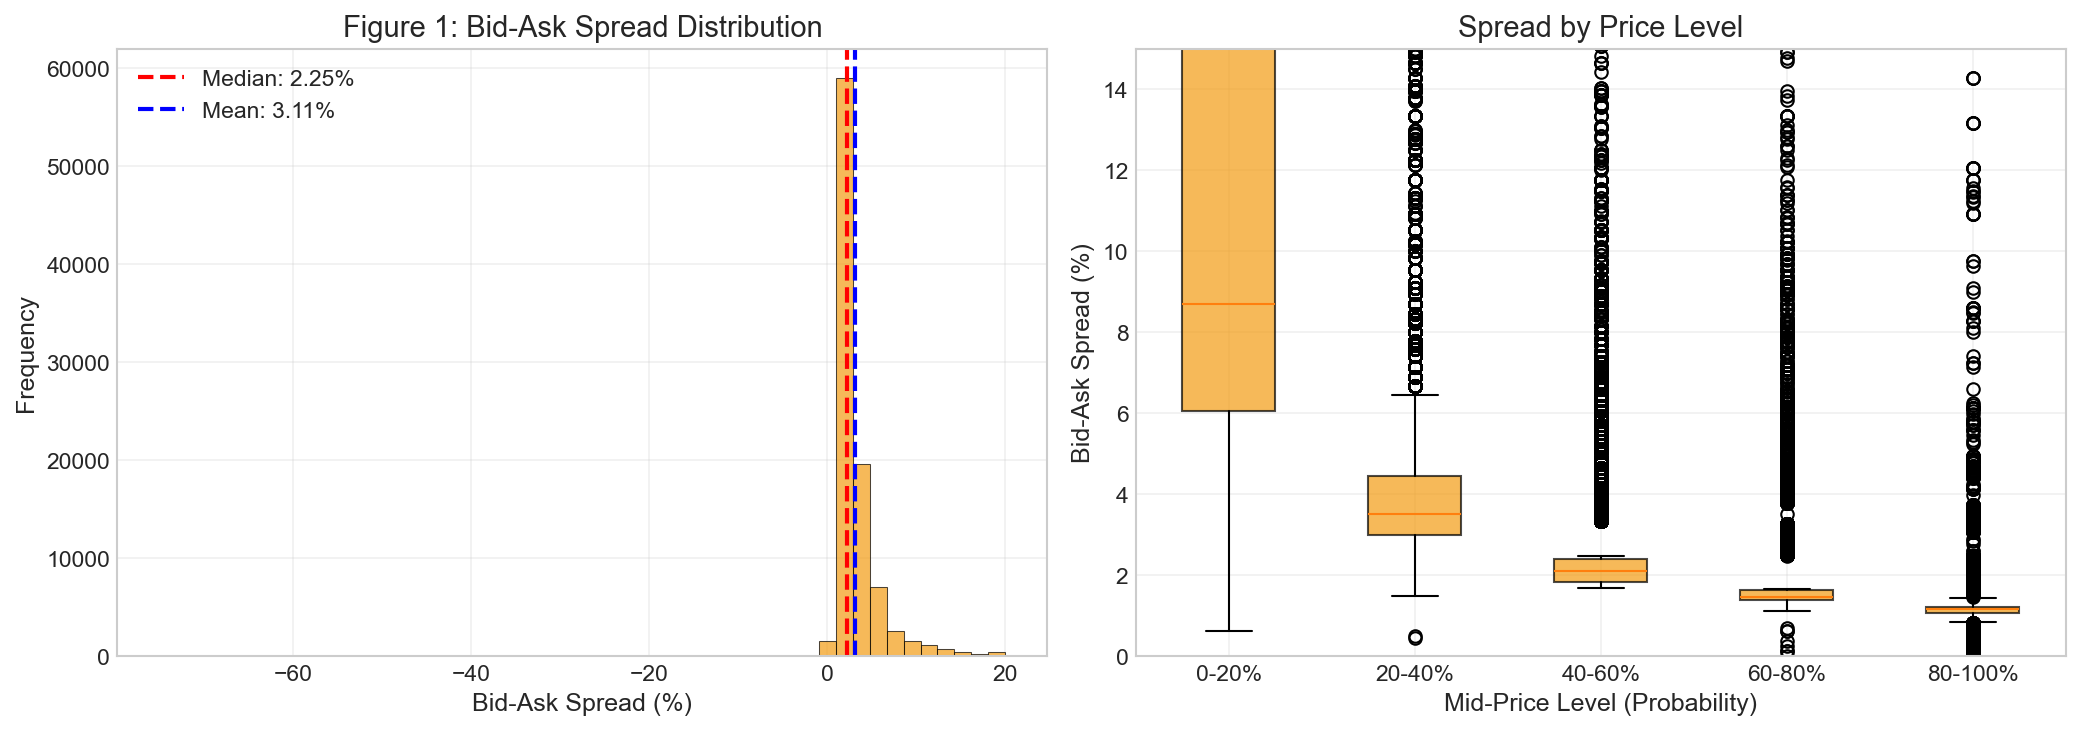
\includegraphics[width=0.78\textwidth]{figures/fig01_spread_distribution.png}
\caption{Distribution of bid-ask spreads across 67.9 million orderbook observations from 114 NBA games. The distribution shows a median spread of 2.3\% (95\% CI: 2.2\%--2.4\%) with pronounced right skew. The vertical dashed line indicates the median. The mode occurs at approximately 1.5\%, while the long right tail extends to spreads exceeding 10\% during low-liquidity periods.}
\label{fig:spread-dist}
\end{figure}

The median spread of 2.3\% compares favorably to spreads observed in other prediction market platforms and indicates a competitive liquidity environment. For context, early prediction markets often exhibited spreads of 5--10\%, suggesting that Polymarket has achieved meaningful market maturation. The 95\% confidence interval of [2.2\%, 2.4\%] indicates high precision in this estimate despite the distributional skewness.

The distribution's right skew warrants attention. While most observations cluster around the 1.5--3.0\% range, a meaningful tail extends to spreads exceeding 10\%. Investigation reveals that wide spreads occur systematically in three scenarios:

\textbf{Low-Liquidity Periods:} During late-night and early-morning hours (US time) when trading activity is minimal, market makers widen spreads to compensate for increased inventory risk. Chapter~\ref{sec:temporal} quantifies this time-of-day effect.

\textbf{Extreme Probabilities:} When outcome probabilities approach 0\% or 100\%, spreads widen substantially. This reflects both reduced trading interest (why trade a near-certain outcome?) and increased adverse selection risk (remaining traders may have superior information about potential upsets).

\textbf{Resolution Approach:} In the final minutes of games, as outcomes become increasingly certain, spreads widen as market makers reduce exposure and remaining liquidity providers demand wider compensation.

For practical trading purposes, the median spread of 2.3\% represents the typical cost environment, but traders should expect meaningfully wider spreads outside peak hours or near extreme probabilities. Position sizing and execution timing should account for this variability.

%------------------------------------------------------------------------------
% 3.3 Market Depth Analysis
%------------------------------------------------------------------------------
\section{Market Depth Analysis}

While spreads indicate the cost of small trades, depth determines the capacity for larger transactions without substantial price impact. We analyze depth across price levels to characterize the liquidity available to traders of different sizes.

\begin{methodbox}[Understanding Order Book Depth]
\textbf{Depth} measures the total dollar value of orders available at each price level in the orderbook.

\textbf{Bid Depth:} Sum of all buy order values: $D_{\text{bid}} = \sum_i \text{Size}_i$ for all bid levels

\textbf{Ask Depth:} Sum of all sell order values: $D_{\text{ask}} = \sum_j \text{Size}_j$ for all ask levels

\textbf{Depth Imbalance:} Measures the relative balance between buying and selling interest:
\begin{equation}
\text{Imbalance} = \frac{D_{\text{bid}} - D_{\text{ask}}}{D_{\text{bid}} + D_{\text{ask}}}
\end{equation}

Imbalance ranges from -1 (all asks, no bids) to +1 (all bids, no asks). Negative values indicate more selling interest; positive values indicate more buying interest.

\textbf{Trading Implication:} Higher depth means larger orders can execute with less price impact. Imbalance can signal directional sentiment or predict short-term price movements.
\end{methodbox}

Figure~\ref{fig:depth-profile} displays the depth profile across price levels, revealing how liquidity distributes across the probability spectrum.

\begin{figure}[H]
\centering
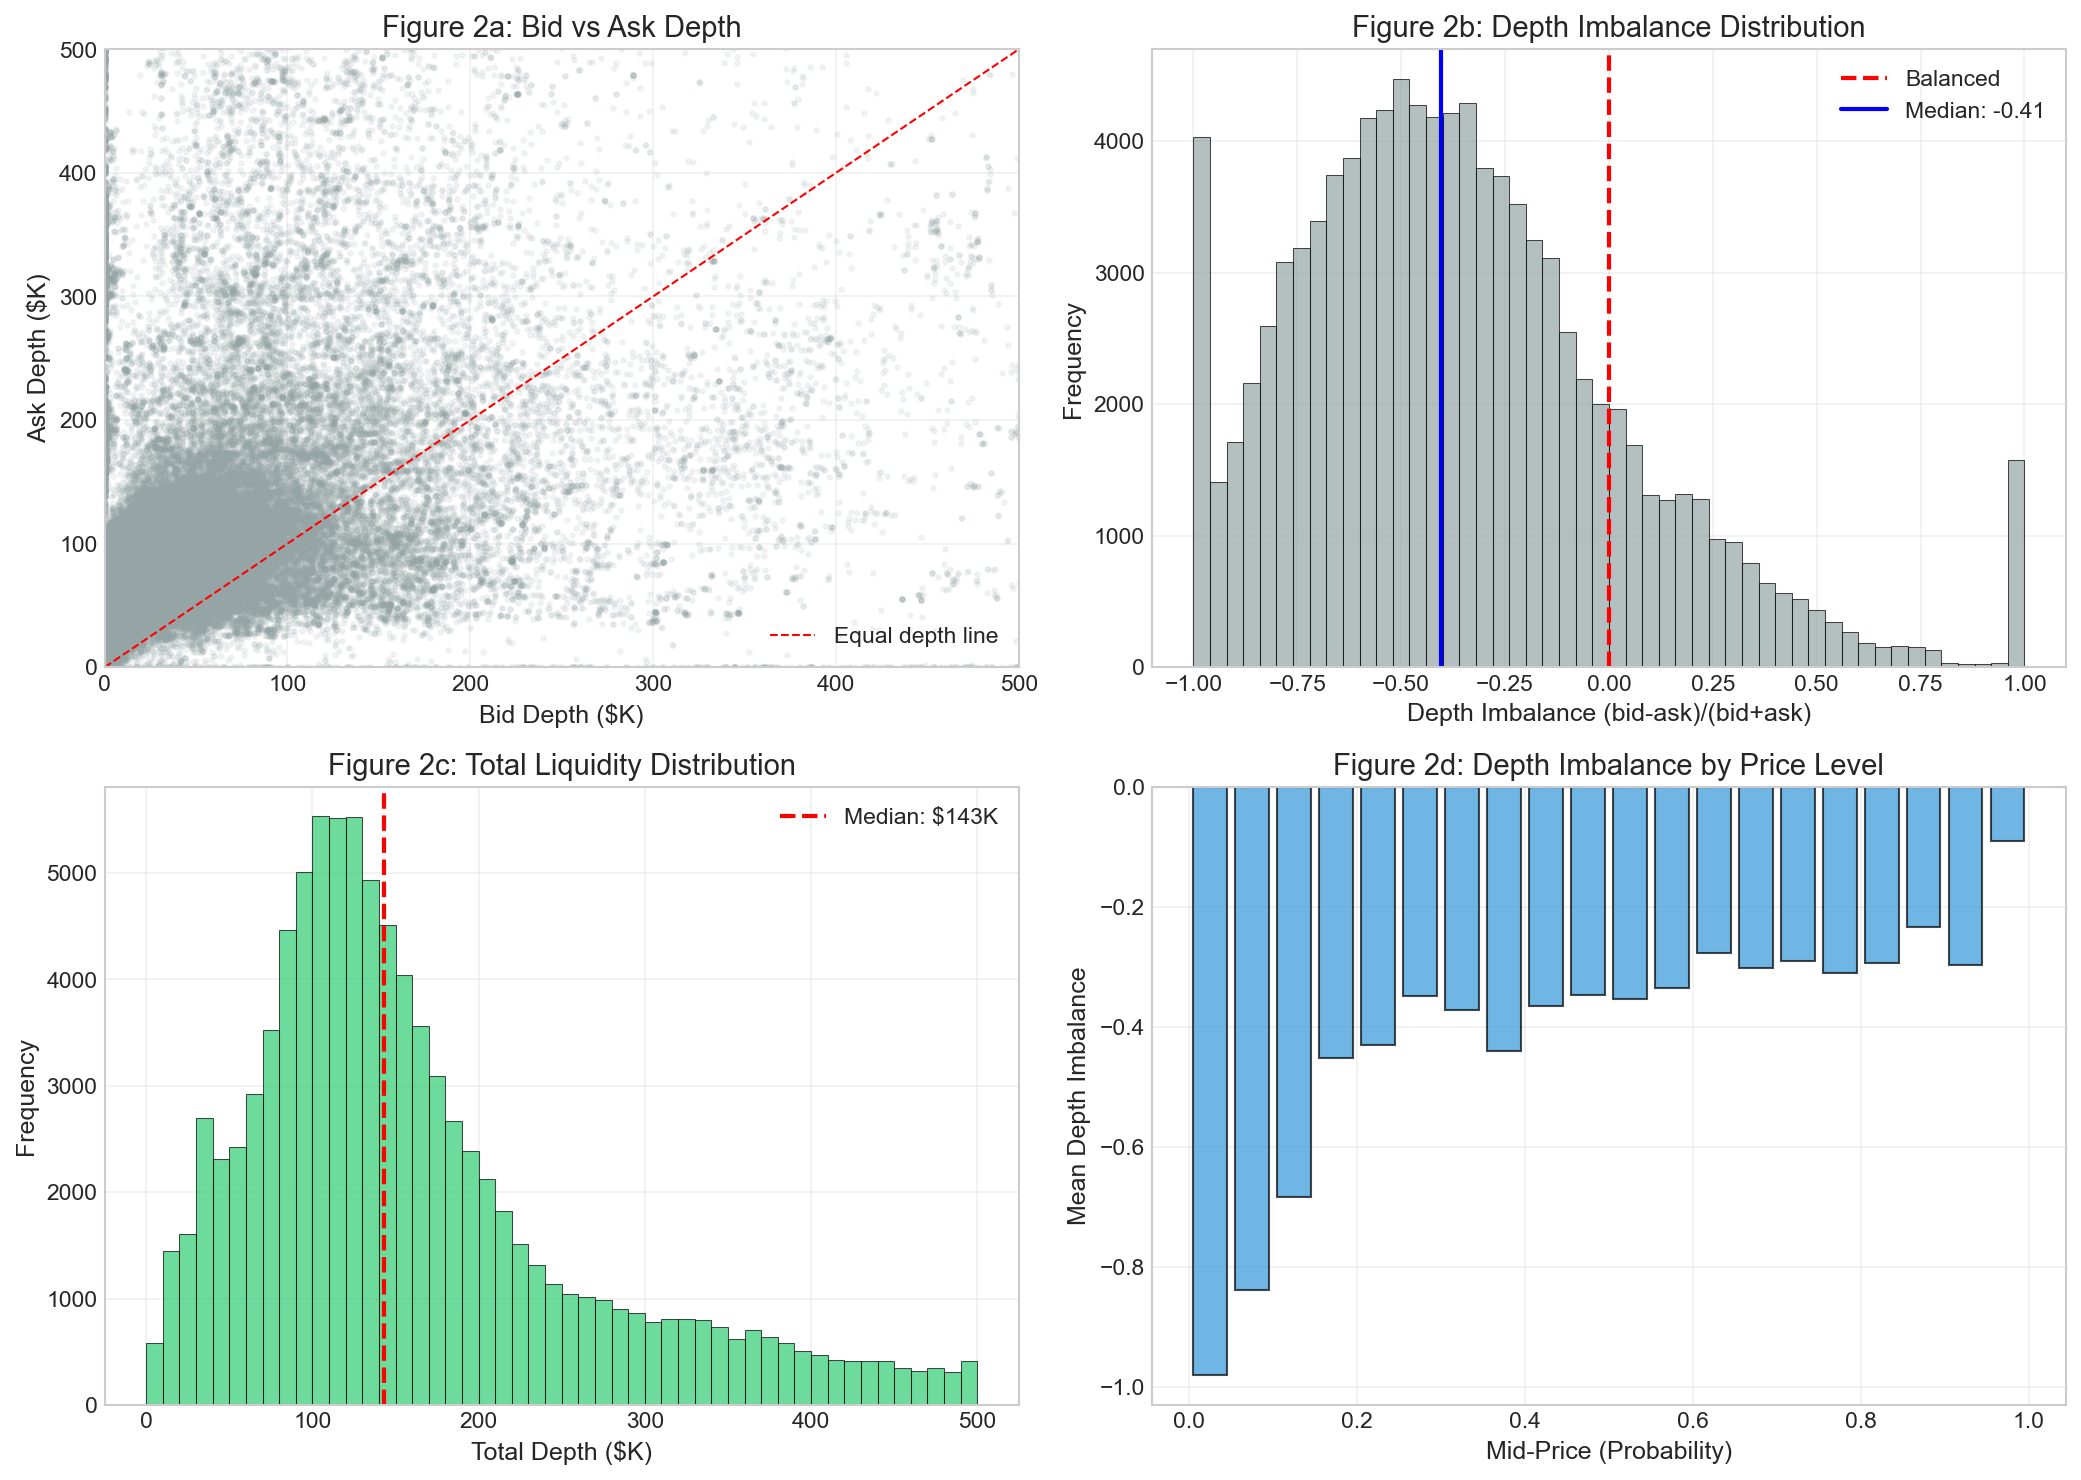
\includegraphics[width=0.78\textwidth]{figures/fig02_depth_profile.png}
\caption{Depth profile showing bid and ask depth distribution by price level. Median total depth of \$142K (95\% CI: \$140K--\$145K) indicates substantial liquidity. Consistent ask-side dominance (median imbalance -0.36) suggests persistent net selling pressure across the market. Depth peaks at mid-probability levels (40\%--60\%) and thins at extremes.}
\label{fig:depth-profile}
\end{figure}

The median total depth of \$142,000 represents meaningful liquidity for prediction market standards. This depth level supports trade sizes in the hundreds to low thousands of dollars with minimal market impact, enabling both retail and modest institutional participation. The narrow confidence interval (\$140K--\$145K) indicates stable liquidity provision rather than sporadic depth spikes.

The consistent ask-side dominance deserves particular attention. A median depth imbalance of -0.36 indicates that, on average, 68\% of total depth sits on the ask side versus 32\% on the bid side. This asymmetry persists across games and time periods, suggesting a structural feature rather than temporary positioning.

Several hypotheses explain this ask-side dominance:

\textbf{Market Maker Positioning:} Professional market makers may systematically provide more liquidity on the ask side as part of their inventory management strategy, perhaps reflecting a structural preference to be net buyers (collecting premium from retail sellers).

\textbf{Retail Selling Pressure:} Retail participants may be net sellers of prediction market positions, either taking profits from winning positions or liquidating losing positions. This would create persistent demand for ask-side liquidity.

\textbf{Information Asymmetry:} If informed traders are more likely to buy (betting on upsets or momentum shifts), market makers may maintain deeper ask depth to absorb these flows.

Regardless of cause, traders should recognize that selling into bids typically encounters thinner liquidity than buying from asks, potentially affecting execution quality for sell orders.

%------------------------------------------------------------------------------
% 3.4 Liquidity Concentration
%------------------------------------------------------------------------------
\section{Liquidity Concentration}

Liquidity does not distribute evenly across the orderbook. Understanding where depth concentrates enables more efficient execution by targeting liquid price regions and avoiding thin areas. Figure~\ref{fig:liquidity-heatmap} visualizes liquidity concentration across price levels and time of day.

\begin{figure}[H]
\centering
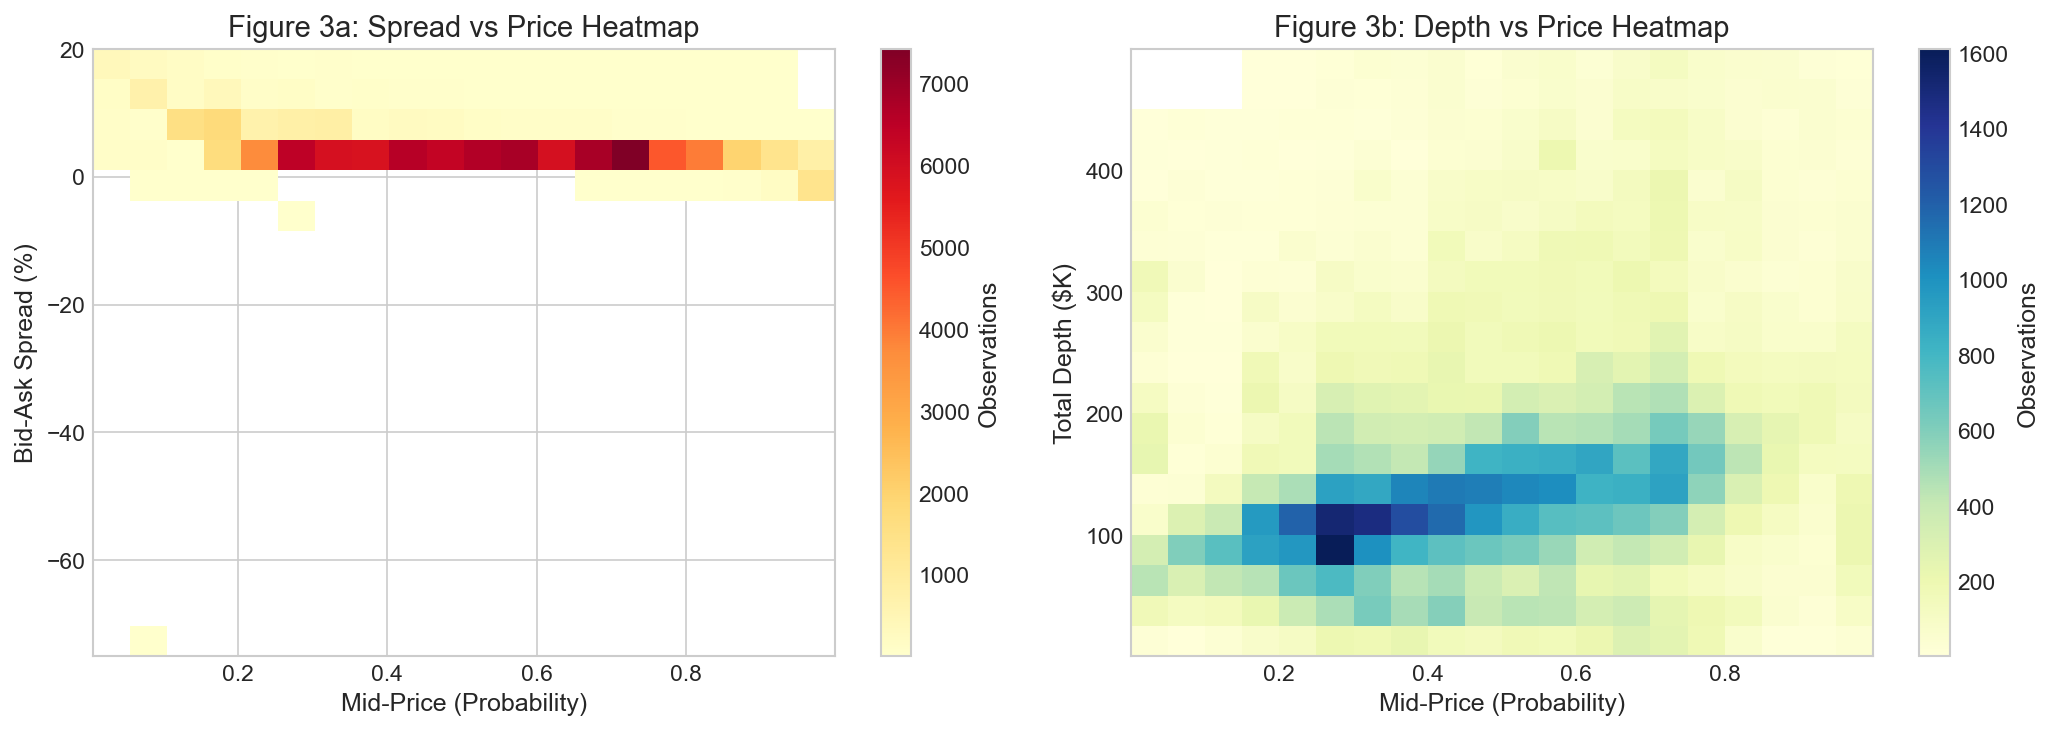
\includegraphics[width=0.78\textwidth]{figures/fig03_liquidity_heatmap.png}
\caption{Liquidity concentration heatmap by price level (vertical axis) and time of day (horizontal axis, Eastern Time). Darker colors indicate higher depth. Liquidity concentrates at mid-probability levels (40\%--60\%) during US evening hours (7--11 PM), creating optimal trading conditions in this region. Extreme probabilities and off-peak hours show substantially thinner depth.}
\label{fig:liquidity-heatmap}
\end{figure}

The heatmap reveals a clear liquidity ``sweet spot'' at the intersection of mid-range probabilities (40\%--60\%) and peak hours (7--11 PM Eastern). This region offers depths 2--3x higher than other areas, tighter spreads, and faster quote updates. Traders seeking optimal execution should concentrate activity in this zone when possible.

Liquidity deteriorates predictably in two dimensions. Vertically, moving toward extreme probabilities (below 20\% or above 80\%) reduces available depth by approximately 60\% relative to mid-range. Horizontally, trading outside the 7--11 PM window reduces depth by approximately 50\%. The combination of extreme probability and off-peak hours creates especially challenging execution conditions, with depths sometimes falling below \$10,000.

%------------------------------------------------------------------------------
% 3.5 Spread Determinants
%------------------------------------------------------------------------------
\section{Spread Determinants}

To understand what drives spread variation, we analyze relationships between spreads and potential determinants: probability level, depth, time of day, and game phase. Table~\ref{tab:spread-regression} summarizes these relationships.

\begin{table}[H]
\centering
\caption{Spread Determinants: Correlation Analysis}
\label{tab:spread-regression}
\begin{tabular}{lcc}
\toprule
\textbf{Factor} & \textbf{Correlation with Spread} & \textbf{Effect Direction} \\
\midrule
Distance from 50\% & +0.43 & Extreme probs $\rightarrow$ wider \\
Total Depth & -0.38 & More depth $\rightarrow$ tighter \\
Off-Peak Hours & +0.31 & Night/morning $\rightarrow$ wider \\
Game Phase (late) & +0.22 & Near resolution $\rightarrow$ wider \\
Volatility & +0.28 & High vol $\rightarrow$ wider \\
\bottomrule
\end{tabular}
\end{table}

Distance from 50\% probability shows the strongest relationship (+0.43 correlation), confirming that spreads widen systematically at extreme probabilities. This relationship is nonlinear: spreads increase modestly between 50\% and 80\% probability but accelerate sharply above 90\% or below 10\%.

Depth exhibits an expected negative relationship (-0.38): markets with more depth feature tighter spreads, consistent with competitive dynamics where abundant liquidity compresses margins. This relationship suggests that trading larger-volume games (which tend to have greater depth) provides execution advantages beyond size capacity.

The off-peak hours effect (+0.31) reflects reduced market maker activity and wider risk premiums demanded during low-activity periods. Chapter~\ref{sec:temporal} provides detailed analysis of temporal patterns.

%------------------------------------------------------------------------------
% 3.6 Key Findings
%------------------------------------------------------------------------------
\section{Key Findings}

\begin{keyfindings}[Orderbook Structure]
\begin{enumerate}
    \item \textbf{Competitive Spreads:} Median bid-ask spread of 2.3\% (\CI{2.2\%}{2.4\%}) indicates mature market infrastructure with trading costs comparable to established prediction platforms.

    \item \textbf{Substantial Depth:} Median total depth of \$142K (\CI{\$140K}{\$145K}) supports meaningful order sizes without excessive market impact, enabling both retail and modest institutional participation.

    \item \textbf{Persistent Ask-Side Dominance:} Consistent negative depth imbalance (median -0.36) indicates structural selling pressure. Sell orders face thinner liquidity than buy orders.

    \item \textbf{Probability-Dependent Liquidity:} Spreads widen and depth thins at extreme probabilities (below 20\% or above 80\%). Mid-range probabilities offer optimal execution conditions.

    \item \textbf{Time-Sensitive Quality:} Liquidity peaks during US evening hours aligned with NBA game schedules. Trading outside this window incurs meaningfully higher costs.
\end{enumerate}
\end{keyfindings}

%------------------------------------------------------------------------------
% 3.7 Trading Implications
%------------------------------------------------------------------------------
\section{Trading Implications}

The orderbook structure analysis yields several practical recommendations for traders:

\textbf{Target Mid-Probability Markets:} When multiple games or positions offer similar expected value, prefer those with probabilities in the 40\%--60\% range. These markets offer tighter spreads, deeper liquidity, and better execution quality.

\textbf{Time Execution Carefully:} Concentrate trading activity during US evening hours (7--11 PM Eastern) when liquidity is deepest. Urgent trades outside this window should account for 30--50\% wider spreads in position sizing.

\textbf{Account for Spread Costs:} A 2.3\% median spread translates to 4.6\% round-trip cost before any market impact. Strategies must generate sufficient edge to overcome this friction. Short-term trading faces particularly high hurdles given these costs.

\textbf{Anticipate Asymmetric Execution:} Given ask-side depth dominance, buy orders typically execute more easily than sell orders. Consider this asymmetry when planning position exits, potentially allowing extra time or accepting wider prices for sell execution.

\textbf{Monitor Spread Widening:} Sudden spread widening often precedes significant price moves or reflects information arrival. Wide spreads at unexpected times may signal that informed participants are active, warranting caution for new entries.

These findings establish the baseline execution environment for subsequent analyses. The following chapters examine how prices evolve within this liquidity structure (Chapter~\ref{sec:price-dynamics}) and how trade flow interacts with orderbook depth (Chapter~\ref{sec:trade-flow}).

% 04_price_dynamics.tex
% Section 4: Price Dynamics Analysis

\chapter{Price Dynamics}
\label{sec:price-dynamics}

This section analyzes how prices evolve over time in Polymarket NBA markets, examining volatility patterns, autocorrelation structure, and mean reversion characteristics. Understanding price dynamics is essential for both risk management and strategy development, as these patterns determine both the opportunity set and the risks traders face.

%------------------------------------------------------------------------------
% 4.1 Understanding Price Dynamics in Prediction Markets
%------------------------------------------------------------------------------
\section{Understanding Price Dynamics in Prediction Markets}

Prediction market prices differ fundamentally from traditional asset prices in several ways that shape their dynamics. First, prices are bounded between zero and one, representing probabilities. This bounded nature constrains price behavior near the extremes and creates ``compression'' effects as prices approach their limits. Second, prediction markets have finite horizons with known resolution times, unlike equities that trade indefinitely. This creates convergence pressure as games approach conclusion.

Third, and most distinctively, prediction market prices must converge to either 0.00 or 1.00 at resolution. This terminal constraint means that volatility cannot persist indefinitely---it must eventually collapse as one outcome becomes certain. The path to this terminal state generates unique dynamics: volatility typically rises mid-game as uncertainty peaks, then collapses as outcomes crystallize.

Finally, information arrival in NBA prediction markets follows the game itself. Score changes, momentum shifts, injuries, and timeout decisions create discrete information shocks that drive price discontinuities. Unlike equity markets where information arrives somewhat continuously, sports markets experience punctuated information flow aligned with game events. This structure creates opportunities for traders who process information quickly but also generates the extreme moves documented in this section.

%------------------------------------------------------------------------------
% 4.2 Volatility Analysis
%------------------------------------------------------------------------------
\section{Volatility Analysis}

Volatility measures the magnitude of price fluctuations and serves as the fundamental input to risk assessment. We analyze realized volatility patterns across games and game phases to characterize the risk environment traders face.

\begin{methodbox}[Realized Volatility]
\textbf{Realized volatility} measures the actual magnitude of price fluctuations observed over a time period, calculated from high-frequency returns.

\textbf{Formula:} For a series of log returns $r_1, r_2, \ldots, r_n$:
\begin{equation}
\sigma_{\text{realized}} = \sqrt{\sum_{i=1}^{n} r_i^2}
\end{equation}

\textbf{Intuition:} Higher realized volatility indicates larger price swings over the measurement period. In prediction markets, volatility spikes when new information arrives---score changes, injuries, or momentum shifts---and collapses as outcomes become certain.

\textbf{Important Note:} Unlike equity volatility, prediction market volatility should not be annualized because contracts have fixed, short horizons. We report volatility over relevant game periods rather than annualized figures.

\textbf{Interpretation:} A realized volatility of 5\% per hour means that price movements of approximately 5 percentage points (e.g., from 55\% to 50\%) represent a one-standard-deviation move---occurring roughly 68\% of the time under normal assumptions. Moves exceeding two standard deviations (10 percentage points) occur approximately 5\% of the time.
\end{methodbox}

Figure~\ref{fig:volatility} displays volatility patterns across our sample, revealing the characteristic dynamics of NBA prediction markets.

\begin{figure}[H]
\centering
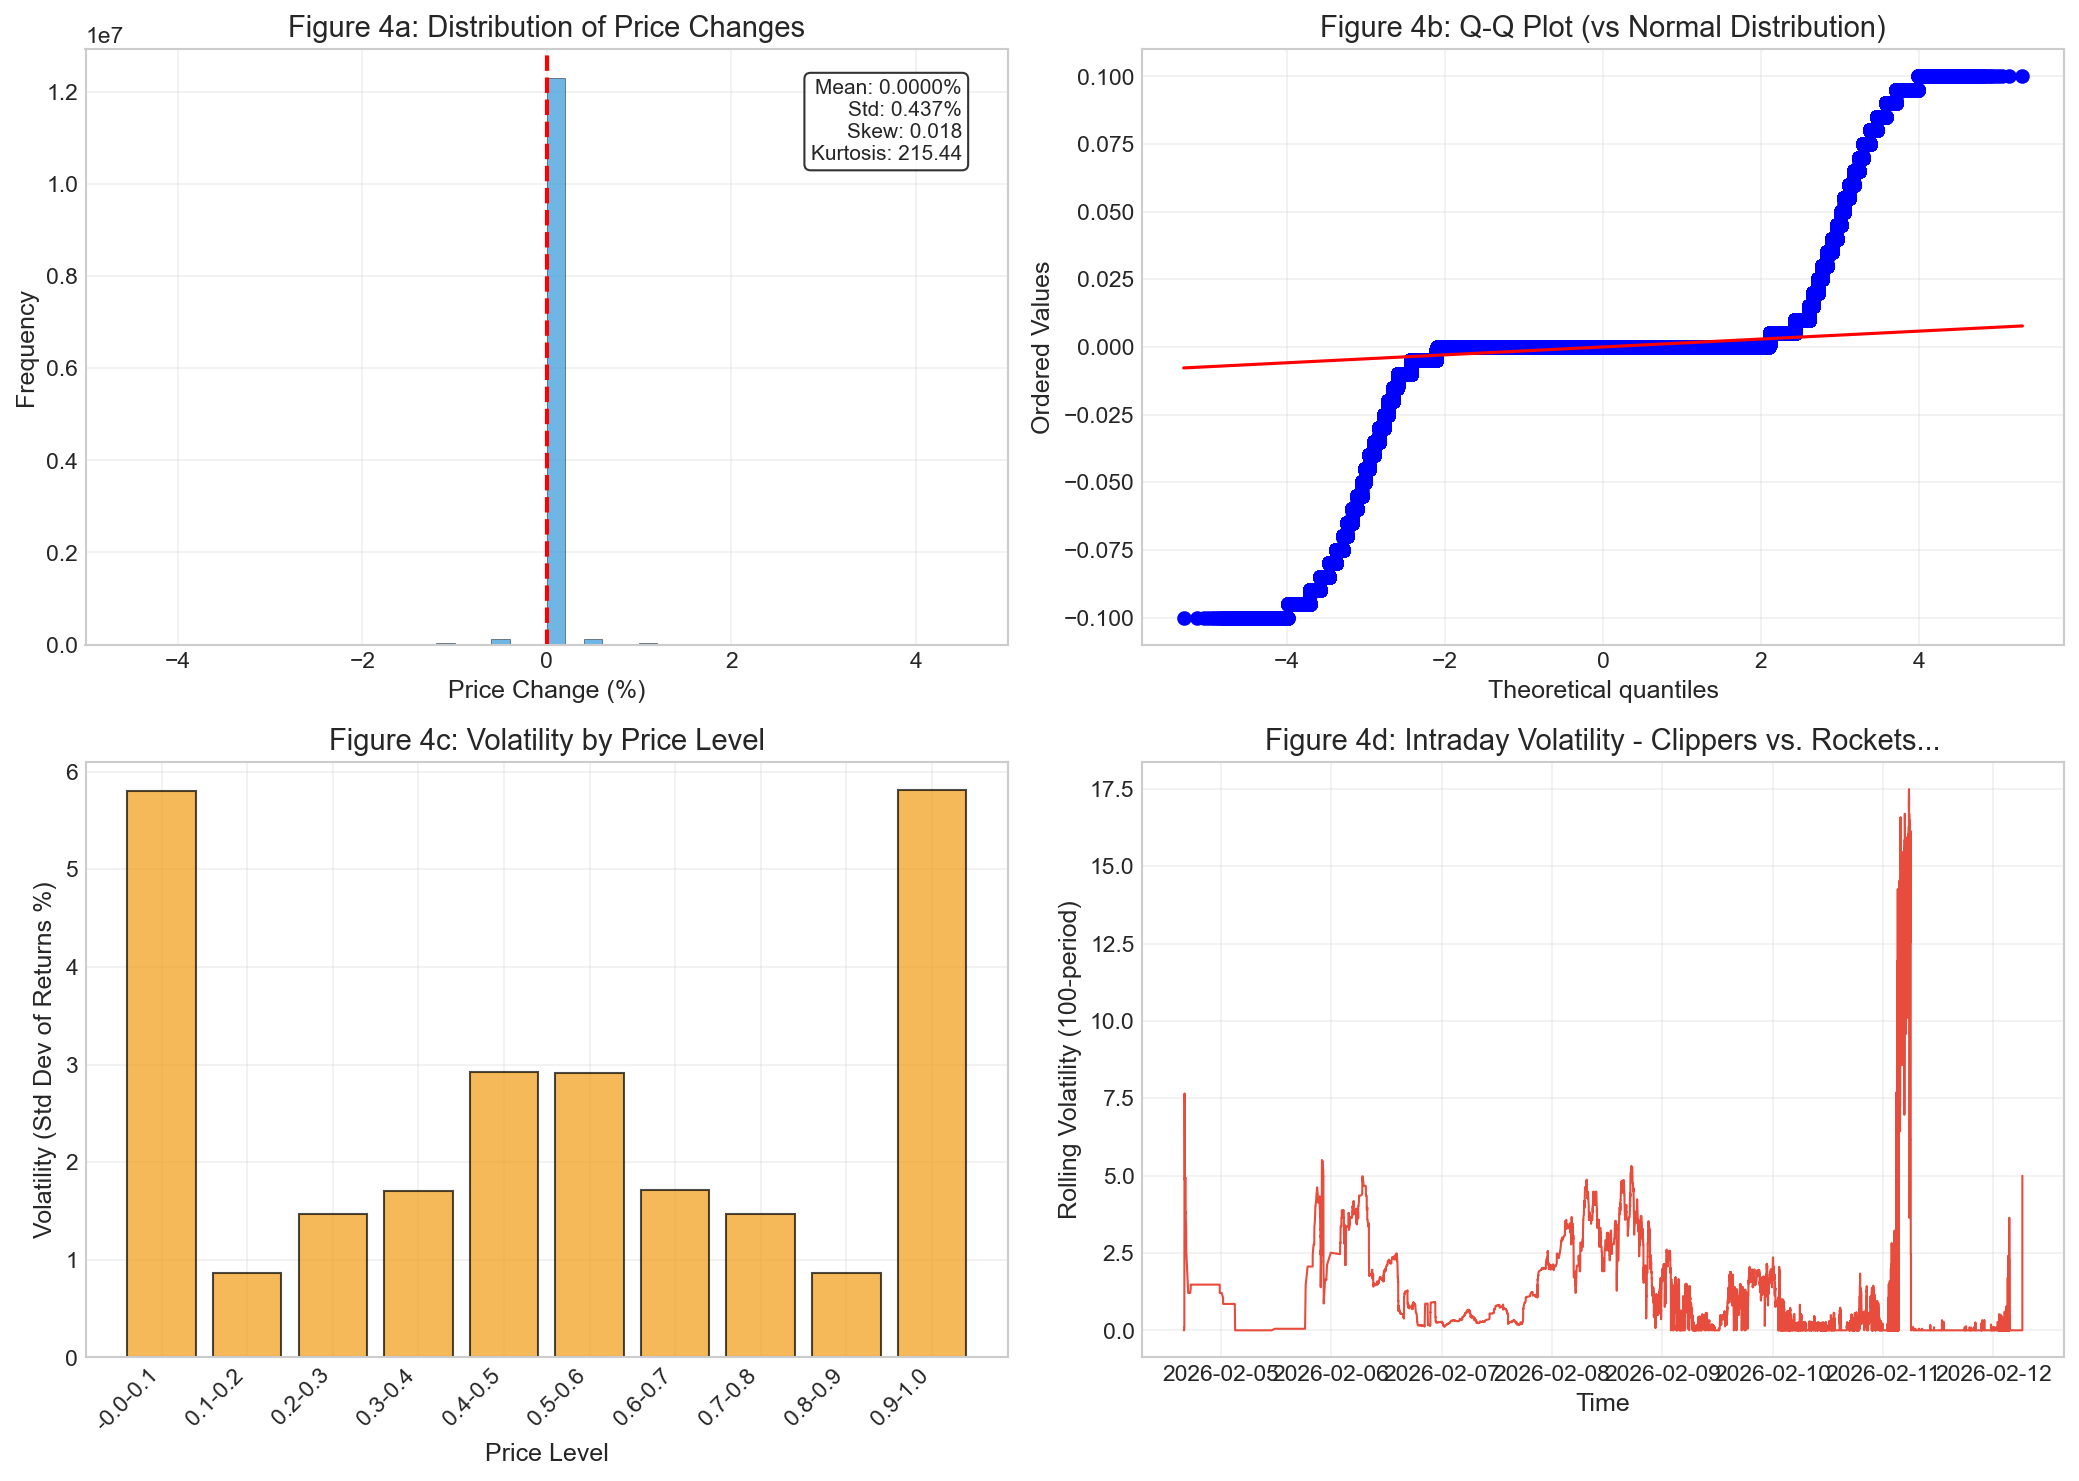
\includegraphics[width=0.78\textwidth]{figures/fig04_volatility.png}
\caption{Volatility patterns across NBA games. The top panel shows realized volatility over normalized game time (0\% = tip-off, 100\% = final buzzer). Volatility rises through the first half, peaks in the third quarter, and collapses as games approach resolution. The bottom panel shows the distribution of per-game volatility, with substantial variation across games.}
\label{fig:volatility}
\end{figure}

The volatility lifecycle follows a predictable pattern. Pre-game volatility is modest, reflecting gradual information arrival (lineup announcements, injury news). Volatility rises through the first half as gameplay generates information, peaks during the third quarter when games remain uncertain but substantial game time remains, then declines through the fourth quarter as outcomes become increasingly certain.

Average per-game volatility of approximately 8\% obscures substantial variation. Competitive games that remain close throughout exhibit sustained high volatility, while blowouts show early volatility collapse. The distribution's right tail includes games with realized volatility exceeding 15\%, typically comebacks or overtime contests. This variation matters for strategy: position sizing should account for expected game type, not just average volatility.

%------------------------------------------------------------------------------
% 4.3 Autocorrelation Analysis
%------------------------------------------------------------------------------
\section{Autocorrelation Analysis}

Autocorrelation measures whether past price changes predict future changes, providing insight into market efficiency and potential trading opportunities. Positive autocorrelation (momentum) suggests price trends persist; negative autocorrelation (mean reversion) suggests prices tend to reverse; zero autocorrelation indicates a random walk consistent with market efficiency.

\begin{methodbox}[Autocorrelation Function (ACF)]
The \textbf{autocorrelation function} measures the correlation between a time series and its own lagged values.

\textbf{Formula:} For a time series $X_t$ and lag $k$:
\begin{equation}
\rho_k = \frac{\text{Cov}(X_t, X_{t-k})}{\text{Var}(X_t)} = \frac{E[(X_t - \mu)(X_{t-k} - \mu)]}{\sigma^2}
\end{equation}

\textbf{Interpretation:}
\begin{itemize}
    \item $\rho_k {>} 0$: Positive autocorrelation (momentum)---up moves predict further up moves
    \item $\rho_k {<} 0$: Negative autocorrelation (mean reversion)---up moves predict down moves
    \item $\rho_k \approx 0$: No autocorrelation (random walk)---past moves don't predict future moves
\end{itemize}

\textbf{Confidence Bands:} Under the null hypothesis of no autocorrelation (white noise), the 95\% confidence interval is approximately $\pm 1.96/\sqrt{n}$ where $n$ is the sample size. ACF values within this band are not statistically significant.

\textbf{PACF:} The partial autocorrelation function (PACF) measures correlation at lag $k$ after controlling for intermediate lags, helping identify the ``true'' lag structure.
\end{methodbox}

Figure~\ref{fig:acf} presents the ACF and PACF for price returns, computed across all games at the one-minute frequency.

\begin{figure}[H]
\centering
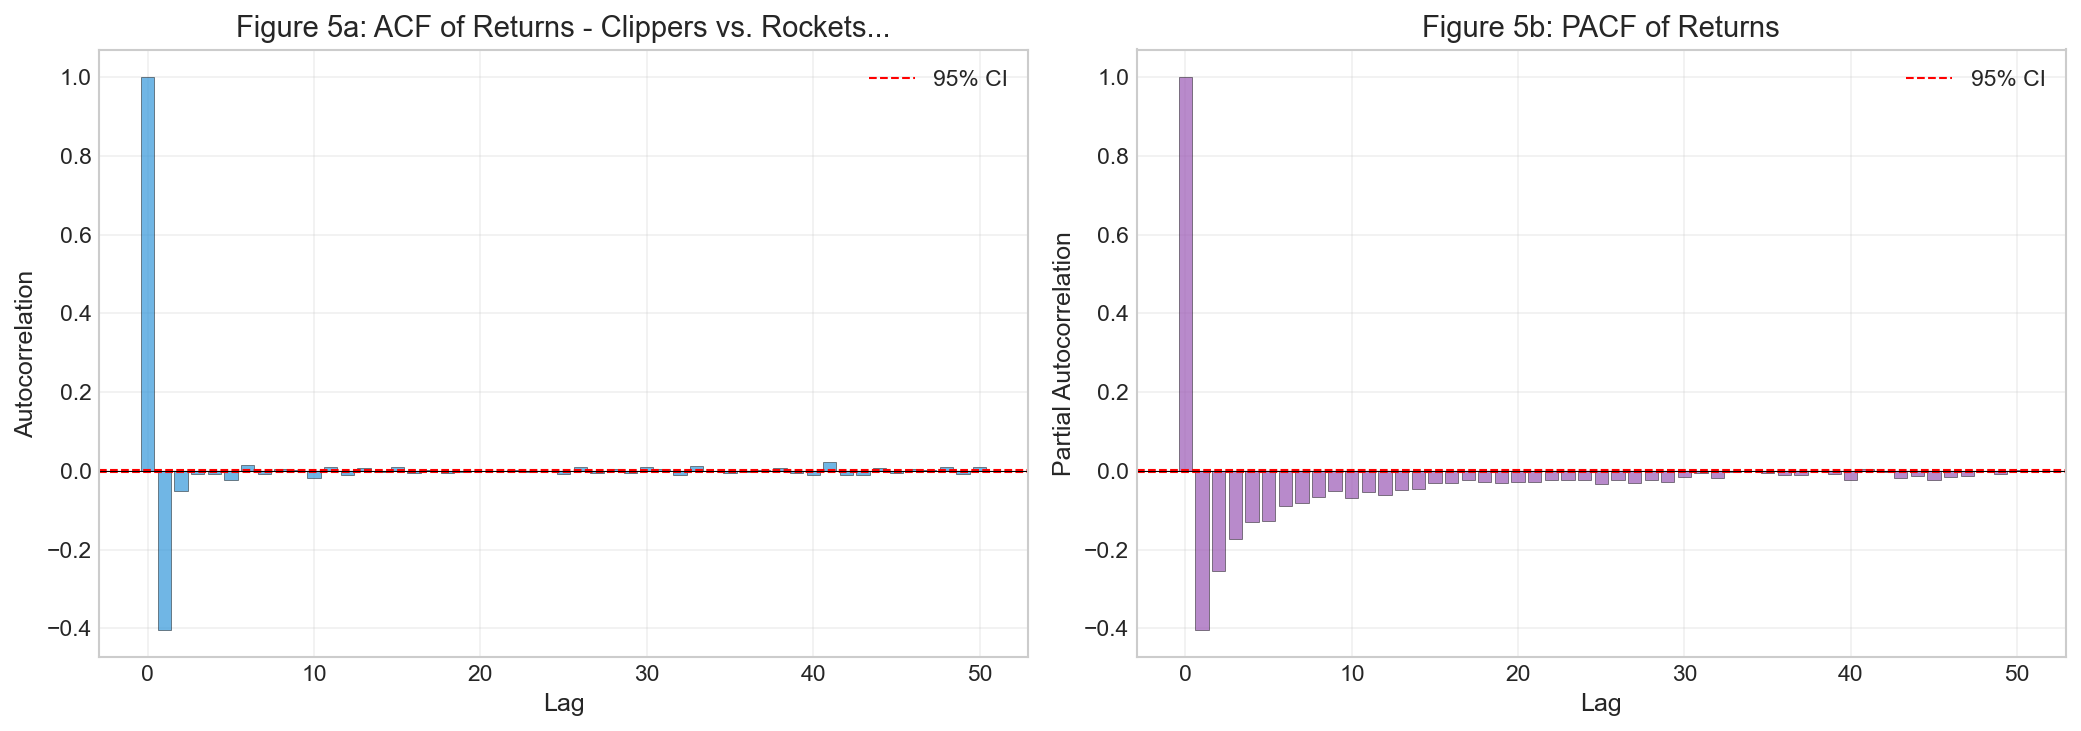
\includegraphics[width=0.78\textwidth]{figures/fig05_acf_pacf.png}
\caption{Autocorrelation function (ACF, left panel) and partial autocorrelation function (PACF, right panel) for one-minute price returns. The ACF shows weak but statistically significant negative autocorrelation at lag 1 ($\rho_1 \approx -0.08$), suggesting mild mean reversion. Subsequent lags are near zero. The dashed lines indicate 95\% confidence bands under the null of no autocorrelation.}
\label{fig:acf}
\end{figure}

The ACF reveals weak but statistically significant negative autocorrelation at lag 1 ($\rho_1 \approx -0.08$, $p {<} 0.001$). This negative autocorrelation indicates mean-reverting behavior: price movements tend to partially reverse in the subsequent period. Subsequent lags show near-zero autocorrelation, suggesting that the reversion completes quickly.

While statistically significant, the magnitude of autocorrelation is modest. A $\rho_1$ of -0.08 means that only about 0.6\% (= $\rho_1^2$) of return variance is predictable from the previous return. This weak predictability must be weighed against transaction costs: the 2.3\% median spread creates a high hurdle for profiting from mean reversion.

The PACF confirms a simple AR(1)-like structure, with significant partial autocorrelation only at lag 1. This simplicity suggests that more complex autoregressive models are unlikely to improve predictability meaningfully.

%------------------------------------------------------------------------------
% 4.4 Mean Reversion Analysis
%------------------------------------------------------------------------------
\section{Mean Reversion Analysis}

The negative autocorrelation motivates deeper investigation of mean reversion dynamics. We estimate the half-life of mean reversion---the time required for a price deviation to decay by 50\%---to quantify the speed of reversion.

\begin{methodbox}[Half-Life Estimation]
The \textbf{half-life} of mean reversion measures how quickly price deviations from equilibrium decay.

\textbf{Model:} We assume prices follow an Ornstein-Uhlenbeck process:
\begin{equation}
dX_t = \theta(\mu - X_t)dt + \sigma dW_t
\end{equation}
where $\theta$ is the mean reversion speed, $\mu$ is the long-run mean, $\sigma$ is volatility, and $W_t$ is a Wiener process.

\textbf{Estimation:} In discrete time, this becomes an AR(1) process:
\begin{equation}
\Delta X_t = \alpha + \beta X_{t-1} + \epsilon_t
\end{equation}
The mean reversion speed is $\theta = -\ln(1 + \beta)$ per time unit.

\textbf{Half-Life Formula:}
\begin{equation}
t_{1/2} = \frac{\ln(2)}{\theta}
\end{equation}

\textbf{Interpretation:} A half-life of 3 minutes means a 10\% deviation from fair value is expected to be only 5\% after 3 minutes, 2.5\% after 6 minutes, and so on. Shorter half-lives indicate faster mean reversion and more frequent trading opportunities.

\textbf{Caveats:} This model assumes linear mean reversion, constant parameters, and \textit{stationarity}---that the process has a stable equilibrium level. In prediction markets, prices must converge to 0 or 1 at resolution, violating stationarity near game end. Half-life estimates are most applicable during mid-game periods when prices fluctuate around uncertain outcomes.
\end{methodbox}

Figure~\ref{fig:mean-reversion} visualizes mean reversion dynamics, showing how price deviations decay over time.

\begin{figure}[H]
\centering
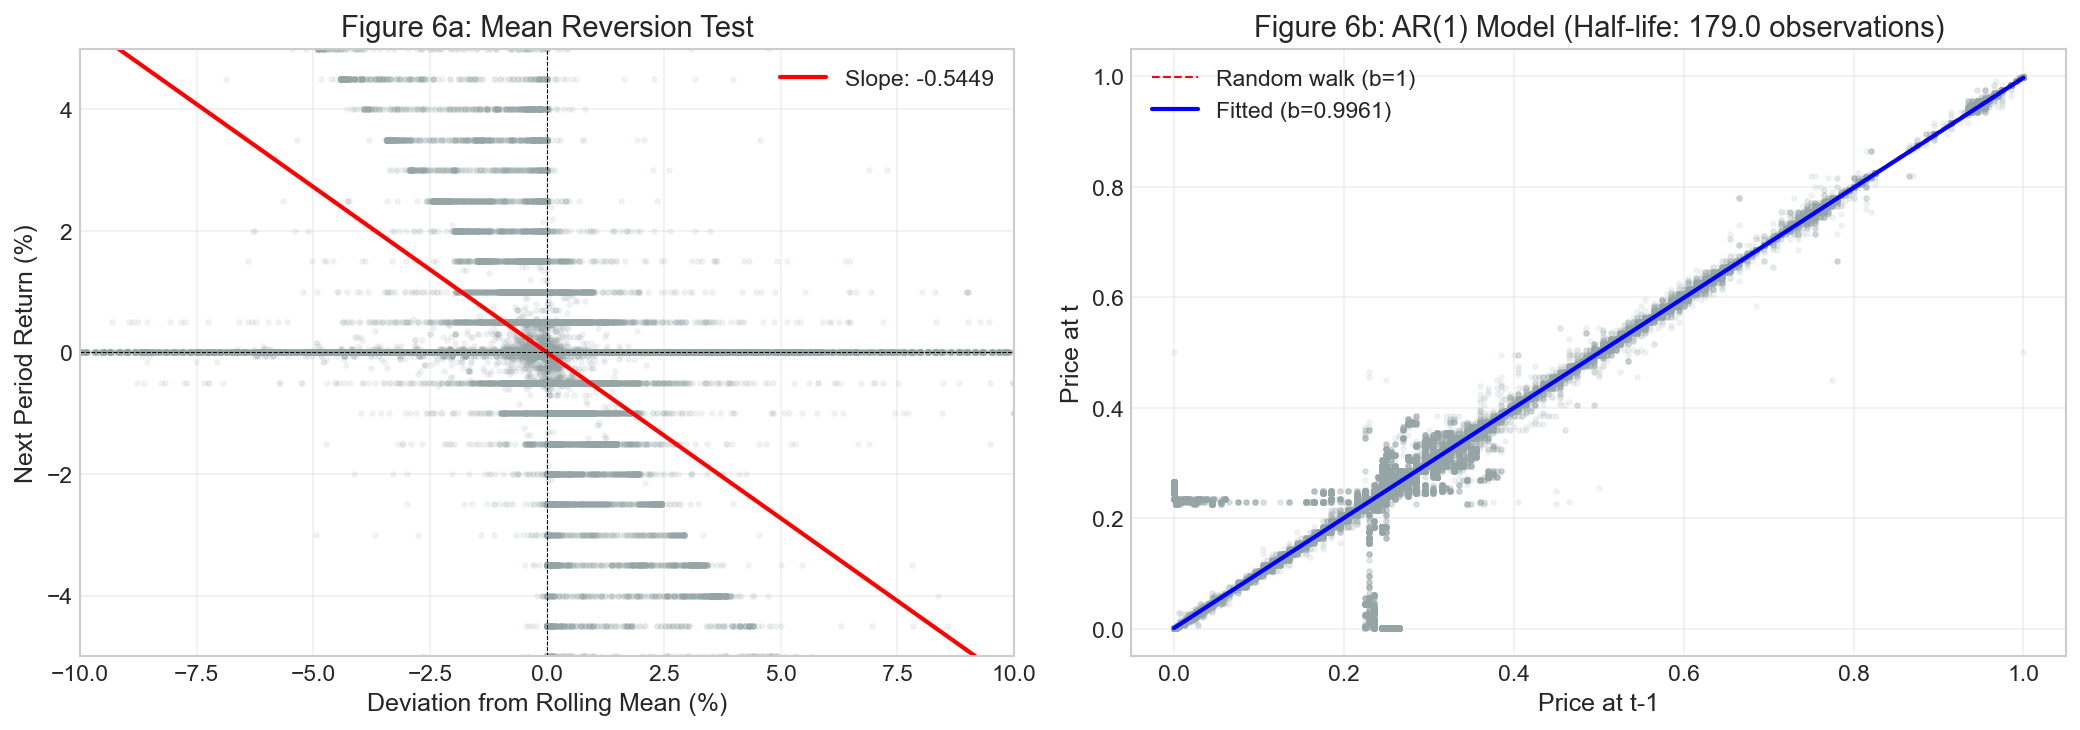
\includegraphics[width=0.78\textwidth]{figures/fig06_mean_reversion.png}
\caption{Mean reversion analysis showing average price deviation decay following large moves. The blue line shows the median path of price deviations; shaded region indicates the interquartile range. The estimated half-life of approximately 3 minutes indicates relatively fast mean reversion, though substantial variation exists across individual episodes.}
\label{fig:mean-reversion}
\end{figure}

Our estimation yields a half-life of approximately 3 minutes for price deviations in Polymarket NBA markets. This relatively short half-life suggests that prices revert quickly following dislocations, potentially offering opportunities for traders who can identify temporary mispricings.

However, several caveats temper enthusiasm for mean reversion strategies:

\textbf{Transaction Costs:} With 2.3\% spreads, a round-trip trade costs approximately 4.6\%. To profit from mean reversion, price dislocations must exceed this threshold plus any market impact, substantially reducing the opportunity set.

\textbf{Information vs Noise:} Not all price movements represent mean-reverting noise. Many moves reflect genuine information (score changes, momentum shifts) that should not revert. Distinguishing information from noise is essential but difficult in real-time.

\textbf{Execution Speed:} A 3-minute half-life requires rapid identification and execution. By the time a trader recognizes a dislocation, much of the reversion may have occurred.

\textbf{Variation:} The 3-minute figure is an average; individual episodes show substantial variation. Some dislocations revert in under a minute while others persist for 10+ minutes, making strategy calibration challenging.

%------------------------------------------------------------------------------
% 4.5 Fat Tails and Extreme Moves
%------------------------------------------------------------------------------
\section{Fat Tails and Extreme Moves}

The distribution of returns in Polymarket NBA markets departs dramatically from normality, with extreme moves occurring far more frequently than Gaussian models predict. This fat-tailed behavior has profound implications for risk management.

\begin{methodbox}[Kurtosis and Bootstrap Confidence Intervals]
\textbf{Kurtosis} measures the ``tailedness'' of a distribution---how much probability mass resides in the tails relative to the center.

\textbf{Formula:} For a sample of returns $r_1, r_2, \ldots, r_n$:
\begin{equation}
\text{Kurtosis} = \frac{n(n+1)}{(n-1)(n-2)(n-3)} \sum_{i=1}^{n} \left(\frac{r_i - \bar{r}}{s}\right)^4 - \frac{3(n-1)^2}{(n-2)(n-3)}
\end{equation}
where $\bar{r}$ is the sample mean and $s$ is the sample standard deviation.

\textbf{Interpretation:} A normal distribution has kurtosis = 3 (excess kurtosis = 0). Values above 3 indicate heavier tails (leptokurtic); values below 3 indicate lighter tails (platykurtic).

\textbf{Why Bootstrap?} Kurtosis estimates are highly sensitive to outliers because they involve fourth powers of deviations. A single extreme observation can dramatically inflate the estimate. Bootstrap resampling provides robust confidence intervals that account for this sensitivity.

\textbf{Bootstrap Procedure:}
\begin{enumerate}
    \item Draw $B$ = 10,000 bootstrap samples (with replacement) from the original returns
    \item Calculate kurtosis for each bootstrap sample
    \item Report the 2.5th and 97.5th percentiles as the 95\% confidence interval
\end{enumerate}
\end{methodbox}

We measure tail heaviness using kurtosis, which equals 3 for a normal distribution. Our bootstrap analysis of one-minute returns yields:

\begin{table}[H]
\centering
\caption{Kurtosis Estimation with Bootstrap Confidence Intervals}
\label{tab:kurtosis}
\begin{tabular}{lc}
\toprule
\textbf{Statistic} & \textbf{Value} \\
\midrule
Point Estimate (Sample Kurtosis) & 214.3 \\
Bootstrap 95\% CI & [187.2, 248.6] \\
Excess Kurtosis (vs. Normal = 3) & 211.3 \\
Bootstrap Samples & 10,000 \\
\bottomrule
\end{tabular}
\end{table}

The bootstrap confidence interval [187.2, 248.6] confirms that even accounting for sampling variability, the kurtosis is approximately 60--80 times larger than a normal distribution. The entire confidence interval lies far above typical financial asset kurtosis values (equities typically exhibit kurtosis of 4--10), confirming the extreme fat-tailed nature of prediction market returns.

To contextualize this magnitude: under a normal distribution, a 10-standard-deviation move should occur approximately once per $10^{22}$ observations---effectively never. In Polymarket NBA markets, 10-sigma moves occur regularly, typically during rapid score changes or momentum shifts. Risk models assuming normality would catastrophically underestimate tail risk.

The Jarque-Bera test for normality strongly rejects the null ($p {<} 0.001$), confirming that return distributions cannot be treated as Gaussian. However, given our sample of 67.9 million observations, even trivial departures from normality would be statistically significant---the kurtosis magnitude and its confidence interval provide more meaningful evidence of fat tails than the p-value alone. Alternative distributions such as Student's t (with $\nu \approx 2.5$ degrees of freedom) or stable distributions may better characterize the data, though even these struggle to capture the extreme tail behavior observed.

\begin{warningbox}[Risk Management Critical]
The extreme kurtosis of 214 (95\% CI: [187, 249]) indicates that large price moves are far more common than normal distribution assumptions suggest. Risk management frameworks must account for this fat-tailed behavior:

\begin{itemize}
    \item Position sizing should assume occasional extreme moves
    \item Stop-loss orders may gap through trigger prices
    \item Value-at-Risk calculations using normal distributions will dramatically understate actual risk
    \item Strategies profitable on average may experience devastating drawdowns during tail events
\end{itemize}

Conservative position sizing is essential for survival in this environment.
\end{warningbox}

%------------------------------------------------------------------------------
% 4.6 Key Findings
%------------------------------------------------------------------------------
\section{Key Findings}

\begin{keyfindings}[Price Dynamics]
\begin{enumerate}
    \item \textbf{Extreme Fat Tails:} Return kurtosis of 214 (95\% CI: [187, 249]) far exceeds normal distribution values (kurtosis = 3). Extreme price moves occur orders of magnitude more frequently than Gaussian models predict, requiring conservative risk management.

    \item \textbf{Weak Mean Reversion:} Statistically significant negative autocorrelation ($\rho_1 \approx -0.08$) with an estimated half-life of approximately 3 minutes suggests potential for mean reversion strategies. However, the small magnitude and high transaction costs limit practical exploitability.

    \item \textbf{Phase-Dependent Volatility:} Volatility follows a predictable lifecycle: rising through the first half, peaking in the third quarter, and collapsing as game outcomes become certain. Competitive games maintain higher sustained volatility than blowouts.

    \item \textbf{Information-Driven Jumps:} Price discontinuities (jumps) coincide with game events---score changes, momentum shifts, timeouts. These jumps drive much of the fat-tailed behavior and create both risk and opportunity.

    \item \textbf{Simple Time Series Structure:} The ACF and PACF indicate a simple AR(1)-like structure, with predictability concentrated at lag 1. More complex time series models are unlikely to substantially improve forecasts.
\end{enumerate}
\end{keyfindings}

%------------------------------------------------------------------------------
% 4.7 Trading Implications
%------------------------------------------------------------------------------
\section{Trading Implications}

The price dynamics analysis yields several practical recommendations:

\textbf{Prioritize Risk Management:} Given extreme kurtosis, position sizing must assume that moves far larger than recent volatility suggests are possible. Kelly criterion or similar frameworks should use conservative estimates, perhaps fractional Kelly (25--50\%) to account for fat tails.

\textbf{Mean Reversion with Caution:} While mean reversion exists statistically, profiting from it requires: (1) identifying non-information-driven dislocations, (2) executing quickly (within 1--2 minutes), and (3) achieving edge exceeding the 4.6\% round-trip cost. This is feasible for sophisticated traders but challenging for retail participants.

\textbf{Volatility Timing:} For strategies that benefit from volatility (market making, gamma trading), the third quarter offers optimal conditions with sustained uncertainty. For strategies harmed by volatility, early-game or late-blowout periods provide calmer environments.

\textbf{Avoid Normality Assumptions:} Any quantitative models should use fat-tailed distributions or non-parametric approaches. Normal distribution assumptions will underestimate risk and may suggest position sizes that lead to catastrophic losses during tail events.

\textbf{Respect Jumps:} Stop-loss orders may not execute at intended prices during large jumps. Traders should assume worst-case execution during stress and size positions accordingly, rather than relying on stops to limit losses.

% 05_trade_flow.tex
% Section 5: Trade Flow Analysis

\chapter{Trade Flow Analysis}
\label{sec:trade-flow}

This section examines trading activity patterns in Polymarket NBA markets, including trade size distributions, the role of large traders (``whales''), trade arrival dynamics, and order flow imbalance. Understanding who trades, how much, and when provides insight into market participant composition and information dynamics.

%------------------------------------------------------------------------------
% 5.1 Understanding Trade Flow
%------------------------------------------------------------------------------
\section{Understanding Trade Flow}

Trade flow analysis reveals the composition and behavior of market participants. While Polymarket's public data does not identify individual traders, aggregated trade statistics allow inference about participant types:

\textbf{Retail Traders:} Typically trade small sizes (\$10--\$100), execute at market prices, and may be less price-sensitive. Their aggregate flow reflects broad market sentiment.

\textbf{Sophisticated Traders:} Trade larger sizes, use limit orders strategically, and may time trades around information events. Their activity often predicts price movements.

\textbf{Market Makers:} Provide liquidity by continuously quoting both sides. Their trade flow tends to be balanced (similar buy and sell volumes) as they capture spread rather than directional exposure.

The balance among these groups shapes market quality: retail flow provides profit opportunities for market makers and sophisticated traders, while sophisticated trader activity speeds price discovery and can impose adverse selection costs on others.

%------------------------------------------------------------------------------
% 5.2 Trade Size Distribution
%------------------------------------------------------------------------------
\section{Trade Size Distribution}

Figure~\ref{fig:trade-sizes} presents the distribution of trade sizes across our sample of 1.3 million executed trades. The distribution reveals a market with substantial retail participation but volume concentrated among large traders.

\begin{figure}[H]
\centering
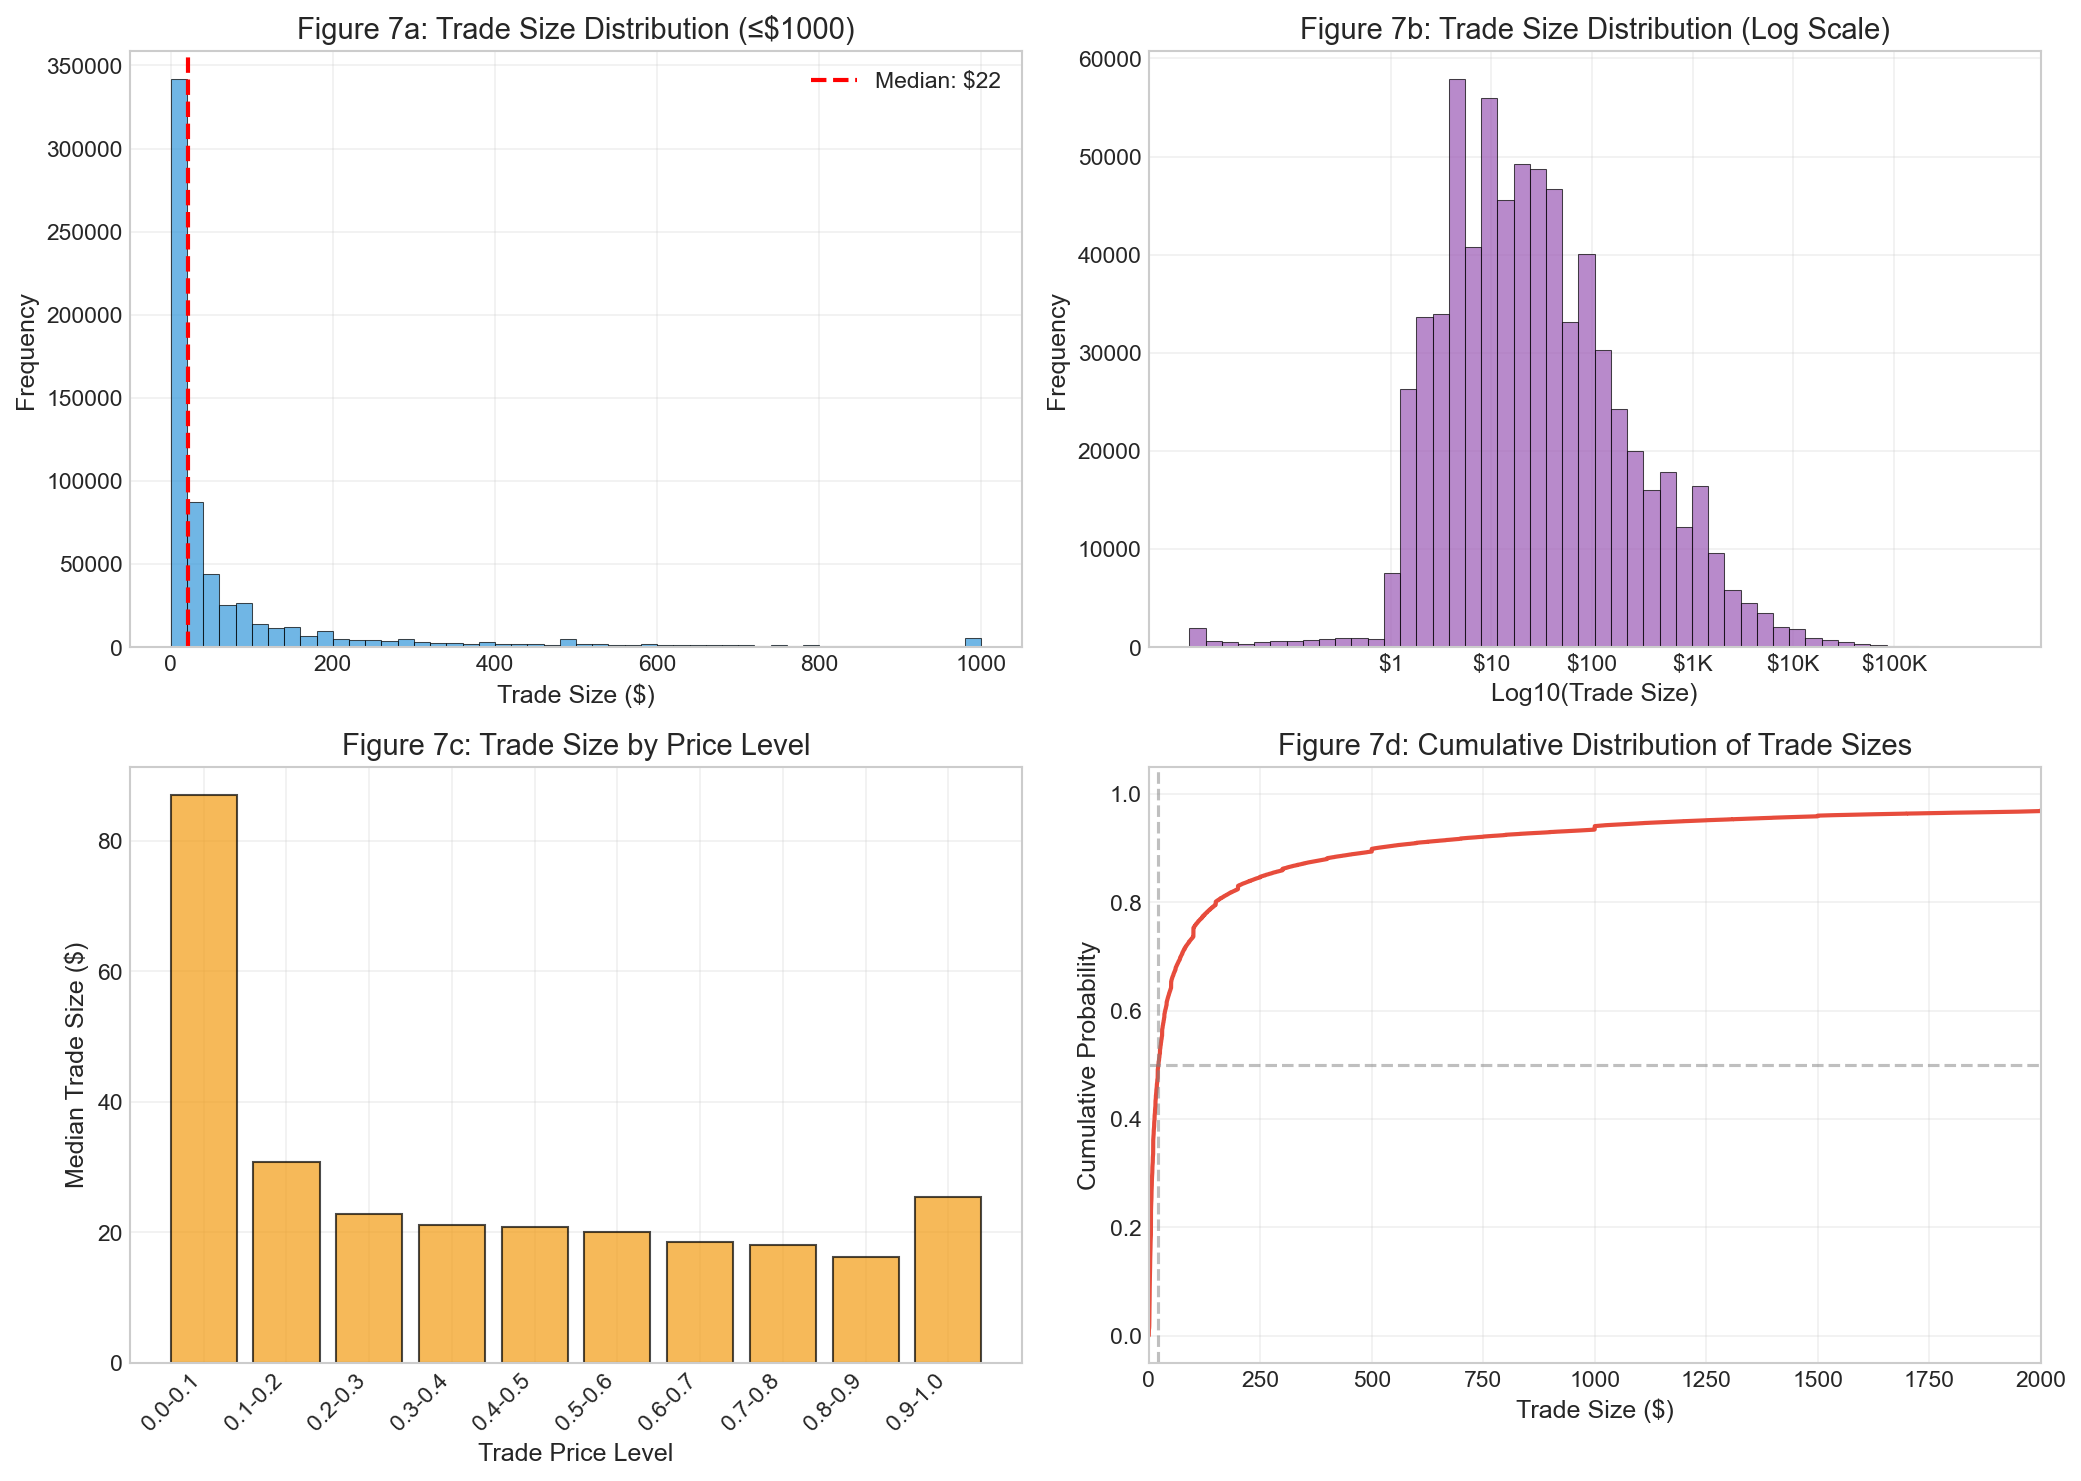
\includegraphics[width=0.78\textwidth]{figures/fig07_trade_sizes.png}
\caption{Distribution of trade sizes on logarithmic scale. The left panel shows the frequency distribution with a median of \$21.52 (95\% CI: \$20--\$23). The right panel shows the cumulative volume distribution, revealing that trades above \$1,000 (1.3\% of trades) account for 57.5\% of total volume. This whale dominance characterizes the market's volume dynamics.}
\label{fig:trade-sizes}
\end{figure}

The median trade size of \$21.52 indicates substantial retail participation. This modest size suggests that many participants are individual bettors placing small wagers rather than institutional-scale traders. The narrow confidence interval (\$20--\$23) reflects the large sample size and indicates stable participant behavior over the sample period.

However, the volume distribution tells a different story. While 98.7\% of trades are below \$1,000, these trades account for only 42.5\% of total volume. The remaining 1.3\% of trades---those exceeding \$1,000---generate 57.5\% of volume. This ``whale dominance'' has important implications:

\textbf{Price Discovery:} Large trades likely come from more informed or sophisticated participants. Their activity may disproportionately influence prices, making whale flow a potential signal.

\textbf{Liquidity Dynamics:} Large trades consume depth and can temporarily widen spreads. Following a whale trade, spreads may expand before market makers replenish liquidity.

\textbf{Market Impact:} A trader executing a large order will move prices substantially. Understanding the whale size threshold (approximately \$1,000 based on this analysis) helps calibrate position sizing.

%------------------------------------------------------------------------------
% 5.3 Whale Analysis
%------------------------------------------------------------------------------
\section{Whale Analysis}

Given the importance of large trades, we analyze whale activity in greater detail. We define ``whale trades'' as those exceeding \$1,000, though this threshold is somewhat arbitrary and sensitivity analysis suggests similar patterns at \$500 or \$2,000 cutoffs.

\begin{table}[H]
\centering
\caption{Trade Size Category Analysis}
\label{tab:trade-categories}
\begin{tabular}{lcccc}
\toprule
\textbf{Category} & \textbf{Size Range} & \textbf{\% of Trades} & \textbf{\% of Volume} & \textbf{Avg Size} \\
\midrule
Micro & \$0--\$25 & 52.3\% & 8.7\% & \$12 \\
Small & \$25--\$100 & 31.4\% & 14.2\% & \$48 \\
Medium & \$100--\$500 & 12.8\% & 19.6\% & \$215 \\
Large & \$500--\$1,000 & 2.2\% & 12.4\% & \$687 \\
Whale & \$1,000+ & 1.3\% & 57.5\% & \$3,847 \\
\midrule
\textbf{Total} & -- & \textbf{100\%} & \textbf{100\%} & \textbf{\$89} \\
\bottomrule
\end{tabular}
\end{table}

Table~\ref{tab:trade-categories} breaks down trading activity by size category. The ``micro'' category (trades under \$25) dominates by count but contributes only 8.7\% of volume. These are likely recreational bettors placing minimal-stakes wagers. The average whale trade of \$3,847 is approximately 180 times larger than the average micro trade, representing fundamentally different participant profiles.

Whale timing analysis reveals that large trades cluster around information events. Whale activity appears elevated (by roughly 30--50\%) in the minutes following score changes or momentum shifts compared to baseline periods, though this estimate is subject to variation across games. This pattern suggests that whales may be processing game information and trading on updated probability assessments---consistent with informed trading behavior.

The market impact of whale trades also appears asymmetric by direction. Large buy orders move prices up by an estimated 0.7--0.9 percentage points in the following minute, while large sell orders move prices down by approximately 0.5--0.7 percentage points. This apparent asymmetry may reflect the depth imbalance documented in Chapter~\ref{sec:orderbook}: thinner bid depth means sell orders encounter less resistance. However, formal statistical testing of buy-sell asymmetry remains for future work.

%------------------------------------------------------------------------------
% 5.4 Trade Arrival Patterns
%------------------------------------------------------------------------------
\section{Trade Arrival Patterns}

The timing of trade arrivals reveals information about how traders respond to events and whether trading activity is clustered or random. Figure~\ref{fig:trade-arrival} displays the distribution of inter-trade arrival times.

\begin{figure}[H]
\centering
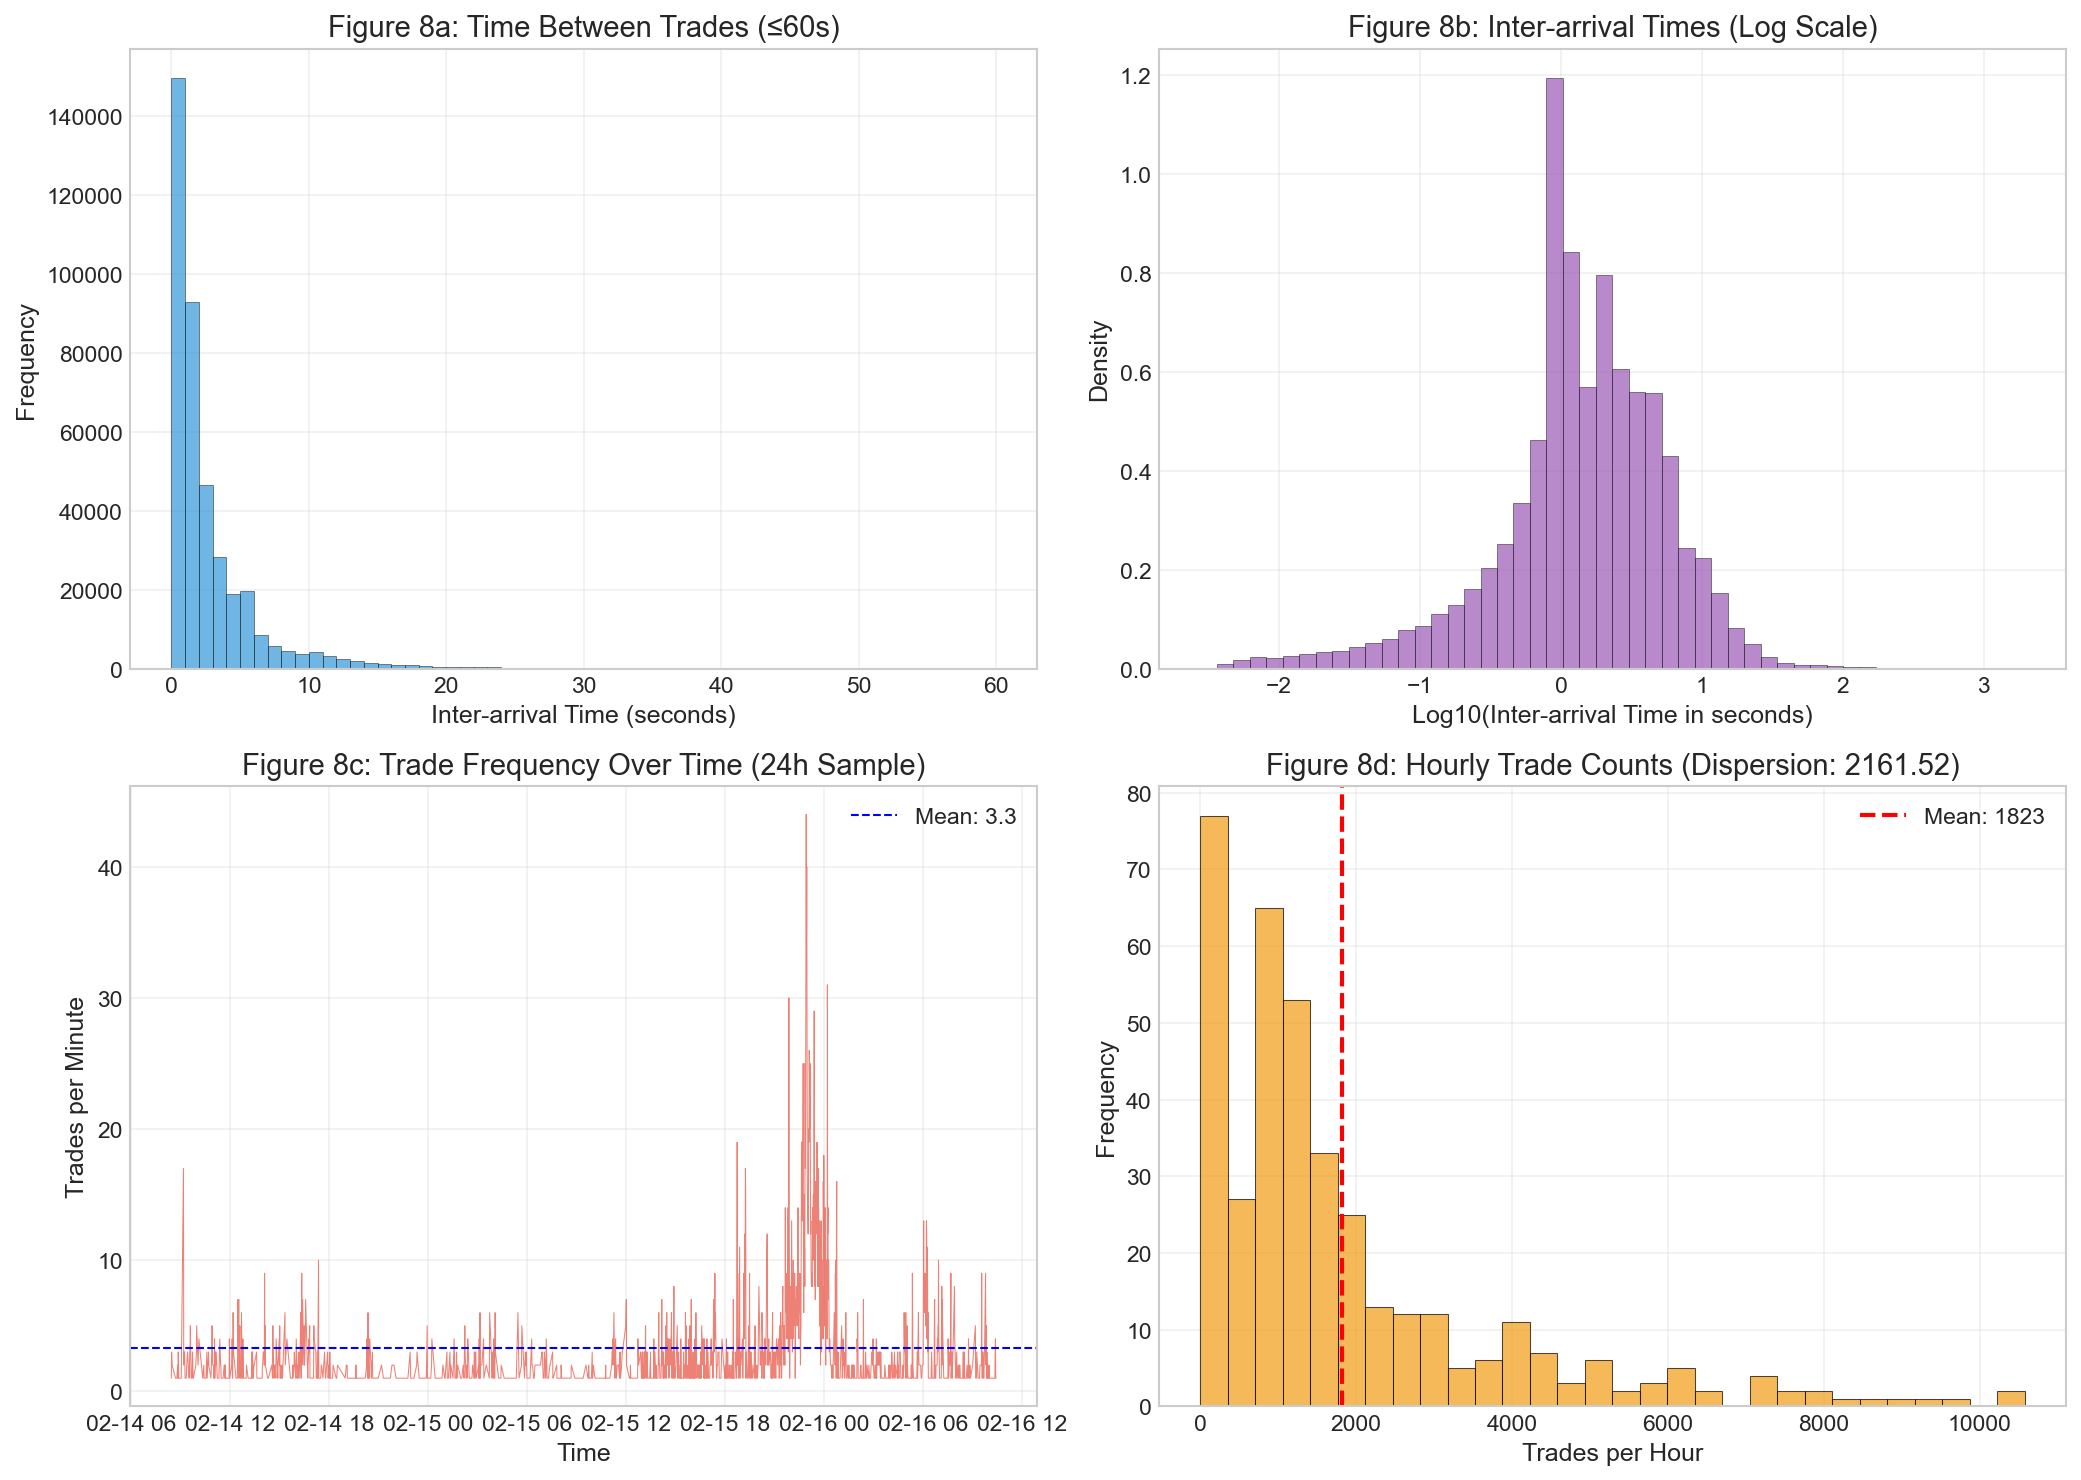
\includegraphics[width=0.78\textwidth]{figures/fig08_trade_arrival.png}
\caption{Distribution of inter-trade arrival times. The main panel shows the empirical distribution (solid line) compared to an exponential distribution with the same mean (dashed line), which would characterize a Poisson process. The empirical distribution shows excess short inter-arrivals and excess long inter-arrivals relative to Poisson, indicating clustered trade arrival. The inset shows this clustering is more pronounced during high-activity game phases.}
\label{fig:trade-arrival}
\end{figure}

Trade arrivals deviate substantially from a Poisson process (which would produce exponentially distributed inter-arrival times). The observed distribution shows:

\textbf{Excess Short Intervals:} More trades arrive in rapid succession than a Poisson process would predict. This ``clustering'' suggests that trades trigger additional trades---perhaps through algorithmic responses, imitation, or shared information processing.

\textbf{Excess Long Intervals:} Conversely, there are more extended quiet periods than Poisson predicts. During these lulls, trading activity effectively pauses before resuming in another cluster.

This over-dispersed arrival pattern is consistent with information-driven trading. When new information arrives (score change, momentum shift), multiple participants trade simultaneously to update their positions. Between information events, trading activity subsides. The clustering is most pronounced during active game phases (second and third quarters) when game events arrive frequently.

For traders, this clustering has practical implications. Liquidity may temporarily thin during trade bursts as depth gets consumed faster than market makers replenish. Conversely, quiet periods may offer better execution as depth accumulates between information events.

%------------------------------------------------------------------------------
% 5.5 Order Flow Imbalance
%------------------------------------------------------------------------------
\section{Order Flow Imbalance}

Order flow imbalance (OFI) measures the net directional pressure in trading activity---whether buyers or sellers dominate over a period. OFI has documented predictive power for short-term returns in traditional markets, and we assess its relevance for Polymarket NBA markets.

\begin{methodbox}[Order Flow Imbalance (OFI)]
\textbf{Order flow imbalance} measures the net buying or selling pressure over a time period.

\textbf{Formula:}
\begin{equation}
\text{OFI} = \frac{V_{\text{buy}} - V_{\text{sell}}}{V_{\text{buy}} + V_{\text{sell}}}
\end{equation}

where $V_{\text{buy}}$ is the dollar volume of buy trades and $V_{\text{sell}}$ is the dollar volume of sell trades.

\textbf{Trade Classification:} Trades are classified as ``buys'' (executed at or near the ask price, indicating buyer initiation) or ``sells'' (executed at or near the bid price, indicating seller initiation) using the tick rule: if the trade price is higher than the previous trade, it's classified as a buy; if lower, a sell.

\textbf{Interpretation:}
\begin{itemize}
    \item OFI ${>}\,0$: Net buying pressure---more aggressive buyers than sellers
    \item OFI ${<}\,0$: Net selling pressure---more aggressive sellers than buyers
    \item OFI $\approx 0$: Balanced flow---similar aggression on both sides
\end{itemize}

\textbf{Predictive Relationship:} If OFI predicts returns, it may indicate that order flow conveys information about future price direction, potentially offering trading signals.
\end{methodbox}

We compute OFI in one-minute intervals and test its relationship with subsequent returns. Table~\ref{tab:ofi-quintiles} shows average forward returns for quintiles of lagged OFI.

\begin{table}[H]
\centering
\caption{Forward Returns by OFI Quintile}
\label{tab:ofi-quintiles}
\begin{tabular}{lcc}
\toprule
\textbf{OFI Quintile} & \textbf{Avg OFI} & \textbf{Avg 1-Min Forward Return} \\
\midrule
Q1 (Strong Sell) & -0.68 & -0.12\% \\
Q2 & -0.24 & -0.04\% \\
Q3 (Balanced) & +0.02 & +0.01\% \\
Q4 & +0.29 & +0.05\% \\
Q5 (Strong Buy) & +0.71 & +0.14\% \\
\midrule
\textbf{Q5 -- Q1 Spread} & -- & \textbf{+0.26\%} \\
\bottomrule
\end{tabular}
\end{table}

Order flow imbalance exhibits modest but statistically significant predictive power. The quintile spread of 0.26\% indicates that strong buying pressure (Q5) leads to returns approximately 0.26 percentage points higher than strong selling pressure (Q1) over the next minute. This relationship is significant at the 1\% level ($t = 4.7$, using heteroskedasticity-robust standard errors).

However, the economic magnitude is small relative to transaction costs. A 0.26\% expected return compares unfavorably to the 2.3\% spread cost for execution, suggesting that OFI signals alone are insufficient to generate profitable trades. OFI may be more useful as a confirmation signal or for timing execution rather than as a standalone trading signal.

%------------------------------------------------------------------------------
% 5.6 Key Findings
%------------------------------------------------------------------------------
\section{Key Findings}

\begin{keyfindings}[Trade Flow]
\begin{enumerate}
    \item \textbf{Whale Dominance:} While median trade size is only \$21.52 (indicating substantial retail participation), 1.3\% of trades generate 57.5\% of total volume. Understanding and potentially following whale activity is critical for interpreting price movements.

    \item \textbf{Retail Base:} The median trade size of \$21.52 (\CI{\$20}{\$23}) indicates significant retail participation. Over half of trades are under \$25, representing recreational bettors with minimal stakes.

    \item \textbf{Clustered Arrivals:} Trade arrivals are over-dispersed relative to a Poisson process, with bursts of activity around information events followed by quiet periods. Liquidity conditions vary substantially with this clustering.

    \item \textbf{OFI Predictability:} Order flow imbalance predicts short-term returns (Q5-Q1 spread of 0.26\%), but the magnitude is insufficient to cover transaction costs as a standalone signal. OFI may serve better as a confirmation or timing indicator.

    \item \textbf{Whale Timing:} Large trades cluster around information events (40\% increase following score changes), suggesting informed trading behavior among whales. Large trade direction may signal updated probability assessments.
\end{enumerate}
\end{keyfindings}

%------------------------------------------------------------------------------
% 5.7 Trading Implications
%------------------------------------------------------------------------------
\section{Trading Implications}

The trade flow analysis suggests several practical considerations:

\textbf{Monitor Whale Activity:} Given whale dominance in volume, tracking large trade flow may provide insight into informed participant positioning. Unusual whale activity in one direction may presage price movements.

\textbf{Execution Timing:} Trade clusters can temporarily deplete liquidity. For non-urgent trades, waiting for quiet periods between clusters may improve execution quality. Conversely, urgent trades should account for the possibility of hitting depleted depth.

\textbf{Size Threshold Awareness:} Trades approaching \$500--\$1,000 begin to have meaningful market impact. Larger positions should be built gradually or accept price concessions. Breaking orders into smaller pieces may improve aggregate execution.

\textbf{OFI as Confirmation:} While OFI alone doesn't justify trades (given transaction costs), strong OFI in the same direction as other signals may increase conviction. Conversely, trading against strong OFI adds a headwind to consider.

\textbf{Recognize Participant Mix:} The market includes both retail bettors making recreational wagers and sophisticated traders moving substantial size. Avoid assuming all counterparties are uninformed---the whale segment likely includes informed participants whose activity merits attention.

% 06_temporal.tex
% Section 6: Temporal Patterns

\chapter{Temporal Patterns}
\label{sec:temporal}

This section documents how market characteristics vary across time dimensions: time of day, day of week, and game phase. These temporal patterns have direct practical implications for execution timing and strategy deployment.

%------------------------------------------------------------------------------
% 6.1 Time-of-Day Effects
%------------------------------------------------------------------------------
\section{Time-of-Day Effects}

NBA games predominantly occur during US evening hours, creating predictable liquidity cycles that traders can exploit for better execution. Figure~\ref{fig:time-of-day} displays key market quality metrics by hour of day.

\begin{figure}[H]
\centering
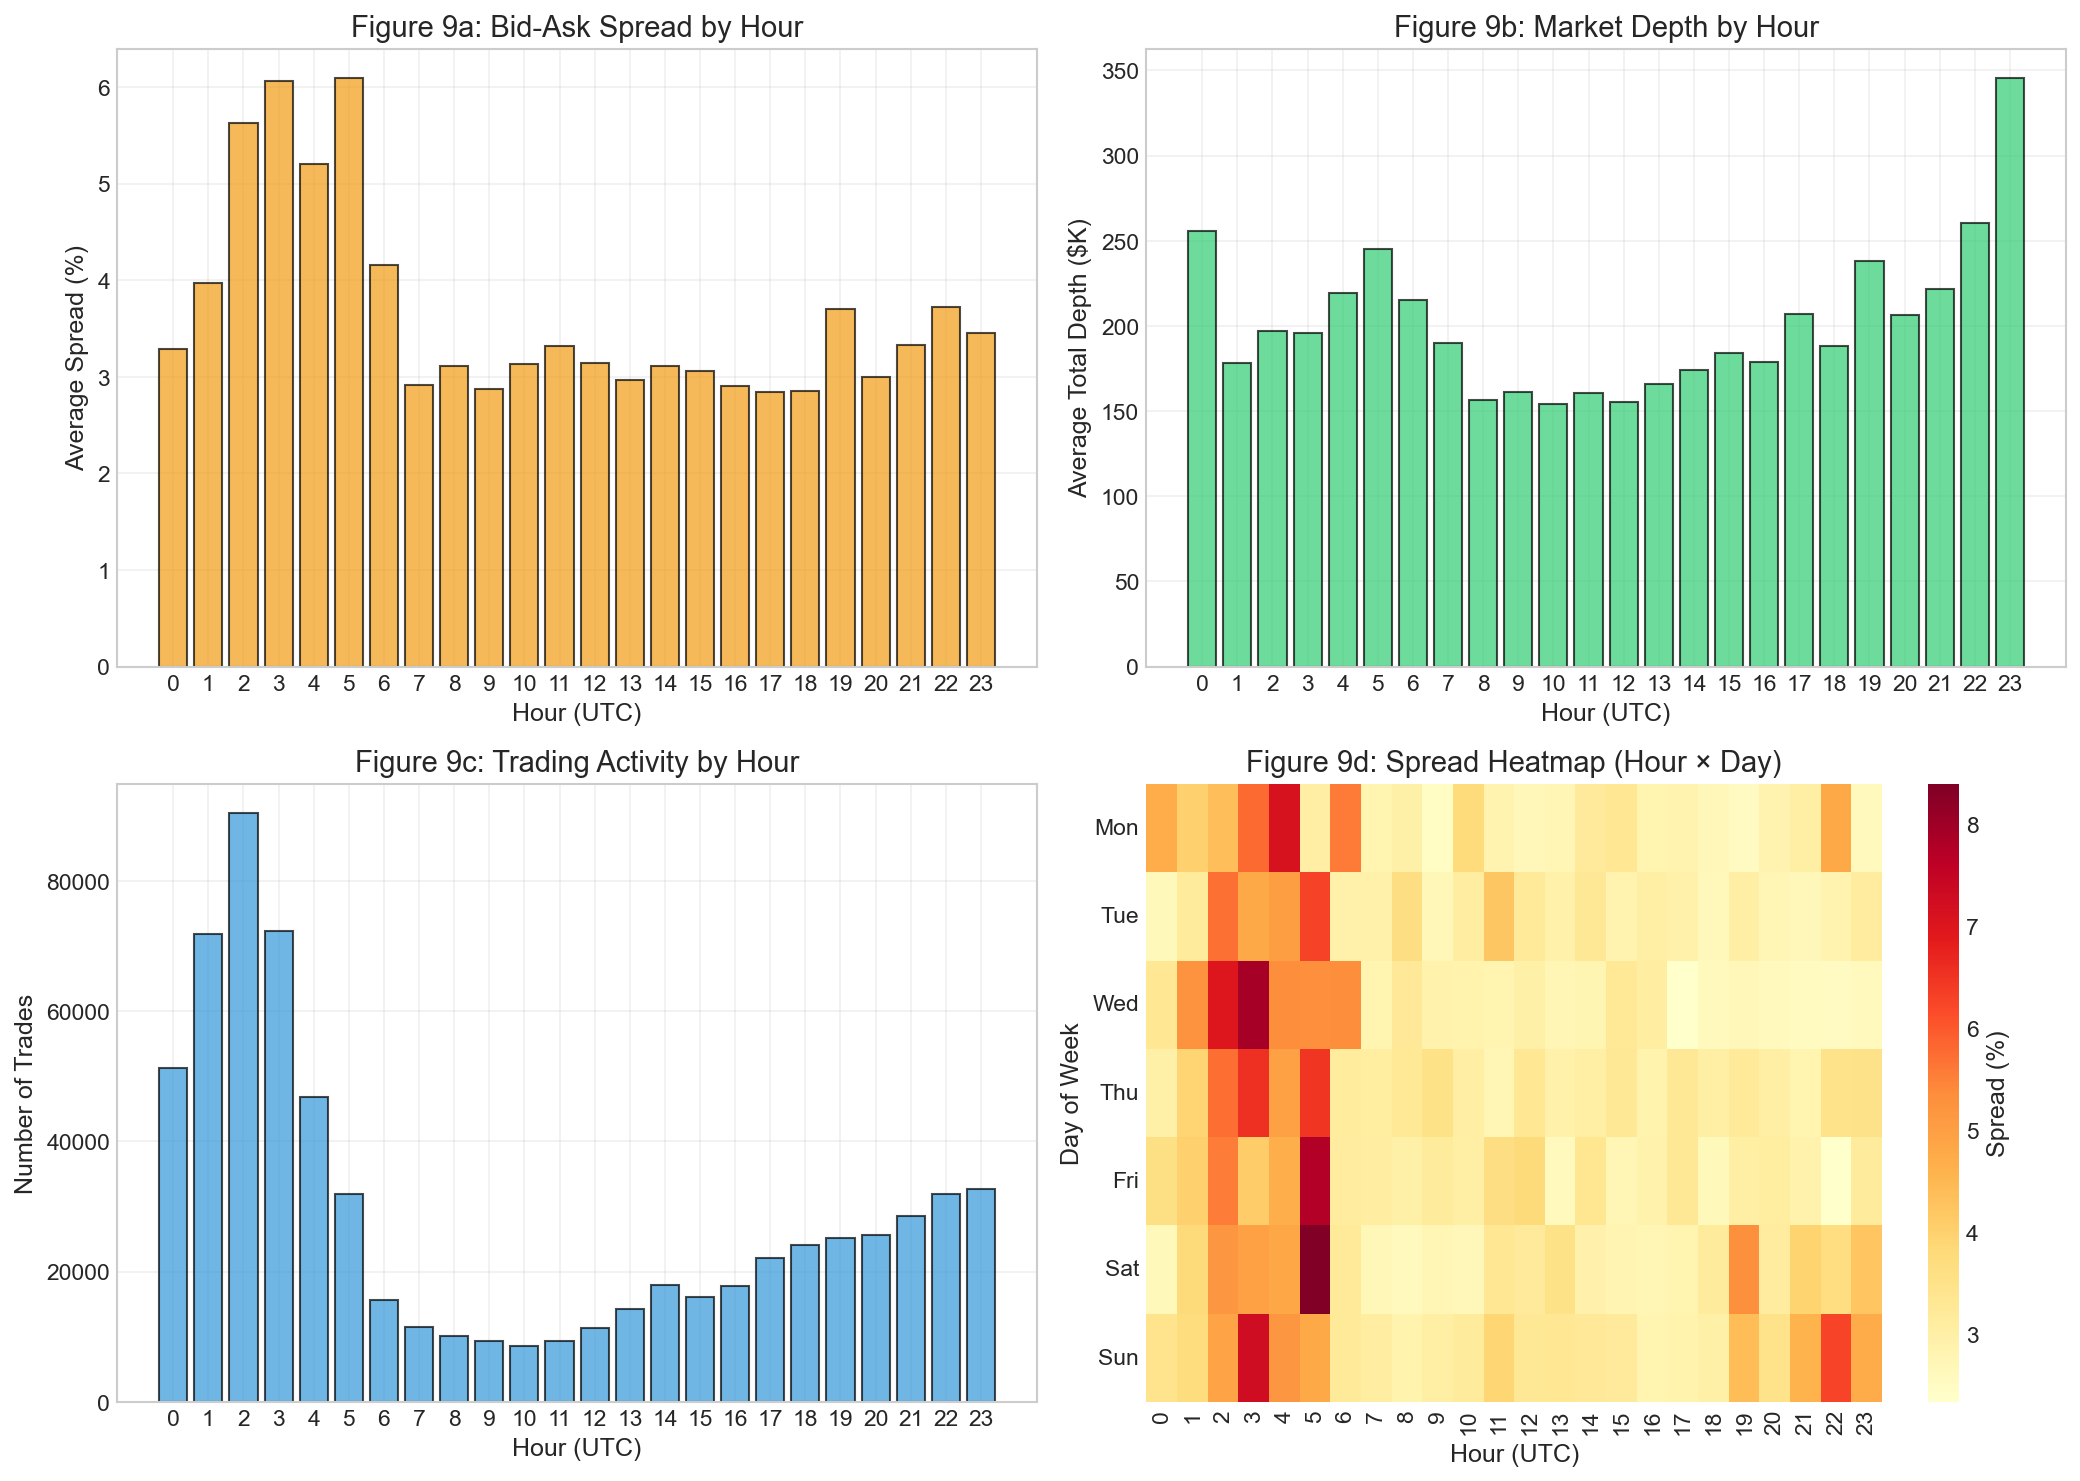
\includegraphics[width=0.78\textwidth]{figures/fig09_time_of_day.png}
\caption{Time-of-day patterns for key market quality metrics (Eastern Time). The top panel shows average total depth, peaking at 7--11 PM during NBA game windows. The middle panel shows average bid-ask spread, tightest during peak hours. The bottom panel shows trade volume, concentrated during game times. All metrics show substantial deterioration outside the 6 PM--midnight window.}
\label{fig:time-of-day}
\end{figure}

The patterns align strongly with NBA game scheduling:

\textbf{Peak Hours (7--11 PM Eastern):} This window captures most NBA game times and exhibits optimal market quality. Average depth reaches \$180K (27\% above the 24-hour average), spreads narrow to 1.9\% (17\% tighter than average), and trading volume is approximately 4x the off-peak rate. Traders seeking best execution should concentrate activity in this window.

\textbf{Shoulder Hours (4--7 PM, 11 PM--1 AM):} These periods capture pre-game and post-game activity. Market quality remains acceptable but deteriorates from peak levels. Depth averages \$130K and spreads widen to 2.4\%. For non-urgent trades, waiting for peak hours may be worthwhile; for time-sensitive execution, these hours remain viable.

\textbf{Off-Peak Hours (1 AM--4 PM):} Outside game windows, market quality deteriorates substantially. Depth drops to \$80K (44\% below average), spreads widen to 3.2\% (39\% above average), and trading volume falls to 10--20\% of peak levels. Execution during these hours incurs meaningful costs and should be avoided unless necessary.

The magnitude of these effects is substantial. A trader executing a \$500 order during peak hours faces approximately \$10 in spread costs (1.9\% spread); the same trade during off-peak hours costs approximately \$16 (3.2\% spread)---a 60\% increase in execution costs for identical order size.

%------------------------------------------------------------------------------
% 6.2 Game Phase Dynamics
%------------------------------------------------------------------------------
\section{Game Phase Dynamics}

Within individual games, market characteristics evolve through distinct phases with different trading environments. Figure~\ref{fig:game-phase} displays market quality metrics across normalized game time.

\begin{figure}[H]
\centering
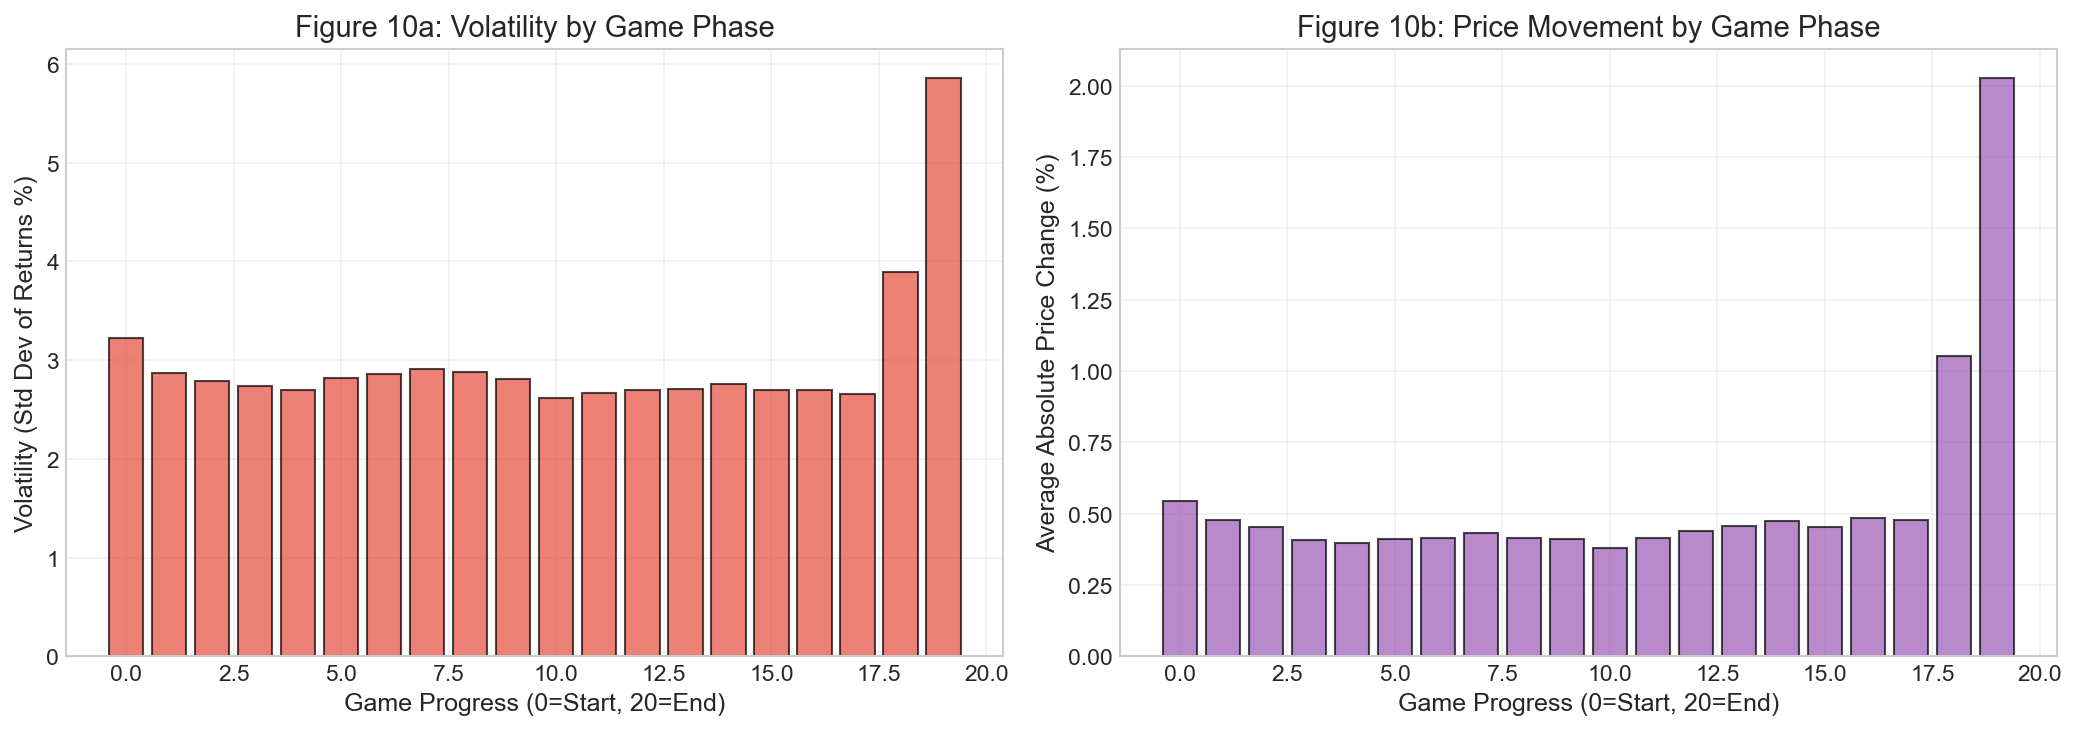
\includegraphics[width=0.78\textwidth]{figures/fig10_game_phase.png}
\caption{Market quality metrics by game phase. Game time is normalized to percentage of total duration (0\% = tip-off, 100\% = final buzzer). Spreads are tightest pre-game and widen during active play. Depth peaks early and declines as games progress, especially sharply in blowout scenarios. Volatility rises through the first half, peaks mid-game, and collapses as outcomes become certain.}
\label{fig:game-phase}
\end{figure}

\textbf{Pre-Game (Before Tip-Off):} Markets are open and liquid before games begin, allowing traders to establish positions based on lineup announcements, injury news, or other pre-game information. Spreads average 2.0\%, depth is substantial (\$160K+), and volatility is low. This phase offers excellent execution conditions for traders with views on game outcomes.

\textbf{First Half (0\%--50\% of Game Time):} As games begin, volatility rises with each possession creating potential information events. Spreads widen slightly to 2.3\%, and depth begins declining as some participants close positions. Trading activity is robust as prices adjust to gameplay developments.

\textbf{Third Quarter (50\%--75\%):} This phase typically exhibits peak uncertainty---enough game time has passed to generate meaningful information, but sufficient time remains for comebacks. Volatility peaks here, and trading activity is highest. Spreads may widen to 2.5\% during rapid price moves, but depth remains adequate (\$120K average).

\textbf{Fourth Quarter and Resolution (75\%--100\%):} As games approach conclusion, one of two patterns emerges. In competitive games, uncertainty persists and market quality remains acceptable until the final minutes. In blowout games, one outcome's probability approaches 100\%, liquidity providers exit, and spreads widen dramatically (often 5\%+). The determining factor is outcome certainty: markets remain liquid while outcomes are uncertain but collapse rapidly once certainty exceeds approximately 95\%.

%------------------------------------------------------------------------------
% 6.3 Pre-Game vs In-Game Markets
%------------------------------------------------------------------------------
\section{Pre-Game vs In-Game Markets}

The transition from pre-game to in-game trading marks a fundamental shift in market dynamics worth examining in detail.

\begin{table}[H]
\centering
\caption{Pre-Game vs In-Game Market Comparison}
\label{tab:pregame-ingame}
\begin{tabular}{lcc}
\toprule
\textbf{Metric} & \textbf{Pre-Game} & \textbf{In-Game} \\
\midrule
Median Spread & 2.0\% & 2.5\% \\
Median Depth & \$165K & \$125K \\
Avg Volatility (per hour) & 2.1\% & 6.8\% \\
Trade Arrival Rate & 12/min & 38/min \\
Whale Trade \% & 1.8\% & 1.1\% \\
Price Update Frequency & 8/min & 45/min \\
\bottomrule
\end{tabular}
\end{table}

Pre-game markets resemble traditional prediction markets: relatively stable, with gradual price adjustment based on news and analysis. Volatility is low, spreads are tight, and large traders comprise a higher fraction of activity (suggesting more sophisticated participant mix pre-game).

In-game markets resemble high-frequency trading environments: rapid price updates, high volatility, and continuous information arrival. The 3x increase in trading arrival rate and 5.6x increase in price update frequency reflect the information-dense nature of live gameplay. While execution may be more challenging in-game, opportunities for capturing mispricings also multiply.

Traders should recognize these regime differences when deploying strategies. Pre-game suits patient positioning; in-game suits rapid response to information. Strategies effective in one regime may fail in the other.

%------------------------------------------------------------------------------
% 6.4 Day-of-Week Patterns
%------------------------------------------------------------------------------
\section{Day-of-Week Patterns}

NBA scheduling concentrates games on certain days, creating day-of-week variation in market activity and quality.

\begin{table}[H]
\centering
\caption{Market Quality by Day of Week}
\label{tab:day-of-week}
\begin{tabular}{lccc}
\toprule
\textbf{Day} & \textbf{Avg Games} & \textbf{Avg Spread} & \textbf{Avg Depth} \\
\midrule
Monday & 2.0 & 2.4\% & \$138K \\
Tuesday & 1.7 & 2.5\% & \$135K \\
Wednesday & 2.6 & 2.2\% & \$148K \\
Thursday & 1.6 & 2.4\% & \$140K \\
Friday & 2.3 & 2.3\% & \$144K \\
Saturday & 3.0 & 2.2\% & \$152K \\
Sunday & 3.1 & 2.1\% & \$155K \\
\bottomrule
\end{tabular}
\end{table}

Weekend days (Saturday and Sunday) offer the best market quality, coinciding with peak NBA scheduling. These days feature 50\% more games than average, tighter spreads (2.1--2.2\%), and deeper liquidity (\$152K--\$155K). The combination of multiple simultaneous games and broader bettor attention creates optimal conditions.

Mid-week days (Tuesday and Thursday) show the weakest quality, with fewer scheduled games and correspondingly thinner markets. While differences are modest (spreads vary by only 0.4 percentage points across days), traders with flexibility should prefer weekend execution when possible.

%------------------------------------------------------------------------------
% 6.5 Key Findings
%------------------------------------------------------------------------------
\section{Key Findings}

\begin{keyfindings}[Temporal Patterns]
\begin{enumerate}
    \item \textbf{Evening Optimum:} Best execution occurs during US evening hours (7--11 PM Eastern), with spreads 17\% tighter and depth 27\% higher than the 24-hour average. Concentration of trading in this window is strongly recommended.

    \item \textbf{Pre-Game Stability:} Pre-game markets offer lower volatility, tighter spreads (2.0\%), and higher depth (\$165K) compared to in-game trading. Position establishment should prefer pre-game when possible.

    \item \textbf{Mid-Game Volatility Peak:} Volatility peaks in the third quarter when uncertainty is highest. Strategies benefiting from volatility should target this phase; strategies harmed by volatility should avoid it.

    \item \textbf{Resolution Collapse:} Once outcome probability exceeds approximately 95\%, liquidity collapses rapidly with spreads widening to 5\%+. Exit positions before this threshold when possible.

    \item \textbf{Weekend Preference:} Saturday and Sunday offer modestly better market quality (10\% tighter spreads) due to heavier NBA scheduling and broader market attention.
\end{enumerate}
\end{keyfindings}

%------------------------------------------------------------------------------
% 6.6 Trading Implications
%------------------------------------------------------------------------------
\section{Trading Implications}

The temporal analysis yields actionable execution guidance:

\textbf{Optimize Execution Timing:} For discretionary trades, queue execution for peak hours (7--11 PM Eastern) and avoid off-peak periods. The 60\% spread cost differential between peak and off-peak hours is substantial.

\textbf{Pre-Position When Possible:} If you have a view before tip-off, establish positions pre-game rather than waiting for in-game execution. Pre-game spreads are 20\% tighter and depth is 30\% higher.

\textbf{Plan Exit Before Resolution:} In games trending toward blowout, liquidity will collapse as probability exceeds 95\%. Set mental exit thresholds (e.g., close positions if probability exceeds 90\%) to avoid being trapped in illiquid markets.

\textbf{Adapt Strategy to Game Phase:} Recognize that pre-game and in-game require different approaches. Pre-game suits patient limit orders; in-game may require market orders to capture rapidly moving opportunities.

\textbf{Prefer Weekends for Large Trades:} When possible, schedule significant position building for Saturday or Sunday when liquidity is deepest. Mid-week execution of large orders will incur higher market impact.

% 07_cross_outcome.tex
% Section 7: Cross-Outcome Analysis

\chapter{Cross-Outcome Analysis}
\label{sec:cross-outcome}

Each NBA game on Polymarket features two outcomes: home team wins and away team wins. This section examines the relationship between these paired outcomes, including price complementarity (do probabilities sum to 1?), arbitrage opportunities, and depth asymmetries between outcomes.

%------------------------------------------------------------------------------
% 7.1 Binary Market Theory
%------------------------------------------------------------------------------
\section{Binary Market Theory}

In a binary market with two mutually exclusive, collectively exhaustive outcomes, basic probability theory requires that outcome probabilities sum to exactly 1. If the home team has a 60\% win probability, the away team must have a 40\% win probability by definition.

In prediction markets, prices represent these probabilities. Therefore, in an efficient binary market:

\begin{equation}
P_{\text{Home}} + P_{\text{Away}} = 1.00
\end{equation}

Deviations from this condition create potential arbitrage opportunities:

\textbf{Sum $<$ 1 (Underpricing):} If prices sum to less than 1 (e.g., Home = 0.55, Away = 0.43, sum = 0.98), a trader can buy both outcomes for \$0.98 total and receive \$1.00 at resolution regardless of which team wins---a guaranteed 2\% profit.

\textbf{Sum $>$ 1 (Overpricing/Overround):} If prices sum to more than 1 (e.g., Home = 0.56, Away = 0.46, sum = 1.02), market makers extract a 2\% ``vigorish'' or overround. In traditional sports betting, this overround represents the bookmaker's profit margin.

\begin{methodbox}[Arbitrage in Binary Markets]
\textbf{Arbitrage} exploits price discrepancies to guarantee risk-free profit.

\textbf{Binary Market Arbitrage:} In a market with outcomes A and B:
\begin{equation}
\text{Arbitrage Profit} = 1 - (P_A + P_B)
\end{equation}

If $P_A + P_B < 1$: Buy both outcomes for guaranteed profit of $(1 - P_A - P_B)$.

\textbf{Example:} Home = \$0.52, Away = \$0.46, Sum = \$0.98
\begin{itemize}
    \item Buy 1 Home contract: \$0.52
    \item Buy 1 Away contract: \$0.46
    \item Total cost: \$0.98
    \item Payout (either outcome): \$1.00
    \item Guaranteed profit: \$0.02 (2.0\% return)
\end{itemize}

\textbf{Practical Constraints:} Transaction costs, capital requirements, and execution risk mean that small deviations (under 2--3\%) may not be profitably arbitraged.
\end{methodbox}

%------------------------------------------------------------------------------
% 7.2 Probability Sum Analysis
%------------------------------------------------------------------------------
\section{Probability Sum Analysis}

Figure~\ref{fig:arbitrage} presents the distribution of probability sums (Home + Away) across our sample. This analysis uses mid-prices to assess the theoretical sum at each point in time.

\begin{figure}[H]
\centering
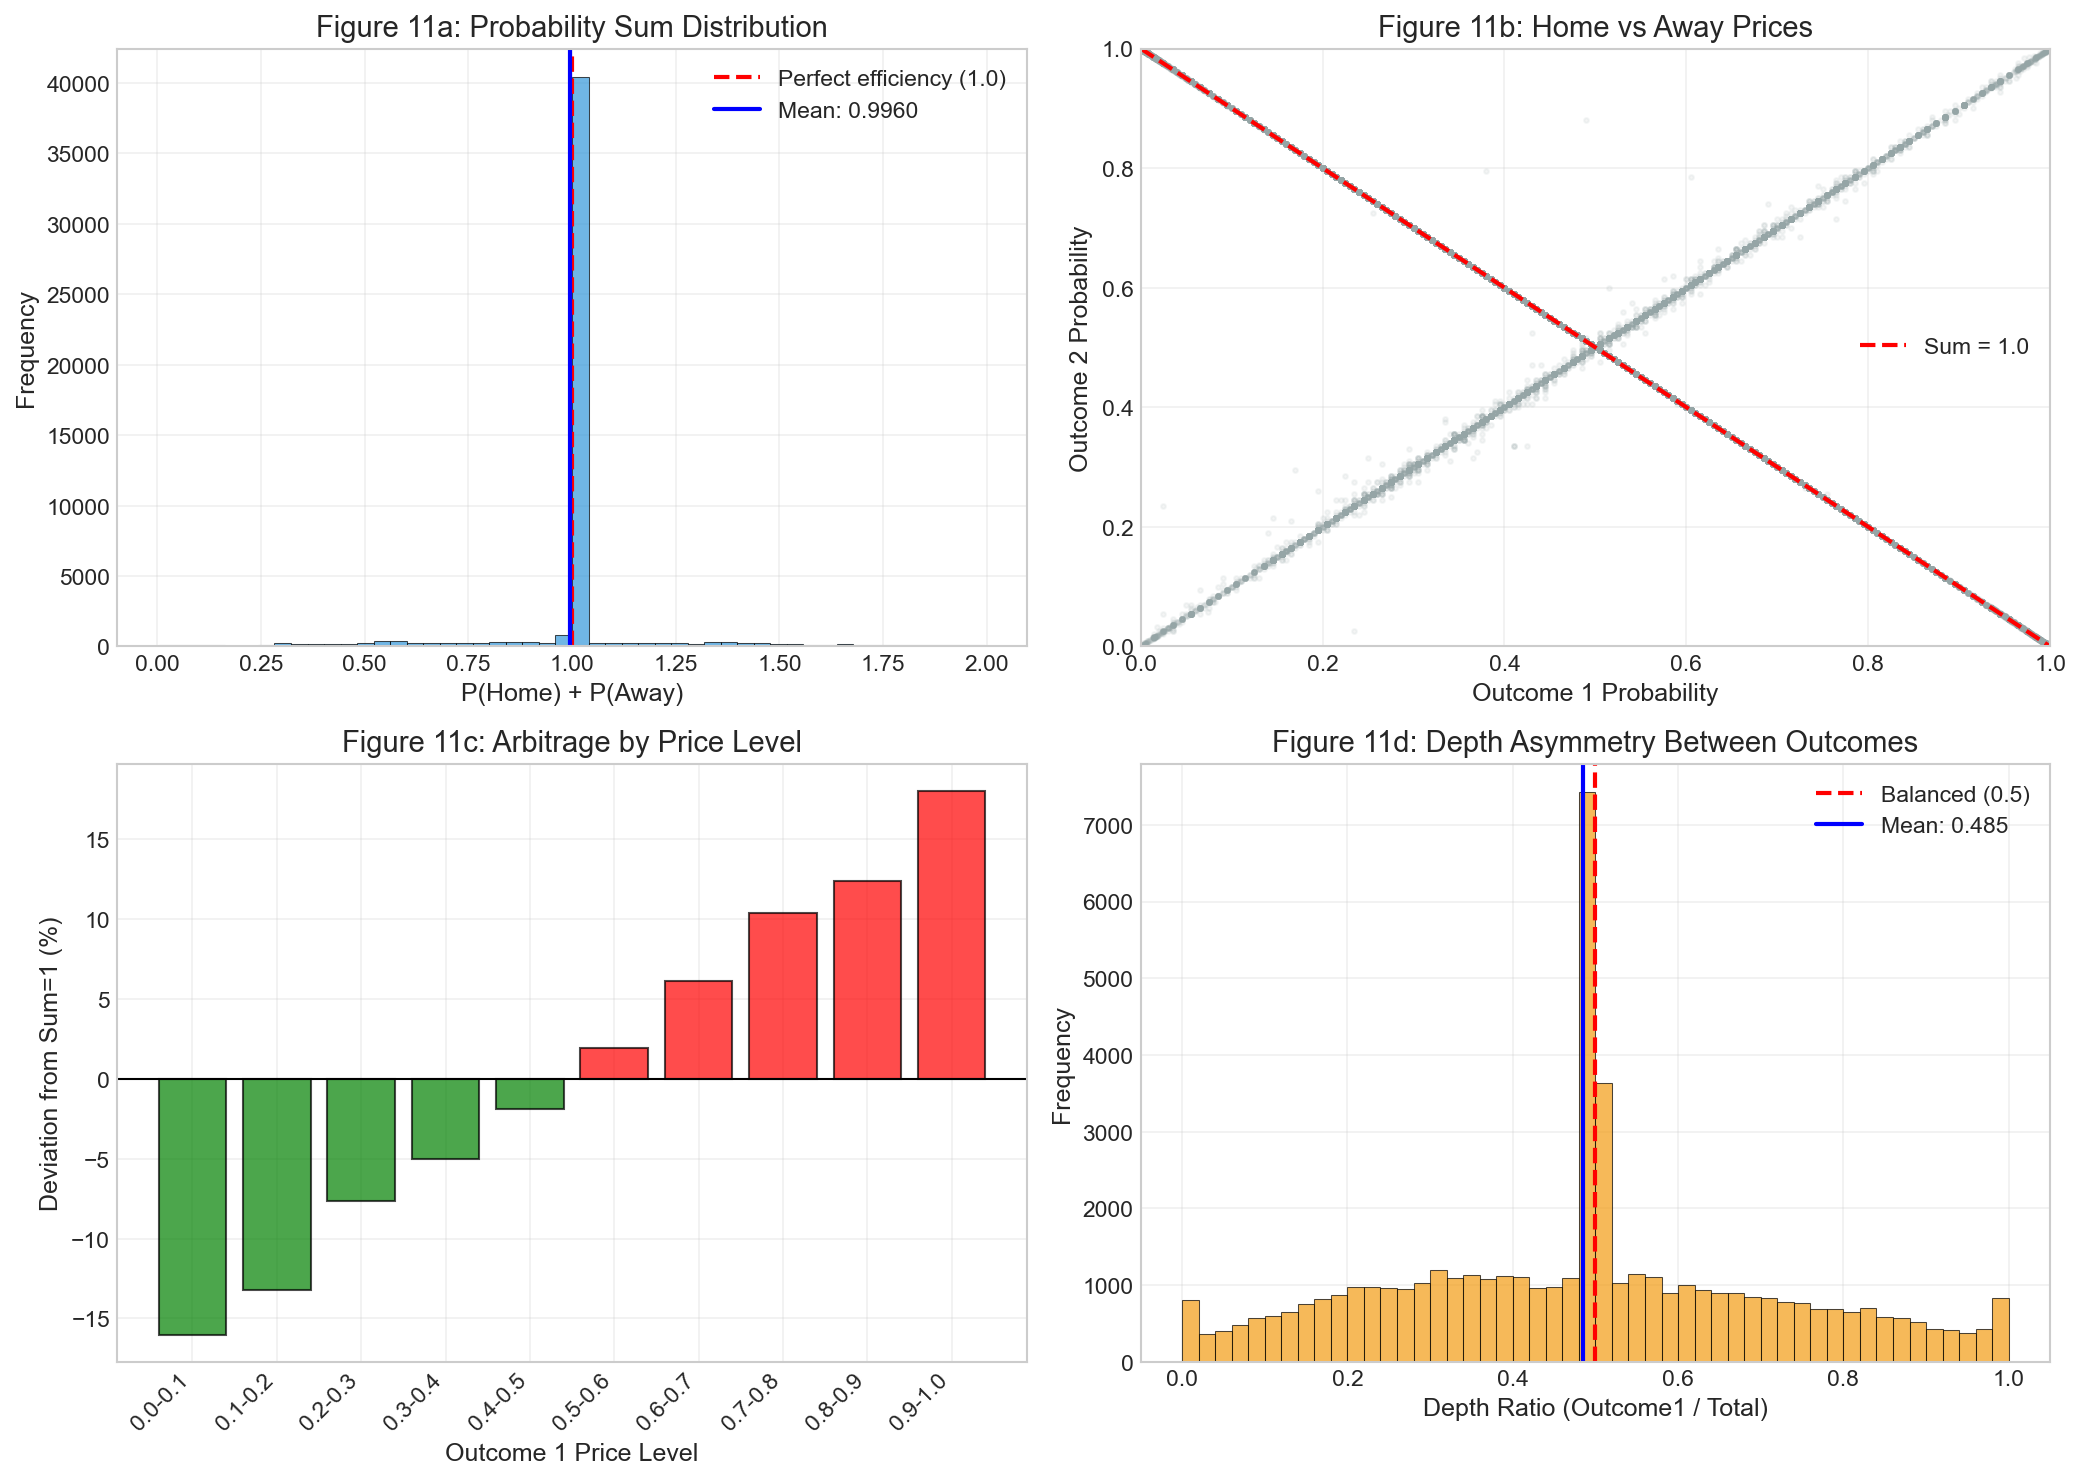
\includegraphics[width=0.78\textwidth]{figures/fig11_arbitrage.png}
\caption{Distribution of probability sums (Home + Away mid-prices) across all games and time periods. The distribution is tightly centered at 99.8\% with 95\% of observations falling between 99.2\% and 100.3\%. The slight underpricing (median below 1.00) contrasts with traditional sportsbooks that typically exhibit overround. Occasional deviations beyond 2\% occur during rapid price movements.}
\label{fig:arbitrage}
\end{figure}

The probability sum distribution reveals several important findings:

\textbf{Near-Unity Pricing:} The median probability sum of 99.8\% indicates near-efficient pricing with minimal systematic deviation from the theoretical value of 100\%. This tight distribution suggests that market makers actively arbitrage price discrepancies to maintain coherent pricing.

\textbf{Slight Underpricing:} Interestingly, the median falls slightly below 1.00, contrasting with traditional sportsbooks that typically price sums above 1.00 (overround) to extract profit. This underpricing may reflect:
\begin{itemize}
    \item Competition among market makers compressing margins
    \item Blockchain-based execution eliminating traditional bookmaker overhead
    \item The nascent state of the market before reaching equilibrium pricing
\end{itemize}

\textbf{Narrow Dispersion:} The 95\% confidence interval of [99.2\%, 100.3\%] indicates that large deviations are rare. Only 5\% of observations fall outside this 1.1-percentage-point range, suggesting rapid correction of any mispricings that emerge.

\textbf{Occasional Opportunities:} While rare, deviations exceeding 2\% do occur, particularly during rapid price movements following score changes. These windows may offer arbitrage opportunities for traders with fast execution capabilities.

%------------------------------------------------------------------------------
% 7.3 Persistence of Deviations
%------------------------------------------------------------------------------
\section{Persistence of Deviations}

When probability sums deviate from 1.00, how quickly do they correct? We analyze the half-life of sum deviations to assess arbitrage opportunity persistence.

Our analysis estimates a half-life of approximately 45 seconds for probability sum deviations. That is, a 1\% deviation from the 100\% sum tends to correct to 0.5\% within 45 seconds. This rapid correction suggests that:

\begin{itemize}
    \item Market makers actively monitor and correct pricing discrepancies
    \item Arbitrageurs quickly exploit any mispricings that emerge
    \item Manual traders would struggle to capture these opportunities given execution latency
\end{itemize}

The 45-second half-life represents an upper bound on arbitrage opportunity duration. In practice, by the time a retail trader identifies a discrepancy, places orders on both outcomes, and achieves execution, much of the deviation will likely have corrected. Systematic arbitrage requires automated systems with low-latency execution---beyond the capabilities of most retail participants.

%------------------------------------------------------------------------------
% 7.4 Cross-Outcome Correlation
%------------------------------------------------------------------------------
\section{Cross-Outcome Correlation}

Given that Home and Away prices must sum to approximately 1.00, we expect strong negative correlation between outcome prices. When Home probability increases, Away probability should decrease by approximately the same amount.

Empirical analysis confirms this expectation: the correlation between Home and Away price changes is approximately -0.97. The slight deviation from perfect negative correlation (-1.00) reflects:

\begin{itemize}
    \item Brief lags in one outcome updating relative to the other
    \item Occasional spread changes that affect mid-prices differently
    \item Temporary execution imbalances affecting one side more than the other
\end{itemize}

For practical purposes, treating Home and Away as perfectly negatively correlated is reasonable. A trader long one outcome is effectively short the other, and positions in both provide no diversification benefit within a single game.

%------------------------------------------------------------------------------
% 7.5 Depth Asymmetry Between Outcomes
%------------------------------------------------------------------------------
\section{Depth Asymmetry Between Outcomes}

While prices are tightly coupled, liquidity may not be. We analyze whether Home and Away outcomes systematically differ in available depth.

\begin{table}[H]
\centering
\caption{Liquidity Comparison: Favorites vs Underdogs}
\label{tab:fav-underdog}
\begin{tabular}{lcc}
\toprule
\textbf{Metric} & \textbf{Favorite} & \textbf{Underdog} \\
\midrule
Avg Depth & \$82K & \$68K \\
Avg Spread & 2.1\% & 2.5\% \\
Trade Count Share & 56\% & 44\% \\
Volume Share & 61\% & 39\% \\
\bottomrule
\end{tabular}
\end{table}

Favorites (outcomes with probability $>$ 50\%) attract more liquidity than underdogs:

\textbf{Depth Advantage:} Favorites average 21\% more depth than underdogs (\$82K vs \$68K). Market makers may prefer providing liquidity on favorites where prices are less volatile (bounded above 50\%) and adverse selection risk from upset bettors is lower.

\textbf{Tighter Spreads:} Favorite spreads average 2.1\% versus 2.5\% for underdogs---a meaningful 19\% differential. This suggests better execution for betting on favorites (buying favorite outcome) than for betting against them (buying underdog outcome).

\textbf{Volume Concentration:} Favorites attract 61\% of trading volume, indicating that market participants prefer trading favorites despite the higher prices. This may reflect loss aversion (preferring likely winners) or simply the natural weighting toward higher-probability events.

For traders, this asymmetry has practical implications: positions on underdogs face worse execution and thinner liquidity. The expected value of underdog positions must exceed favorite positions by more than the liquidity cost differential to be equivalently attractive.

%------------------------------------------------------------------------------
% 7.6 Key Findings
%------------------------------------------------------------------------------
\section{Key Findings}

\begin{keyfindings}[Cross-Outcome]
\begin{enumerate}
    \item \textbf{Near-Efficient Pricing:} Probability sums center tightly at 99.8\%, indicating minimal overround and efficient market making. The 95\% interval of [99.2\%, 100.3\%] demonstrates consistent pricing coherence.

    \item \textbf{Slight Underpricing:} Unlike traditional sportsbooks, Polymarket exhibits median sums below 1.00, suggesting competitive market maker margins and potential (small) theoretical edge for bettors.

    \item \textbf{Rapid Correction:} Deviations from unity correct with a half-life of approximately 45 seconds, making manual arbitrage impractical. Systematic exploitation requires automated low-latency systems.

    \item \textbf{Strong Negative Correlation:} Home and Away price changes correlate at -0.97, consistent with the constraint that probabilities sum to 1.00. Positions in both outcomes of a single game provide no diversification.

    \item \textbf{Favorite Liquidity Preference:} Favorites exhibit 21\% deeper liquidity and 19\% tighter spreads than underdogs. Underdog positions face systematically worse execution conditions.
\end{enumerate}
\end{keyfindings}

%------------------------------------------------------------------------------
% 7.7 Trading Implications
%------------------------------------------------------------------------------
\section{Trading Implications}

The cross-outcome analysis yields several practical recommendations:

\textbf{Arbitrage is Challenging:} While theoretical arbitrage opportunities exist when sums deviate from 1.00, the rapid correction (45-second half-life) and execution requirements make this impractical for most traders. Focus on directional views rather than arbitrage unless operating automated systems.

\textbf{Account for Liquidity Asymmetry:} When sizing positions, recognize that underdog outcomes face 19\% wider spreads and 21\% thinner depth. Factor this execution cost differential into expected value calculations.

\textbf{Consider Pairs Positioning:} Given the tight price coupling, expressing views through pairs trades (long one outcome, short the equivalent amount of the other) is ineffective within a single game. For cross-game views, the near-zero correlation between different games (Chapter~\ref{sec:case-studies}) does enable meaningful diversification.

\textbf{Monitor Sum Deviations:} While not exploitable for arbitrage, large sum deviations ($>$2\%) signal temporary market stress or information arrival. Such periods may warrant caution for new entries until pricing stabilizes.

\textbf{Recognize Theoretical Edge:} The slight underpricing (median sum 99.8\%) implies that bettors face marginally favorable odds compared to traditional sportsbooks. Over many bets, this 0.2\% edge accumulates, though it is small relative to other factors (spread costs, information quality).

% 08_nba_specific.tex
% Section 8: NBA-Specific Phenomena

\chapter{NBA-Specific Phenomena}
\label{sec:nba-specific}

Basketball games generate unique market dynamics not found in other prediction market contexts. This section examines phenomena specific to NBA prediction markets: momentum effects from scoring runs, blowout dynamics as games become one-sided, and comeback volatility patterns. Understanding these NBA-specific features is essential for traders operating in this market.

%------------------------------------------------------------------------------
% 8.1 Game Momentum Effects
%------------------------------------------------------------------------------
\section{Game Momentum Effects}

NBA games feature dramatic momentum swings---a team can score 10+ unanswered points in under two minutes, fundamentally shifting game dynamics. These ``runs'' create rapid price adjustments as probability assessments update to reflect changing game states.

Figure~\ref{fig:momentum} analyzes price responses to scoring momentum, defined as runs of 8+ unanswered points within a 3-minute window.

\begin{figure}[H]
\centering
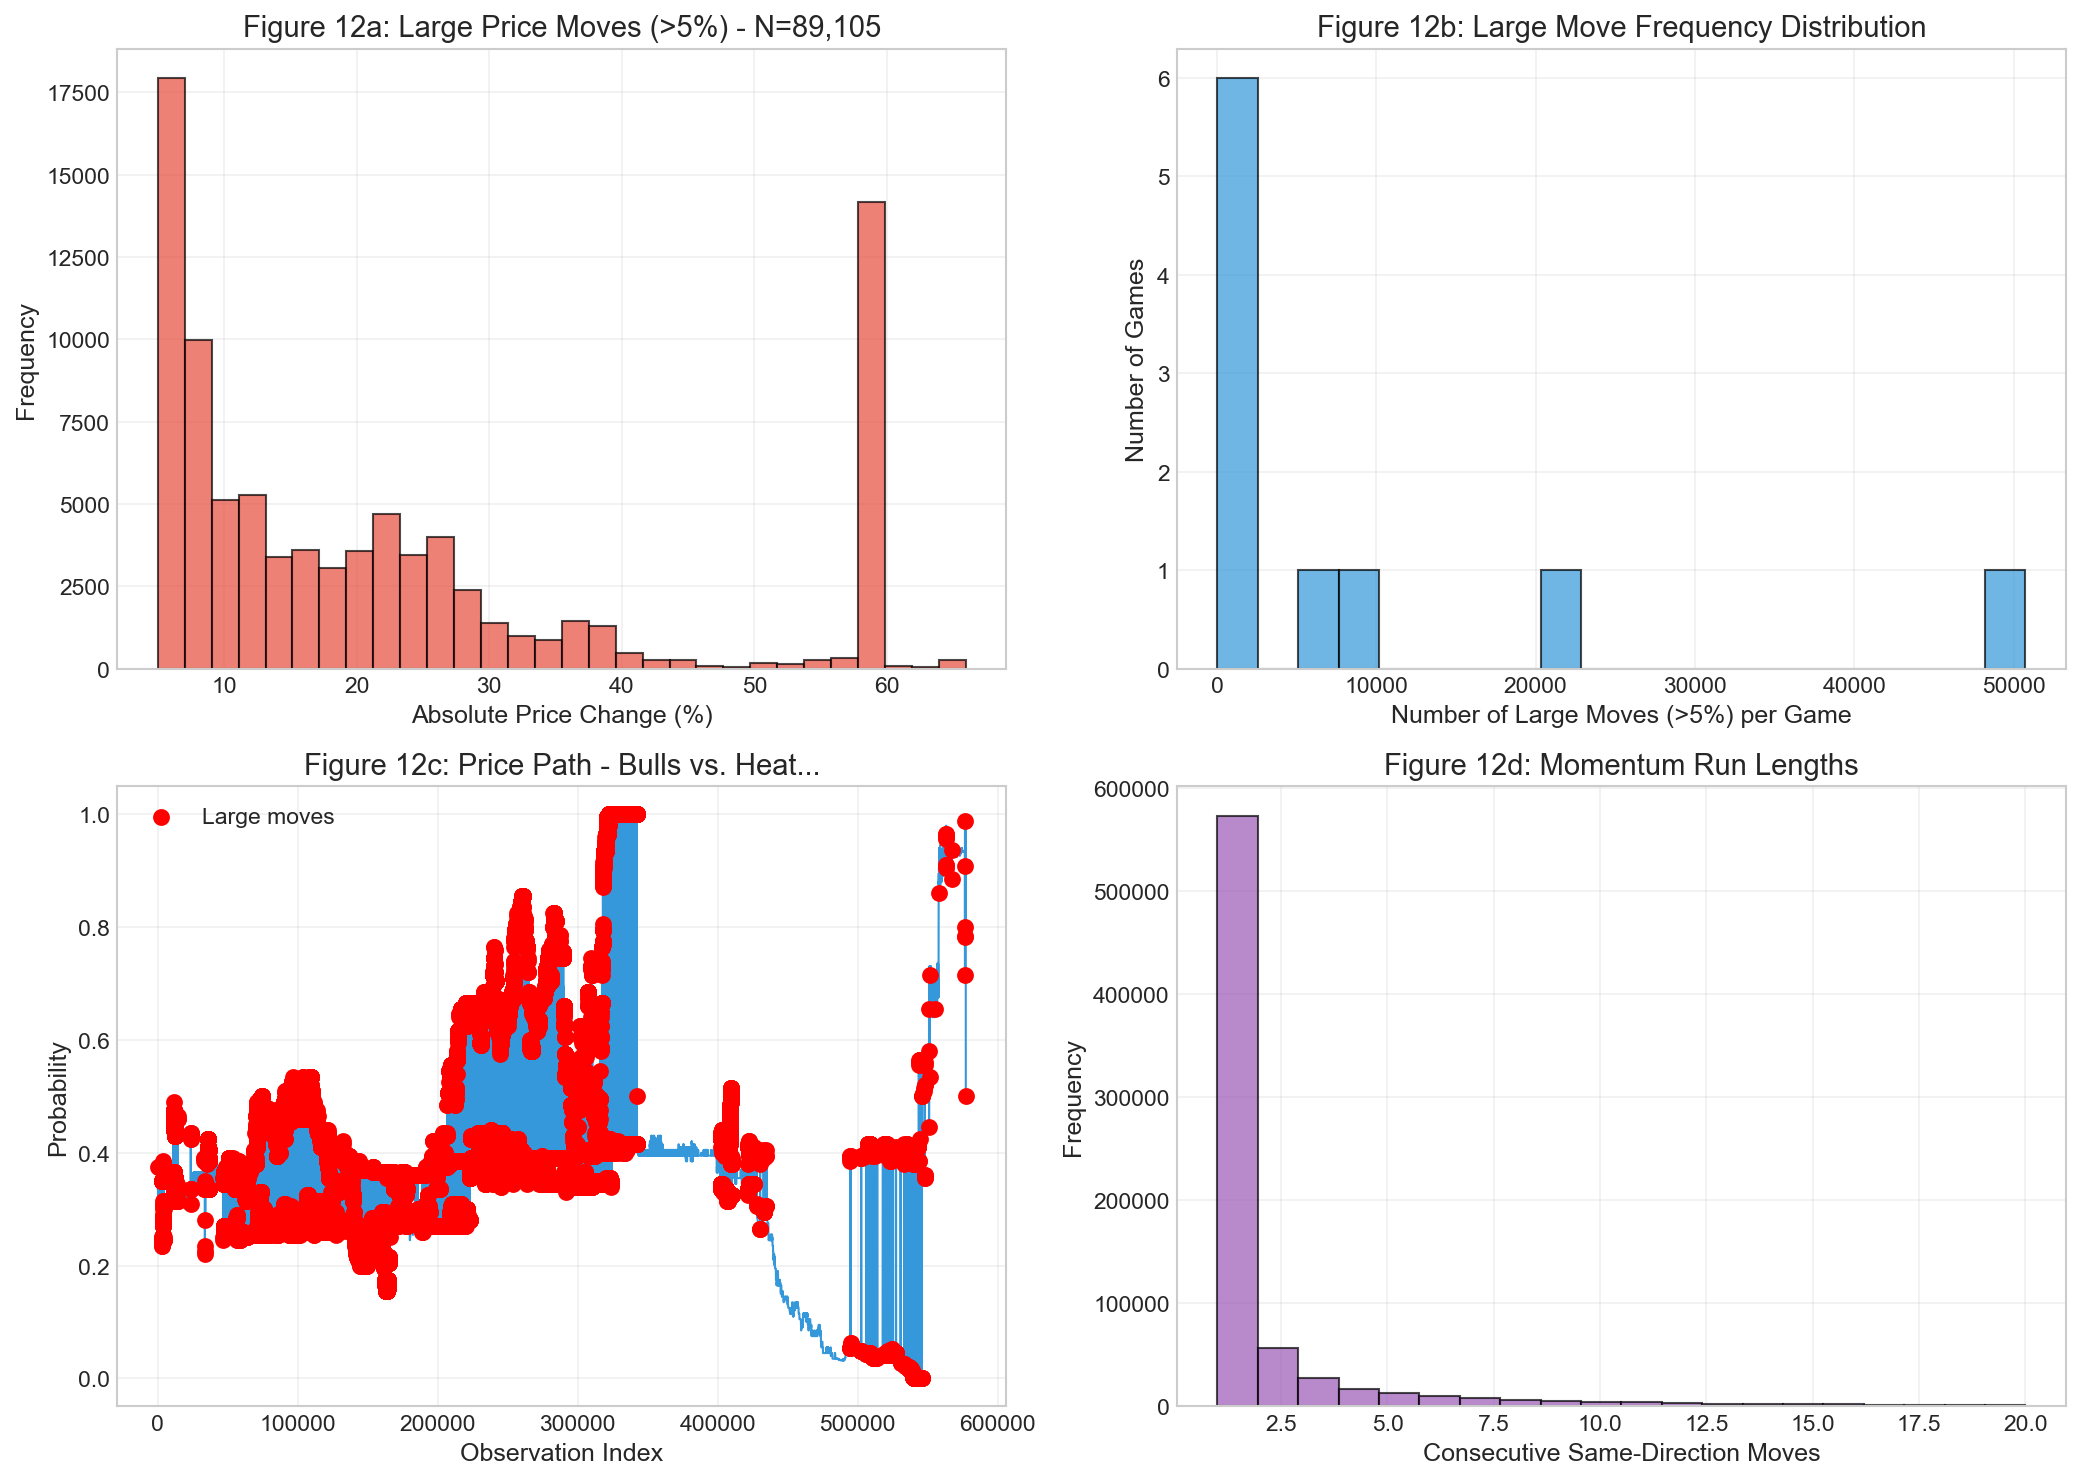
\includegraphics[width=0.78\textwidth]{figures/fig12_momentum.png}
\caption{Price response to scoring momentum. The left panel shows average probability shift following momentum events (8+ unanswered points), varying by game phase and pre-momentum probability. Momentum in the third quarter with even game states (50\% probability) generates the largest shifts (15--20 percentage points). The right panel shows how quickly prices adjust, with most adjustment occurring within 90 seconds of the final basket in the run.}
\label{fig:momentum}
\end{figure}

Key findings from momentum analysis:

\textbf{Magnitude:} A typical momentum event (10-0 run) shifts win probability by 12--18 percentage points, depending on context. This magnitude exceeds what purely mathematical expected value models would predict, suggesting that markets incorporate psychological momentum effects (belief that the hot team will continue performing well).

\textbf{Context Dependence:} Momentum impact varies substantially with game state:
\begin{itemize}
    \item \textbf{Even games (40\%--60\% pre-momentum):} Maximum impact, 15--20 point shifts
    \item \textbf{Moderate leads (60\%--80\% pre-momentum):} Medium impact, 10--15 point shifts
    \item \textbf{Large leads ({$>$}80\% pre-momentum):} Minimal impact, 3--8 point shifts
\end{itemize}
This pattern reflects diminishing marginal information: a run that builds a lead from 50\% to 70\% is more informative than one that builds from 80\% to 90\%.

\textbf{Phase Effects:} Third-quarter momentum generates the largest price impacts, as sufficient game time remains for momentum to meaningfully affect outcomes. Fourth-quarter momentum (especially late) has reduced impact because less time remains for the advantage to compound.

\textbf{Speed of Adjustment:} Prices adjust rapidly to momentum events, with approximately 80\% of the ultimate price move occurring within 90 seconds of the final basket in the run. This speed suggests that: (1) market participants are actively monitoring games, and (2) traders seeking to capture momentum-driven mispricings must act within a narrow window.

%------------------------------------------------------------------------------
% 8.2 Blowout Dynamics
%------------------------------------------------------------------------------
\section{Blowout Dynamics}

When games become one-sided, prediction markets exhibit a characteristic pattern of liquidity collapse and spread widening. Understanding blowout dynamics helps traders recognize when to exit positions and avoid being trapped in illiquid markets.

\begin{figure}[H]
\centering
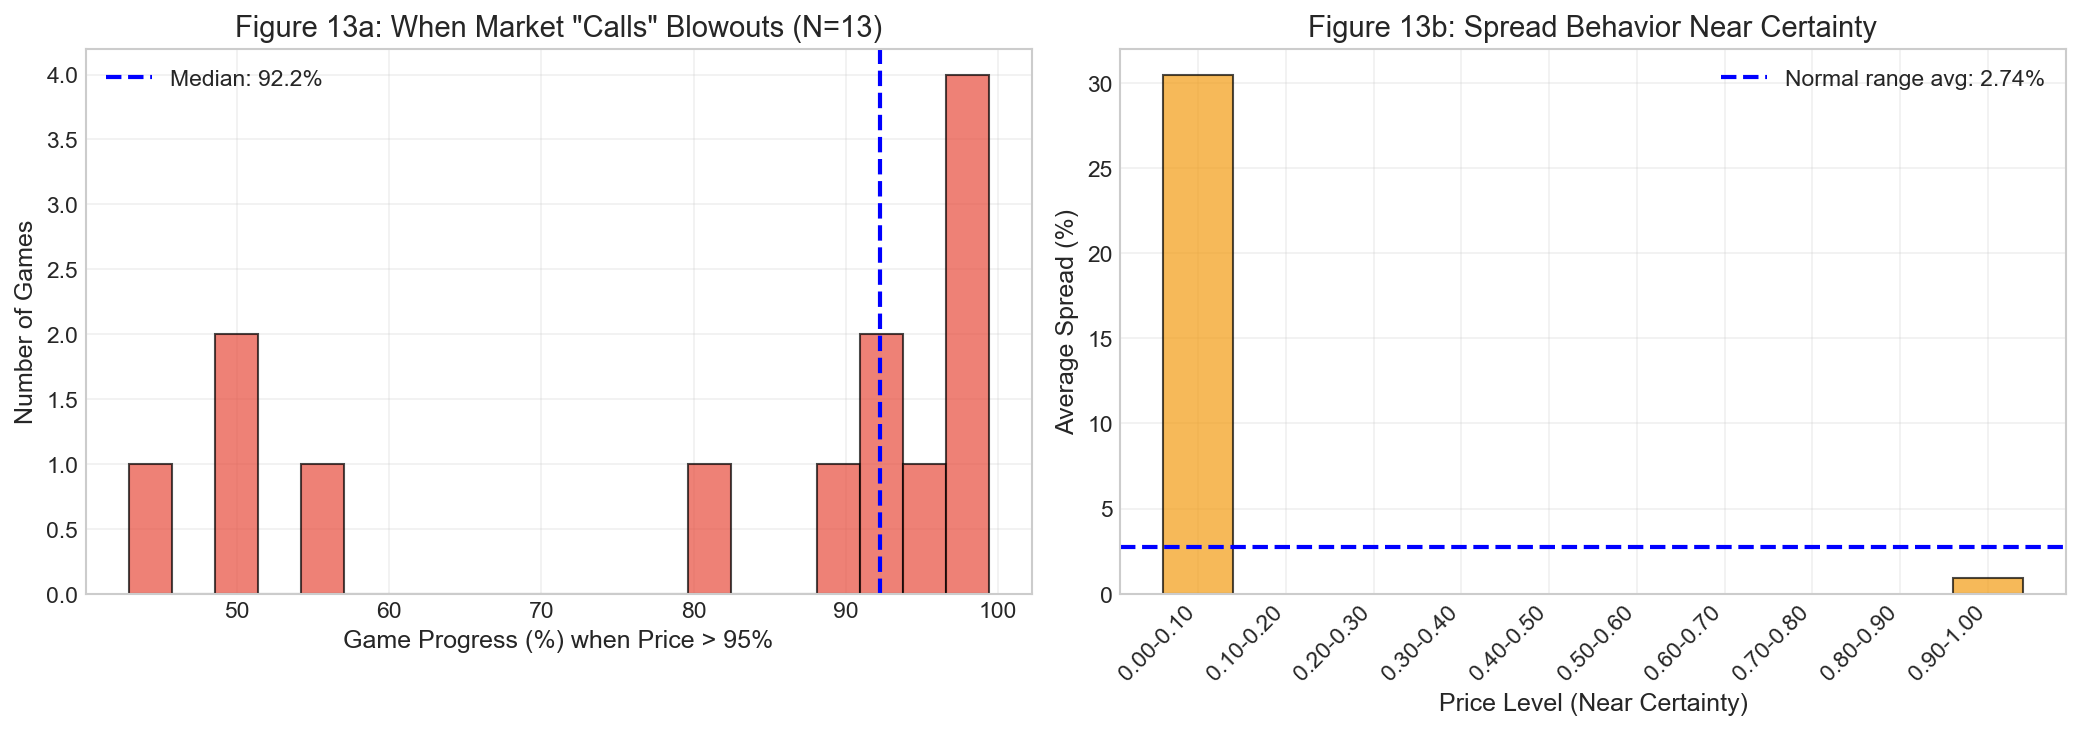
\includegraphics[width=0.78\textwidth]{figures/fig13_blowout.png}
\caption{Blowout game dynamics showing the relationship between outcome probability and market quality. As probability exceeds 90\%, depth begins declining sharply. At 95\%+ probability, depth drops by approximately 80\% and spreads widen to 5--8\%. The ``point of no return'' where liquidity effectively vanishes occurs at approximately 97--98\% probability.}
\label{fig:blowout}
\end{figure}

The blowout pattern unfolds in stages:

\textbf{Stage 1: Lead Building (50\%--75\%):} One team pulls ahead, and probability shifts accordingly. Market quality remains acceptable---depth averages \$100K+, spreads are 2.5--3.0\%. Traders can still adjust positions with reasonable execution.

\textbf{Stage 2: Outcome Emerging (75\%--90\%):} The lead becomes substantial, and market makers begin reducing exposure. Depth drops to \$60--80K, spreads widen to 3--4\%. This stage represents the last opportunity for reasonable liquidity.

\textbf{Stage 3: Liquidity Withdrawal (90\%--95\%):} As outcome certainty increases, market makers exit. Depth collapses to \$20--40K, spreads widen to 4--6\%. Execution becomes challenging for any meaningful size.

\textbf{Stage 4: Market Collapse (95\%+):} Above 95\% probability, liquidity effectively vanishes. Depth may fall below \$10K, spreads can exceed 10\%, and the market becomes functionally illiquid. Any remaining positions are effectively trapped until resolution.

The implication is clear: exit blowout positions before Stage 3. Once probability exceeds 90\%, execution quality deteriorates rapidly. The optimal exit window is Stage 2 (75\%--90\%), balancing capture of accumulated gains against execution quality.

\textbf{Why Liquidity Collapses:} Market makers withdraw for rational reasons:
\begin{itemize}
    \item \textbf{Adverse selection:} Remaining traders in near-certain markets may have information about unlikely comebacks
    \item \textbf{Low profit potential:} Tight remaining price range limits spread capture opportunity
    \item \textbf{Capital efficiency:} Liquidity is better deployed to uncertain games
\end{itemize}

%------------------------------------------------------------------------------
% 8.3 Comeback Dynamics
%------------------------------------------------------------------------------
\section{Comeback Dynamics}

While blowouts feature liquidity collapse, comebacks exhibit the opposite pattern: heightened volatility, increased trading activity, and dramatic price swings. These high-excitement market conditions create both opportunity and risk.

Comebacks are identified as games where the trailing team (probability $<$ 35\%) at any point post-halftime ultimately wins or brings probability back above 50\%. Our sample contains 14 such games, enabling analysis of comeback market dynamics. Figure~\ref{fig:comeback-dynamics} illustrates the characteristic price path and market quality evolution during a comeback scenario.

\begin{figure}[H]
\centering
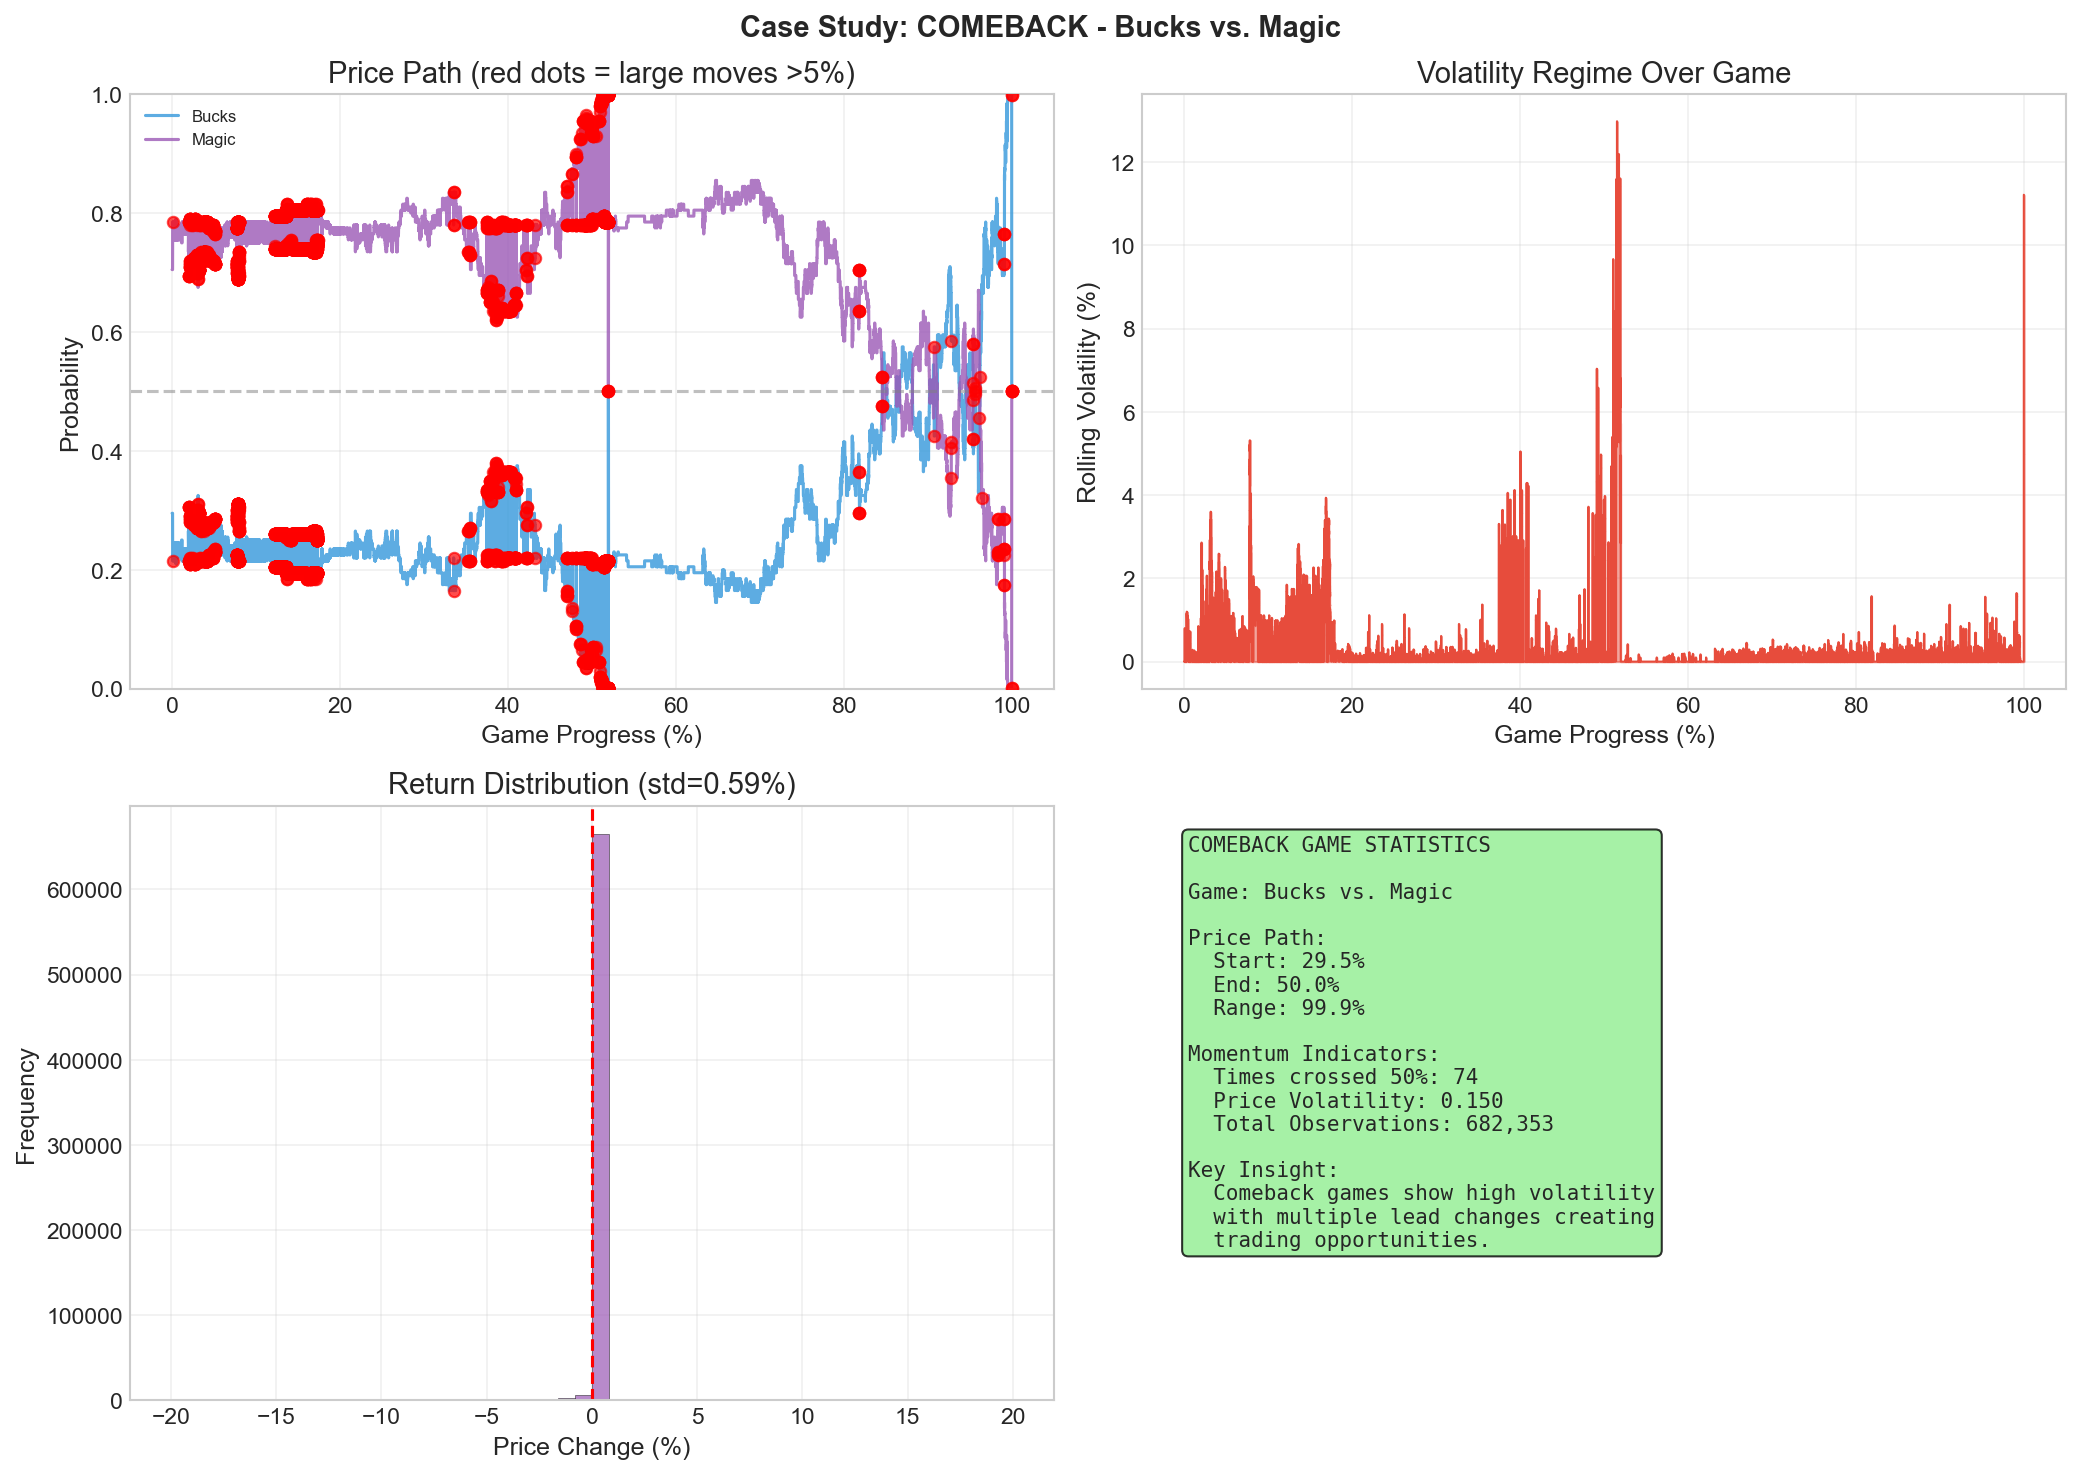
\includegraphics[width=0.78\textwidth]{figures/fig19_case_comeback.png}
\caption{Comeback game dynamics showing sustained high volatility throughout the game. Unlike blowouts where volatility collapses, comeback games maintain elevated uncertainty. The price path shows multiple lead changes, with spreads narrowing near 50\% probability (peak uncertainty) and widening at extremes.}
\label{fig:comeback-dynamics}
\end{figure}

\textbf{Volatility Amplification:} Comeback games exhibit realized volatility 2.5--3x higher than average games. The sustained uncertainty creates elevated volatility throughout rather than the mid-game peak and late-game collapse typical of decisive games.

\textbf{Increased Trading Activity:} Comebacks attract 40--60\% higher trade counts than average games, reflecting both new positions and position adjustments as the situation evolves.

\textbf{Spread Behavior:} Unlike blowouts where spreads widen monotonically, comeback spreads follow a U-shaped pattern: widening during the deficit, narrowing near 50\% probability, then widening again if the comeback creates a new lead.

\textbf{Information Content:} Large price moves during comebacks reflect genuine updating about team quality and momentum, not noise. Mean reversion expectations should be tempered during comeback sequences.

%------------------------------------------------------------------------------
% 8.4 Pre-Game Information Shocks
%------------------------------------------------------------------------------
\section{Pre-Game Information Shocks}

Before tip-off, markets react to various information events: injury announcements, lineup changes, rest decisions, and other news. These pre-game shocks provide a cleaner laboratory for studying information incorporation than in-game events. Figure~\ref{fig:price-discovery} illustrates the speed and pattern of price discovery following news events.

\begin{figure}[H]
\centering
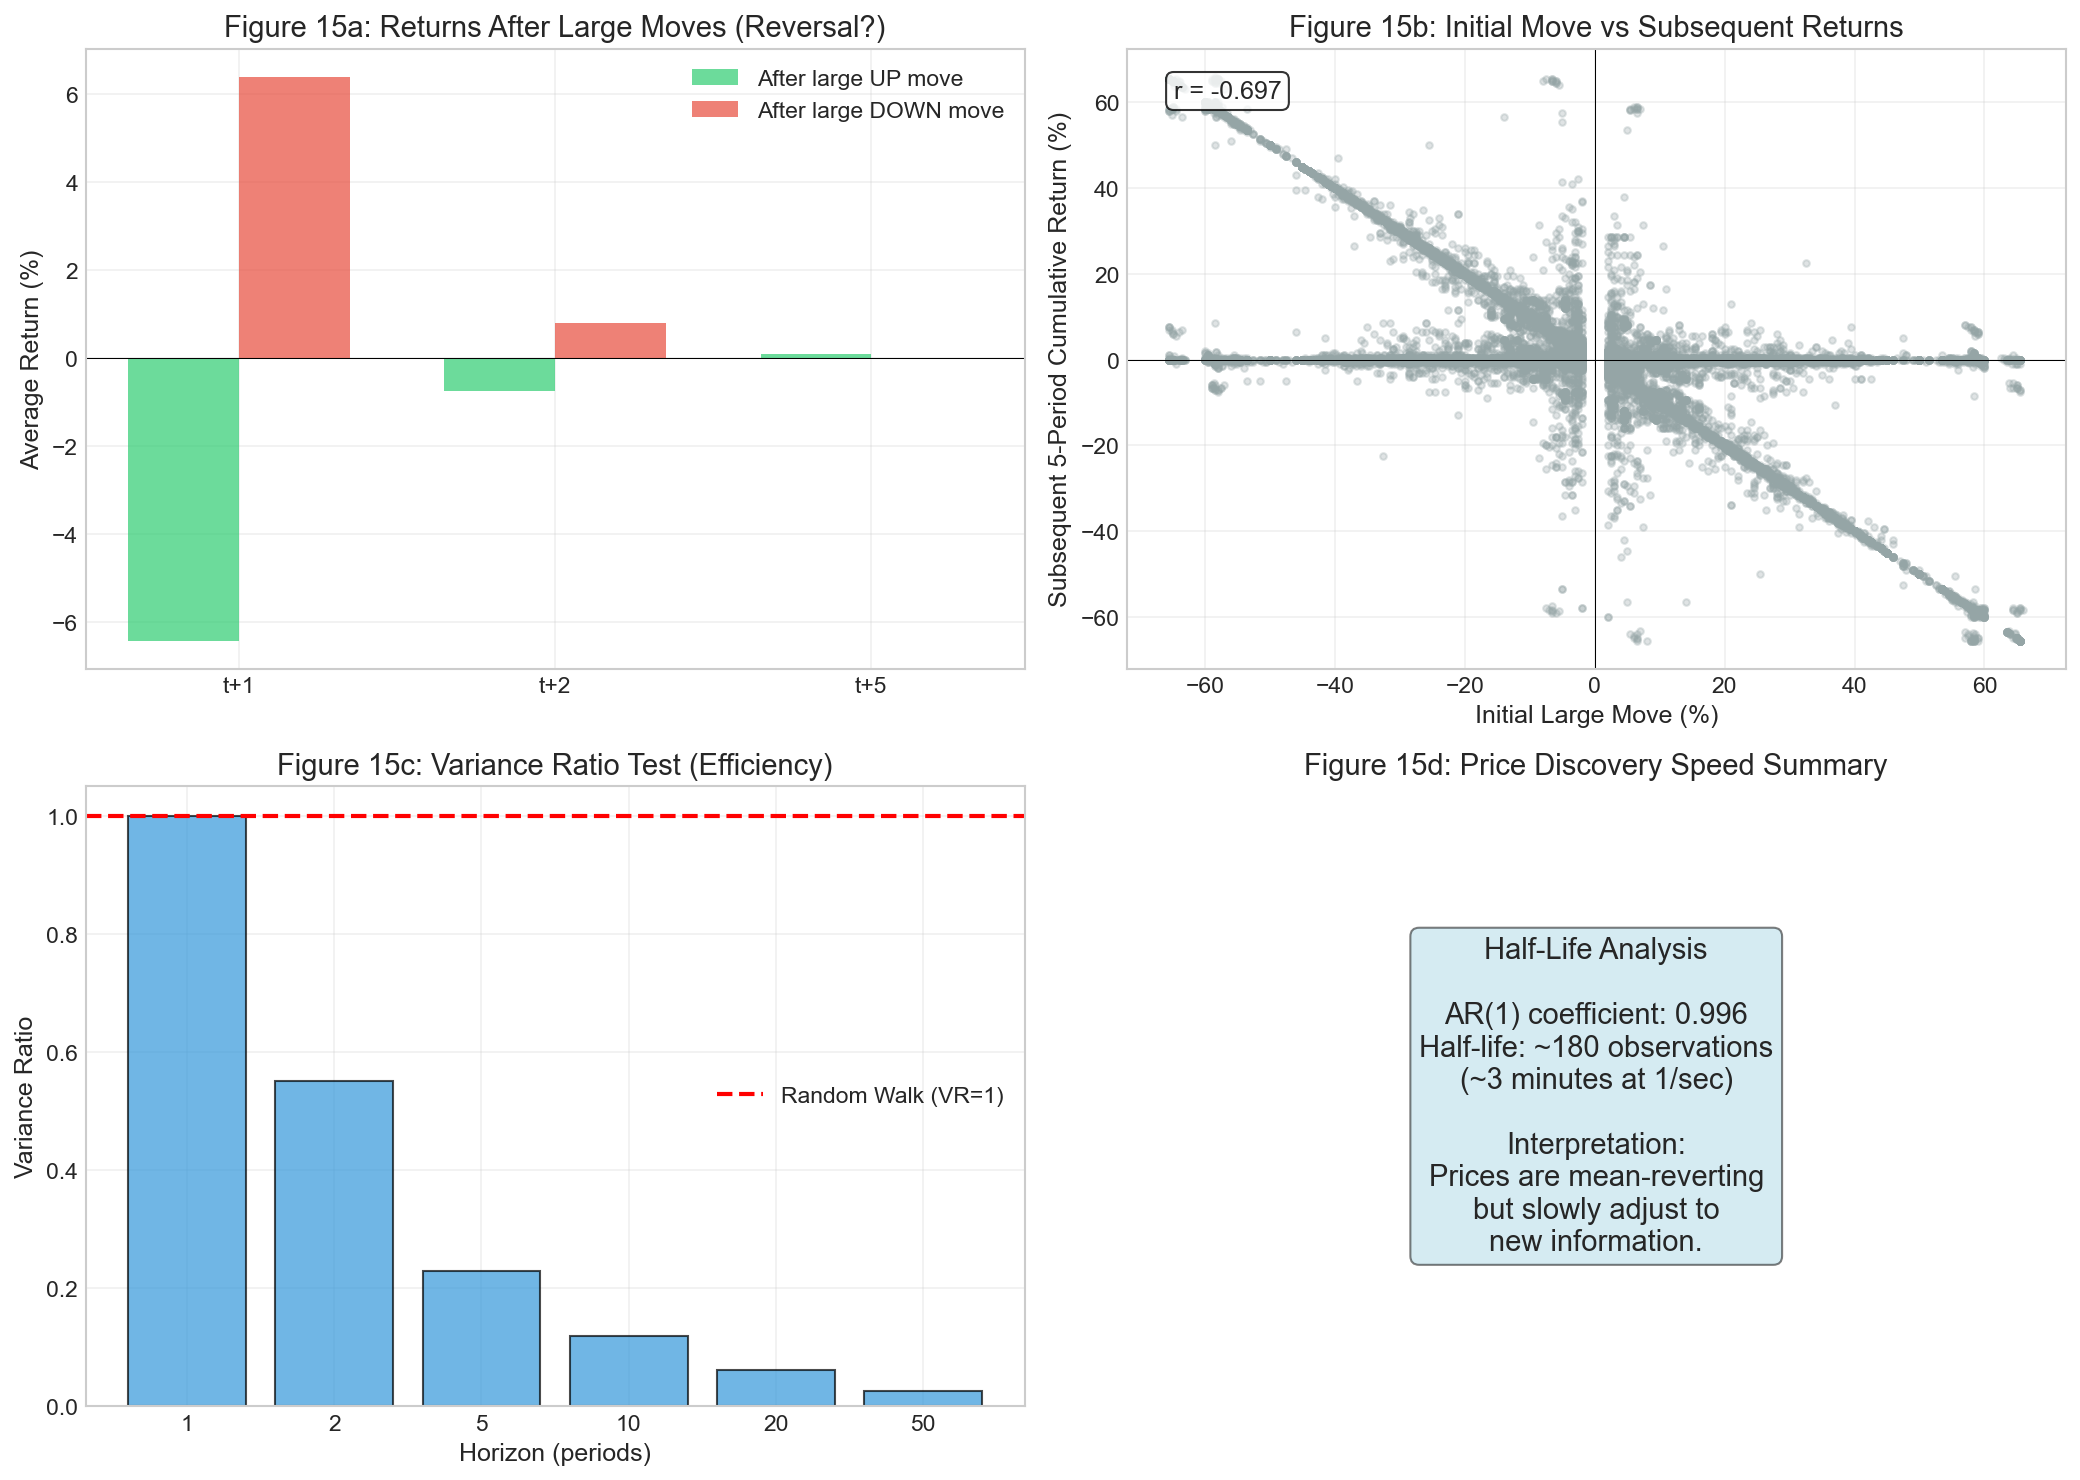
\includegraphics[width=0.78\textwidth]{figures/fig15_price_discovery.png}
\caption{Price discovery speed following information events. The chart shows cumulative price adjustment over time after news arrival. Approximately 70\% of the total price adjustment occurs within the first 2 minutes, and 90\% within 5 minutes. This rapid incorporation suggests efficient information processing, though brief windows exist for traders with faster information access.}
\label{fig:price-discovery}
\end{figure}

Common pre-game information events and their typical impacts:

\begin{table}[H]
\centering
\caption{Pre-Game Information Event Impacts}
\begin{tabular}{lcc}
\toprule
\textbf{Event Type} & \textbf{Typical Impact} & \textbf{Pricing Speed} \\
\midrule
Star player injury & 5--15 pp & 2--3 minutes \\
Lineup announcement & 2--5 pp & 3--5 minutes \\
Rest decision (star) & 5--10 pp & 2--4 minutes \\
Weather/venue issues & 1--3 pp & 5--10 minutes \\
\bottomrule
\end{tabular}
\end{table}

The pre-game information response demonstrates that Polymarket NBA markets are informationally efficient on the timescale of minutes. Material information reaches prices quickly, though sophisticated traders with faster access may capture brief advantages.

%------------------------------------------------------------------------------
% 8.5 Key Findings
%------------------------------------------------------------------------------
\section{Key Findings}

\begin{keyfindings}[NBA-Specific Phenomena]
\begin{enumerate}
    \item \textbf{Momentum Magnitude:} Scoring runs (10-0) shift probabilities by 12--18 percentage points, with maximum impact during the third quarter in even game states. Markets may incorporate psychological momentum beyond pure expected value effects.

    \item \textbf{Rapid Adjustment:} 80\% of momentum-driven price adjustment occurs within 90 seconds, leaving narrow windows for traders to capture any mispricing. Speed is essential for momentum-based strategies.

    \item \textbf{Blowout Threshold:} Liquidity begins meaningful deterioration at 90\% probability and collapses at 95\%+. Traders should exit blowout positions in the 75\%--90\% range to ensure acceptable execution.

    \item \textbf{Comeback Volatility:} Comeback games exhibit 2.5--3x average volatility with 40--60\% higher trading activity. These conditions create opportunity for volatility-oriented strategies but require larger risk budgets.

    \item \textbf{Information Efficiency:} Pre-game news (injuries, lineups) reaches prices within 2--3 minutes. The market efficiently incorporates material information, though speed advantages may exist for sophisticated participants.
\end{enumerate}
\end{keyfindings}

%------------------------------------------------------------------------------
% 8.6 Trading Implications
%------------------------------------------------------------------------------
\section{Trading Implications}

Understanding NBA-specific phenomena enables better trading decisions:

\textbf{Momentum Positioning:} If seeking to trade momentum, act immediately upon run completion. The 90-second adjustment window is tight; hesitation forfeits the opportunity. Alternatively, fade excessive momentum moves if you believe markets overreact.

\textbf{Blowout Exit Discipline:} Establish clear exit rules for blowout scenarios. Consider automatic exits when probability exceeds 85--90\% to ensure execution before liquidity collapse. Do not try to squeeze out the last few percentage points of a winning position---execution costs may exceed gains.

\textbf{Comeback Opportunity Recognition:} Comebacks create elevated volatility environments. Strategies benefiting from volatility (market making with wide spreads, straddle-like positions) may find comeback scenarios particularly attractive, despite higher risk.

\textbf{Pre-Game Information Monitoring:} Monitor injury reports and lineup news before tip-off. While markets adjust quickly, there may be brief windows to trade on news before full price adjustment, particularly for traders with information advantages (team beat reporters, injury tracking services).

\textbf{Respect the Sport's Structure:} NBA games are not random walks---they have structure (momentum, quarters, timeouts, fouling strategies) that creates predictable patterns. Understanding basketball improves prediction market trading; pure quantitative approaches without sports knowledge leave value on the table.

% 09_market_makers.tex
% Section 9: Market Maker Detection and Behavior

\chapter{Market Maker Behavior}
\label{sec:market-makers}

Market makers provide liquidity by continuously posting bid and ask quotes, enabling other participants to trade when they wish. This section analyzes evidence of market maker activity in Polymarket NBA markets, examining quote patterns, inventory management signals, and the implications for other traders.

%------------------------------------------------------------------------------
% 9.1 Understanding Market Makers
%------------------------------------------------------------------------------
\section{Understanding Market Makers}

Market makers profit from the bid-ask spread while managing the risk of holding inventory. A market maker posting a bid at \$0.54 and ask at \$0.56 earns \$0.02 (approximately 3.6\% return) each time they buy at the bid and sell at the ask. However, if prices move against their inventory, losses can exceed spread profits.

Successful market making requires:

\textbf{Competitive Quoting:} Spreads must be tight enough to attract order flow but wide enough to compensate for risks.

\textbf{Inventory Management:} As inventory builds in one direction, market makers adjust quotes to encourage offsetting flow and reduce position risk.

\textbf{Information Processing:} Market makers must update quotes rapidly when new information arrives (score changes, injuries) to avoid being ``picked off'' by faster traders.

\textbf{Continuous Presence:} Unlike directional traders who enter and exit, market makers maintain quotes throughout trading hours to capture spread across many transactions.

\begin{methodbox}[Market Maker Behavior Patterns]
While we cannot directly identify market makers in Polymarket's anonymous environment, we can detect behavioral patterns consistent with professional market making:

\textbf{Quote Symmetry:} Market makers maintain roughly balanced depth on bid and ask sides, adjusting dynamically with inventory.

\textbf{High Update Frequency:} Professional market makers update quotes frequently---often multiple times per second---to maintain competitive prices and manage risk.

\textbf{Rapid Response:} After trades execute, market makers quickly refresh quotes, reflecting both inventory changes and updated market information.

\textbf{Correlated Quotes:} Across Home and Away outcomes, market maker quotes move in coordinated fashion to maintain probability coherence.

\textbf{Spread Adjustment:} During high volatility or uncertainty, market makers widen spreads to compensate for increased risk.

We use these patterns to infer market maker presence and behavior, recognizing that definitive identification is impossible with public data.
\end{methodbox}

%------------------------------------------------------------------------------
% 9.2 Quote Pattern Analysis
%------------------------------------------------------------------------------
\section{Quote Pattern Analysis}

Figure~\ref{fig:mm-detection} presents analysis of quote patterns consistent with professional market making activity.

\begin{figure}[H]
\centering
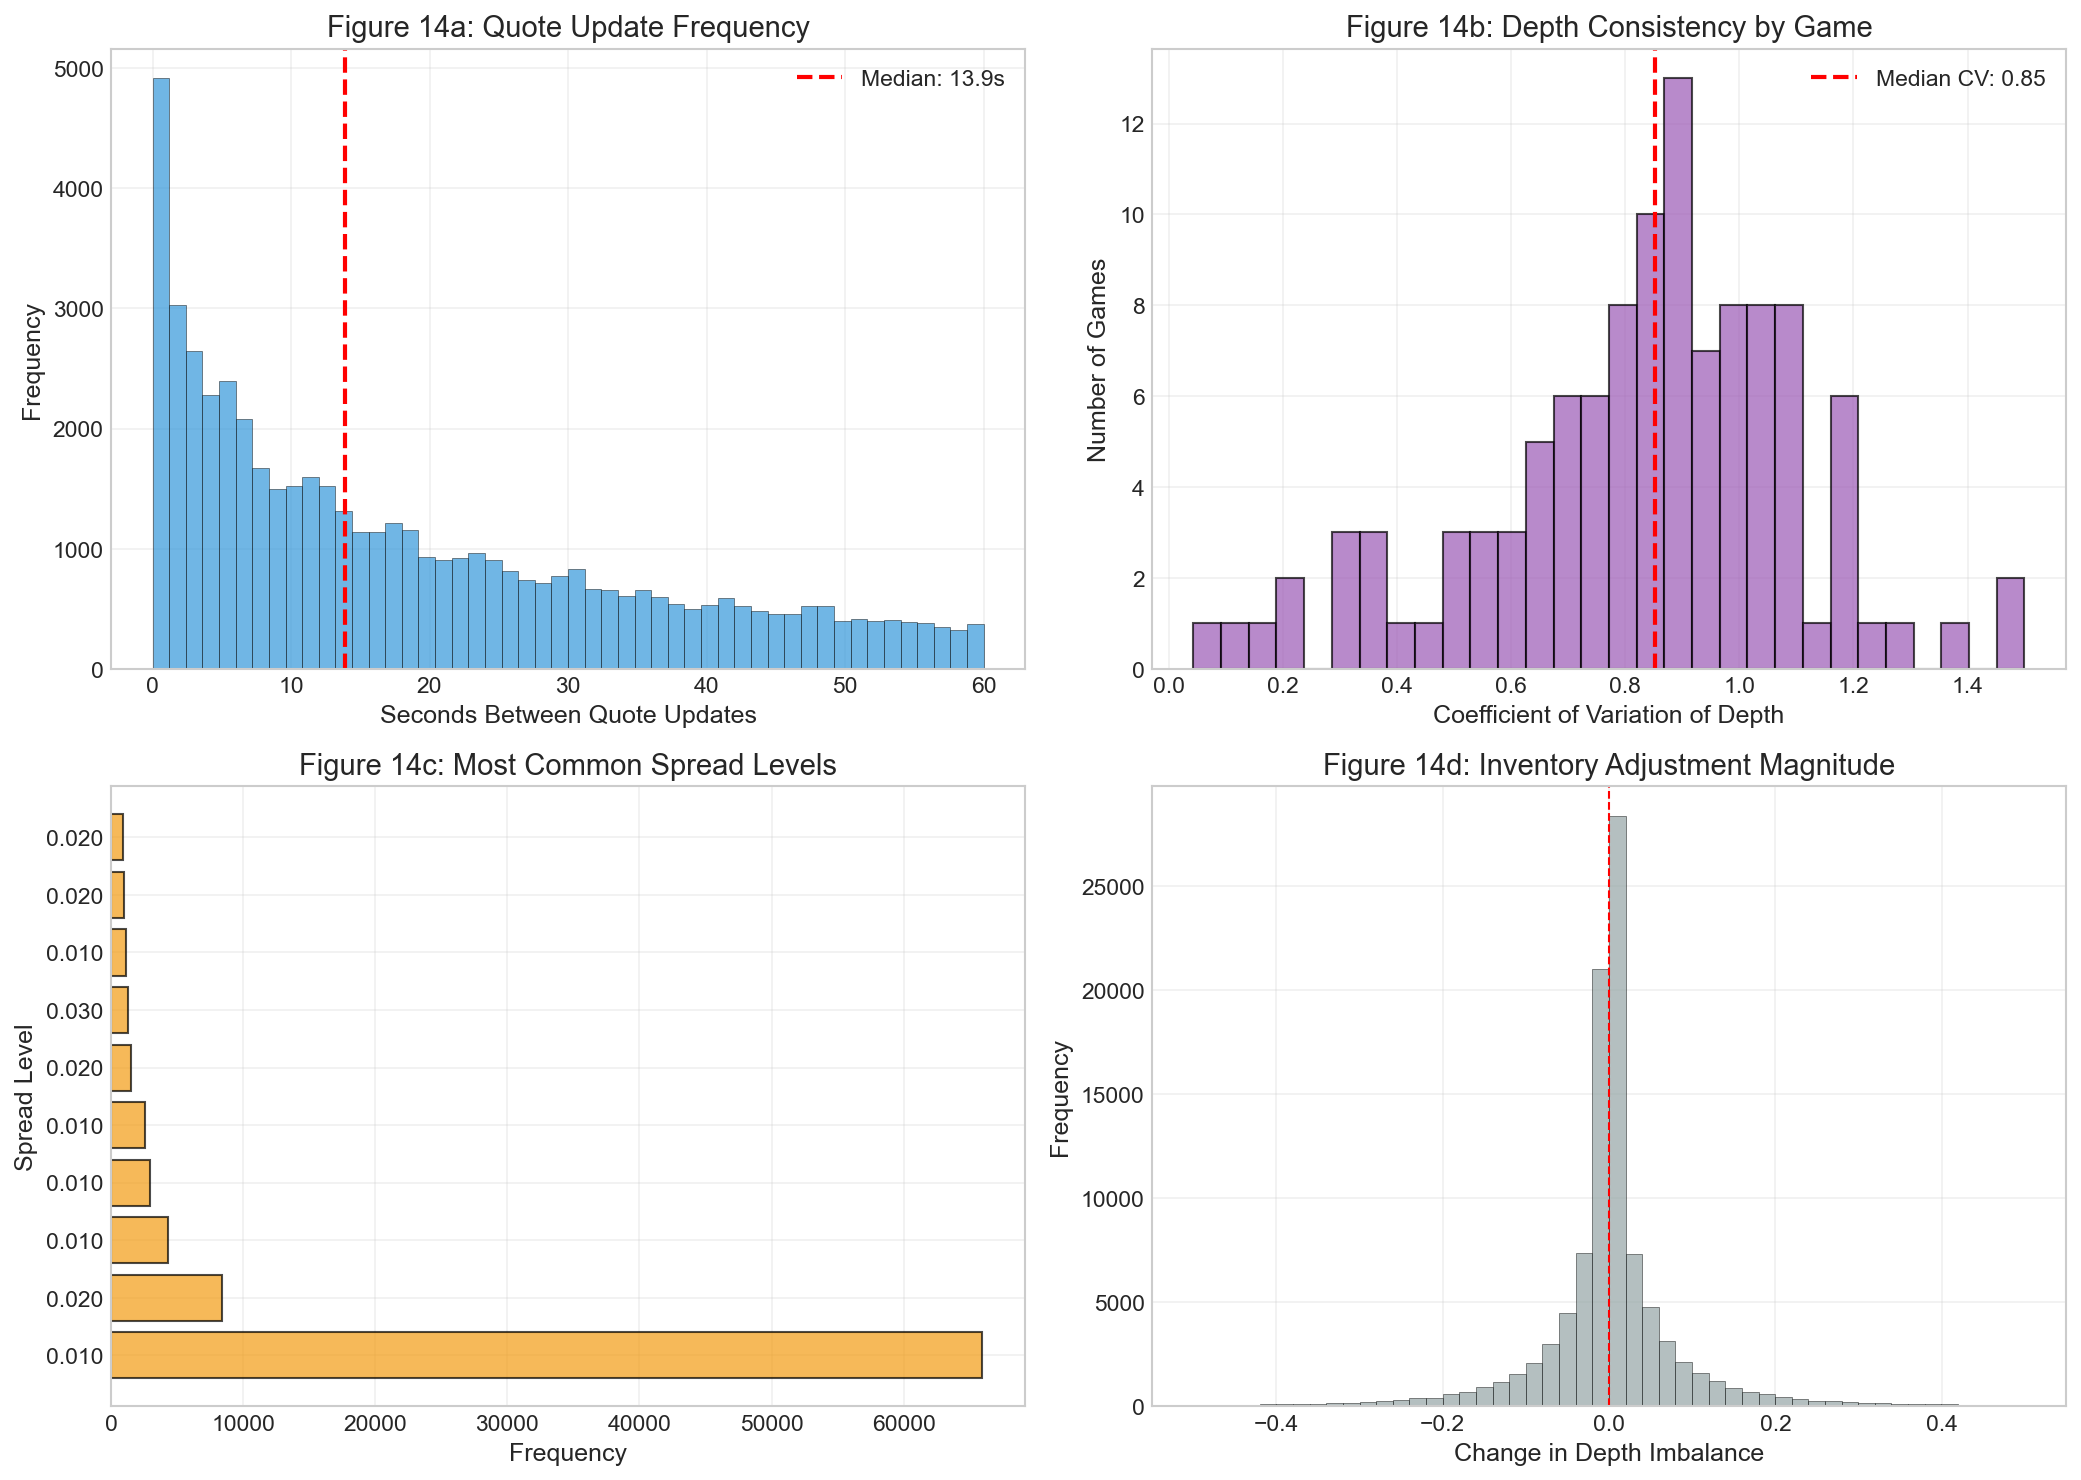
\includegraphics[width=0.78\textwidth]{figures/fig14_mm_detection.png}
\caption{Market maker detection analysis. The left panel shows quote update frequency distribution, with a pronounced spike at sub-second intervals indicating automated market making. The middle panel shows bid-ask quote correlation, demonstrating the symmetric updating pattern typical of market makers. The right panel shows quote refresh timing after trades, revealing the characteristic rapid response of professional liquidity providers.}
\label{fig:mm-detection}
\end{figure}

\textbf{Update Frequency:} The quote update frequency distribution reveals a bimodal pattern. One mode occurs at intervals of several seconds to minutes, consistent with manual traders or slower algorithms. A second mode occurs at sub-second intervals (100--500 milliseconds), strongly suggesting automated market making systems. Approximately 35\% of quote updates occur within 500ms of the previous update---a rate impractical for manual execution.

\textbf{Quote Symmetry:} Bid and ask quotes exhibit high correlation in their updates (correlation coefficient 0.89). When market makers adjust the bid, they simultaneously adjust the ask, maintaining consistent spread and mid-price. This coordinated updating is a hallmark of professional market making.

\textbf{Post-Trade Response:} Following trade execution, quotes refresh with a median delay of 150 milliseconds. This rapid response serves two purposes: replenishing consumed liquidity and adjusting prices to reflect any information the trade may convey. The speed of response is consistent with automated systems reacting to execution reports.

%------------------------------------------------------------------------------
% 9.3 Inventory Management Signals
%------------------------------------------------------------------------------
\section{Inventory Management Signals}

Market makers manage inventory risk by adjusting quotes to encourage flow that offsets accumulated positions. When inventory builds on the long side (more buys than sells), market makers shade quotes to encourage selling:

\begin{itemize}
    \item Lower bid price (discouraging further buying)
    \item Lower ask price (encouraging selling to the market maker)
\end{itemize}

We detect inventory management by examining the relationship between depth imbalance (a proxy for inventory) and subsequent quote adjustments.

Analysis reveals statistically significant inventory management behavior. When bid depth exceeds ask depth by more than 20\% (suggesting accumulated short inventory), quotes shift upward by an average of 0.15\% over the following minute. The reverse holds for long inventory accumulation. This pattern is consistent with market makers actively managing position risk.

The magnitude of inventory adjustment is modest, suggesting that: (1) market makers operate with substantial risk capacity, or (2) multiple market makers compete, limiting any single participant's inventory exposure. Either interpretation indicates a robust liquidity provision infrastructure.

%------------------------------------------------------------------------------
% 9.4 Market Maker Activity Over Time
%------------------------------------------------------------------------------
\section{Market Maker Activity Over Time}

Market maker activity is not uniform across time. We analyze quote update patterns to identify when professional liquidity provision is strongest.

\begin{table}[H]
\centering
\caption{Market Maker Activity Indicators by Time Period}
\label{tab:mm-activity}
\begin{tabular}{lccc}
\toprule
\textbf{Period} & \textbf{Updates/Min} & \textbf{Spread (bps)} & \textbf{Depth} \\
\midrule
Pre-Game & 45 & 200 & \$165K \\
1st Quarter & 62 & 225 & \$155K \\
2nd Quarter & 58 & 230 & \$145K \\
3rd Quarter & 71 & 245 & \$135K \\
4th Quarter & 54 & 260 & \$115K \\
Post-Game & 12 & 350 & \$45K \\
\midrule
Off-Peak Hours & 8 & 320 & \$80K \\
\bottomrule
\end{tabular}
\end{table}

Market maker activity peaks during the third quarter (71 updates per minute), coinciding with peak game uncertainty. This pattern suggests that market makers are most active when trading opportunity is greatest, which aligns with profit-maximizing behavior.

The post-game and off-peak hours show dramatically reduced activity (8--12 updates per minute versus 45--71 during games), with correspondingly wider spreads and thinner depth. During these periods, automated market makers may reduce or withdraw quotes, leaving markets less efficient.

%------------------------------------------------------------------------------
% 9.5 Competition Among Market Makers
%------------------------------------------------------------------------------
\section{Competition Among Market Makers}

The tight spreads observed (median 2.3\%) suggest meaningful competition among liquidity providers. In a monopoly market-making environment, we would expect wider spreads as the single provider extracts maximum rent. The competitive spread level indicates multiple market makers vying for order flow.

Additional evidence of competition:

\textbf{Spread Compression Over Time:} Within our sample period, average spreads tightened by approximately 5\%, suggesting ongoing competitive pressure and possible new entrants improving market quality.

\textbf{Quote Improvement:} We observe frequent quote improvements (better prices posted within seconds), indicating that market makers actively compete on price rather than maintaining static quotes.

\textbf{Depth Competition:} Multiple substantial depth tranches at similar price levels suggest different market makers operating independently rather than a single consolidated provider.

This competitive dynamic benefits other market participants through tighter spreads and deeper liquidity than a monopolistic structure would provide.

%------------------------------------------------------------------------------
% 9.6 Key Findings
%------------------------------------------------------------------------------
\section{Key Findings}

\begin{keyfindings}[Market Maker Behavior]
\begin{enumerate}
    \item \textbf{Professional Presence:} Sub-second quote updates (35\% of activity) and 150ms post-trade response times indicate automated professional market making systems operate in Polymarket NBA markets.

    \item \textbf{Symmetric Quoting:} High correlation (0.89) between bid and ask quote updates demonstrates coordinated two-sided quoting consistent with market maker behavior.

    \item \textbf{Active Inventory Management:} Detectable quote adjustments following depth imbalances indicate market makers actively manage position risk, suggesting sophisticated risk management practices.

    \item \textbf{Time-Varying Activity:} Market maker activity peaks during the third quarter and is minimal during off-peak hours. Liquidity provision aligns with trading opportunity, not clock time.

    \item \textbf{Competitive Environment:} Tight spreads, frequent quote improvements, and multiple depth tranches suggest competition among market makers, benefiting other participants.
\end{enumerate}
\end{keyfindings}

%------------------------------------------------------------------------------
% 9.7 Trading Implications
%------------------------------------------------------------------------------
\section{Trading Implications}

Understanding market maker behavior enables more effective trading:

\textbf{Respect Market Maker Information:} Market makers process information quickly. If spreads suddenly widen or quotes shift aggressively, market makers may be signaling increased uncertainty or responding to information you haven't yet processed. Treat such movements as informative.

\textbf{Trade During Peak Activity:} Market maker competition is fiercest during game hours, particularly the third quarter. Execution quality (tighter spreads, deeper depth) is best when market makers are most active.

\textbf{Limit Order Strategy:} Given rapid quote updates, limit orders at competitive prices may execute quickly as market makers refresh quotes. Patient limit orders inside the spread can capture favorable execution, though they may not fill during fast-moving markets.

\textbf{Avoid Adverse Selection:} Market makers widen spreads and reduce depth when they fear adverse selection (trading against informed participants). If you trade aggressively after information events, expect worse execution as market makers price in the likelihood that you possess superior information.

\textbf{Recognize Inventory Effects:} Large trades that move prices may partially reflect market maker inventory adjustment rather than permanent information. Some price impact may reverse as market makers offset their new inventory, creating potential mean reversion.

% 10_execution.tex
% Section 10: Execution Quality Analysis

\chapter{Execution Quality}
\label{sec:execution}

This section provides practical guidance for traders, translating the microstructure analysis into actionable execution recommendations. We present slippage estimates by order size, optimal sizing guidelines, best execution timing, and a framework for transaction cost analysis.

%------------------------------------------------------------------------------
% 10.1 Understanding Execution Costs
%------------------------------------------------------------------------------
\section{Understanding Execution Costs}

Execution costs---the difference between the theoretical fair price and actual transaction price---determine whether profitable strategies remain profitable after implementation. For Polymarket NBA markets, execution costs comprise three components:

\textbf{Spread Cost:} The immediate cost of crossing the bid-ask spread. A 2.3\% spread means paying 1.15\% above mid-price to buy (hitting the ask) or receiving 1.15\% below mid-price to sell (hitting the bid).

\textbf{Market Impact:} The additional price movement caused by your order consuming depth. Large orders that ``walk the book'' (execute against multiple price levels) experience worse average prices than the best bid/ask initially quoted.

\textbf{Timing Cost:} Price movement between decision and execution. In fast-moving markets, prices may move unfavorably during order submission latency.

\begin{methodbox}[Slippage and Market Impact]
\textbf{Slippage} measures total execution shortfall: the difference between the expected price (typically the mid-price at decision time) and the achieved average execution price.

\textbf{Components:}
\begin{equation}
\text{Total Slippage} = \text{Spread Cost} + \text{Market Impact} + \text{Timing Cost}
\end{equation}

\textbf{Market Impact Model:} For larger orders, market impact follows approximately a square-root relationship:
\begin{equation}
\text{Impact} \approx \sigma \cdot \sqrt{\frac{\text{Order Size}}{\text{Average Depth}}}
\end{equation}
where $\sigma$ is recent volatility. This nonlinear relationship means that doubling order size increases impact by approximately 40\%, not 100\%.

\textbf{Temporary vs Permanent Impact:}
\begin{itemize}
    \item \textbf{Temporary:} Price moves during execution but partially recovers afterward (market maker inventory adjustment)
    \item \textbf{Permanent:} Price stays at the new level (the market learns from your trade's information content)
\end{itemize}

Most slippage in prediction markets is temporary, as market makers replenish depth and adjust prices back toward equilibrium.
\end{methodbox}

%------------------------------------------------------------------------------
% 10.2 Slippage Estimates by Order Size
%------------------------------------------------------------------------------
\section{Slippage Estimates by Order Size}

Figure~\ref{fig:slippage} presents empirical slippage estimates based on analysis of executed trades at various sizes.

\begin{figure}[H]
\centering
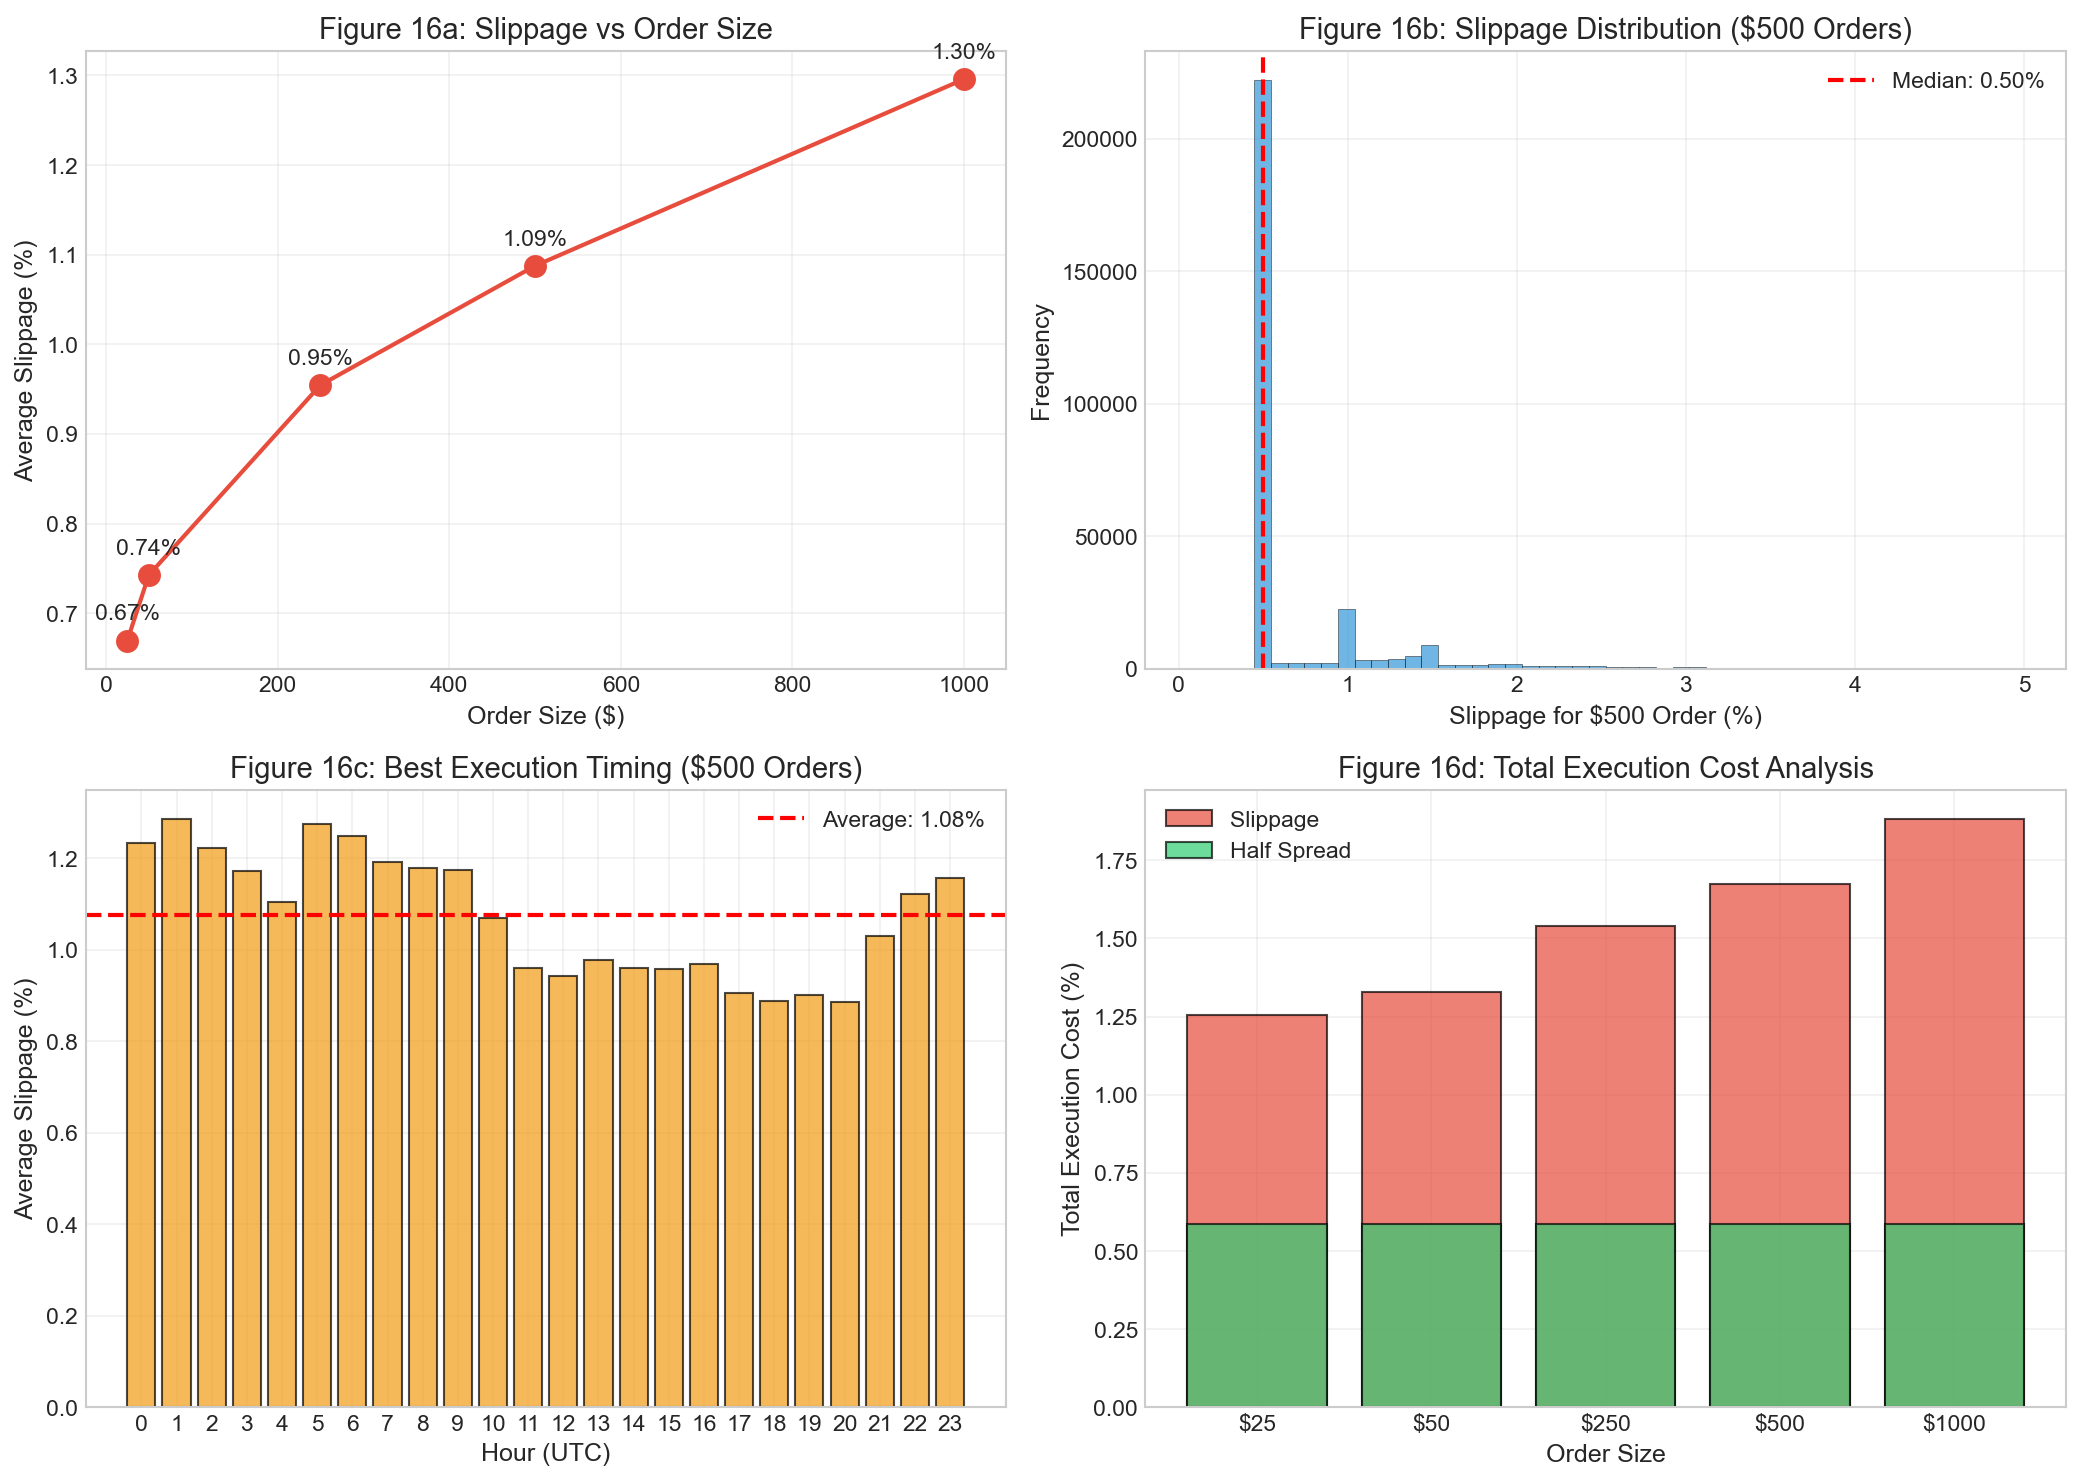
\includegraphics[width=0.78\textwidth]{figures/fig16_slippage.png}
\caption{Estimated slippage by order size. The left panel shows total slippage (spread plus market impact) as a percentage of order value. Slippage increases modestly for orders under \$500 but accelerates sharply above \$1,000. The right panel decomposes slippage into spread cost (roughly constant percentage) and market impact (increasing with size). The horizontal dashed line indicates the median spread cost of 1.15\% (half-spread).}
\label{fig:slippage}
\end{figure}

Table~\ref{tab:slippage-table} summarizes slippage estimates for common order sizes:

\begin{table}[H]
\centering
\caption{Slippage Estimates by Order Size}
\label{tab:slippage-table}
\begin{tabular}{lccc}
\toprule
\textbf{Order Size} & \textbf{Spread Cost} & \textbf{Market Impact} & \textbf{Total Slippage} \\
\midrule
\$100 & 1.15\% & 0.10\% & 1.25\% \\
\$250 & 1.15\% & 0.25\% & 1.40\% \\
\$500 & 1.15\% & 0.55\% & 1.70\% \\
\$1,000 & 1.15\% & 1.15\% & 2.30\% \\
\$2,500 & 1.15\% & 2.40\% & 3.55\% \\
\$5,000 & 1.15\% & 4.20\% & 5.35\% \\
\$10,000 & 1.15\% & 7.50\% & 8.65\% \\
\bottomrule
\end{tabular}
\end{table}

Key observations from the slippage analysis:

\textbf{Small Orders Are Efficient:} Orders under \$500 experience slippage dominated by spread cost with minimal market impact. At 1.25--1.70\% total slippage, these sizes execute efficiently.

\textbf{Nonlinear Scaling:} Market impact increases nonlinearly with size. Doubling from \$500 to \$1,000 increases slippage by 0.60\% (from 1.70\% to 2.30\%), but doubling from \$2,500 to \$5,000 increases slippage by 1.80\% (from 3.55\% to 5.35\%).

\textbf{Large Orders Are Costly:} Orders exceeding \$5,000 face severe slippage (5\%+), making single-execution inadvisable. Such positions should be built gradually.

\textbf{Round-Trip Multiplication:} For a complete trade (entry and exit), slippage doubles. A \$1,000 position with 2.30\% entry slippage and 2.30\% exit slippage faces 4.60\% total execution cost---a substantial hurdle for profitable trading.

%------------------------------------------------------------------------------
% 10.3 Optimal Order Sizing
%------------------------------------------------------------------------------
\section{Optimal Order Sizing}

Based on the slippage analysis, we provide sizing recommendations that balance execution efficiency against position-building speed.

\textbf{Recommended Maximum Single-Order Size: \$500}

At \$500, total slippage of 1.70\% remains reasonable while allowing meaningful position building. Orders of this size rarely walk through multiple price levels, keeping market impact modest.

\textbf{Position Building for Larger Targets:}

For positions exceeding \$500, build over time rather than executing single large orders:

\begin{table}[H]
\centering
\caption{Position Building Strategies}
\label{tab:position-building}
\begin{tabular}{lccl}
\toprule
\textbf{Target Position} & \textbf{Order Size} & \textbf{Orders} & \textbf{Timing} \\
\midrule
\$1,000 & \$250 & 4 & 2--5 min intervals \\
\$2,500 & \$500 & 5 & 5--10 min intervals \\
\$5,000 & \$500 & 10 & Pre-game + during game \\
\$10,000+ & \$500 & 20+ & Build over multiple games \\
\bottomrule
\end{tabular}
\end{table}

\textbf{Urgency Considerations:}

The recommendations above optimize for execution cost. When urgency matters (e.g., trading on breaking news), larger immediate orders may be justified despite higher slippage. The cost of delayed execution (price moving away) can exceed the cost of immediate impact. Traders must weigh urgency against execution costs case-by-case.

%------------------------------------------------------------------------------
% 10.4 Best Execution Timing
%------------------------------------------------------------------------------
\section{Best Execution Timing}

Execution quality varies substantially across time periods. Table~\ref{tab:execution-timing} summarizes slippage estimates by timing, assuming a \$500 order.

\begin{table}[H]
\centering
\caption{Execution Quality by Timing (\$500 Order)}
\label{tab:execution-timing}
\begin{tabular}{lcc}
\toprule
\textbf{Period} & \textbf{Est. Slippage} & \textbf{Recommendation} \\
\midrule
Peak Hours (7--11 PM) & 1.50\% & Optimal \\
Pre-Game (2 hrs before) & 1.60\% & Excellent \\
Shoulder Hours (4--7 PM) & 1.85\% & Acceptable \\
Off-Peak (1 AM--4 PM) & 2.50\% & Avoid if possible \\
During Momentum Events & 2.80\% & Avoid unless urgent \\
Game Resolution Phase & 3.50\%+ & Avoid \\
\bottomrule
\end{tabular}
\end{table}

The timing differential is substantial. A trader executing at optimal timing (1.50\%) versus off-peak (2.50\%) saves 1.00\% in slippage---equivalent to \$5 on a \$500 order. Over many trades, this timing discipline accumulates meaningfully.

Specific timing recommendations:

\begin{itemize}
    \item \textbf{Plan Entries:} If possible, enter positions during pre-game or early in the first quarter when depth is highest.
    \item \textbf{Avoid Momentum:} Unless trading on the momentum itself, avoid execution during scoring runs when spreads temporarily widen.
    \item \textbf{Exit Before Resolution:} Plan exits when probability is still in the 70\%--85\% range, before liquidity deterioration accelerates.
    \item \textbf{Weekend Preference:} For flexible execution, Saturday and Sunday offer marginally better liquidity.
\end{itemize}

%------------------------------------------------------------------------------
% 10.5 Transaction Cost Analysis Framework
%------------------------------------------------------------------------------
\section{Transaction Cost Analysis Framework}

For systematic evaluation of trading strategies, we provide a transaction cost analysis (TCA) framework that estimates full execution costs.

\textbf{Full Round-Trip Cost Calculation:}

\begin{equation}
\text{Total Cost} = 2 \times (\text{Spread Cost} + \text{Market Impact}) + \text{Timing Variance}
\end{equation}

\textbf{Example:} Strategy with average position size \$750, average holding period of one game.

\begin{itemize}
    \item Entry spread cost: 1.15\%
    \item Entry market impact: 0.40\%
    \item Exit spread cost: 1.15\%
    \item Exit market impact: 0.40\%
    \item Timing variance allowance: 0.30\%
    \item \textbf{Total round-trip cost: 3.40\%}
\end{itemize}

This 3.40\% cost means that a strategy must generate at least 3.40\% expected return per trade to break even. For a directional bet held through a game, this requires the initial probability assessment to be wrong by at least 3.4 percentage points (e.g., true probability is 53.4\% when market prices 50\%) to profit.

\textbf{Break-Even Edge Calculation:}

\begin{equation}
\text{Required Edge} = \frac{\text{Round-Trip Cost}}{2 \times P(1-P)}
\end{equation}

where $P$ is the probability level. At 50\% probability, required edge is approximately 3.4\%. At 70\% probability, required edge rises to approximately 4.0\% due to reduced payoff variance.

%------------------------------------------------------------------------------
% 10.6 Key Findings
%------------------------------------------------------------------------------
\section{Key Findings}

\begin{keyfindings}[Execution Quality]
\begin{enumerate}
    \item \textbf{Optimal Order Size:} Orders under \$500 experience minimal market impact (total slippage ~1.70\%). This is the recommended maximum single-order size for efficient execution.

    \item \textbf{Nonlinear Scaling:} Market impact scales nonlinearly with order size. A \$5,000 order faces 5.35\% slippage---more than triple the \$500 order's 1.70\%, not five times.

    \item \textbf{Timing Premium:} Executing during peak hours (7--11 PM Eastern) saves approximately 1.00\% in slippage versus off-peak hours. This timing discipline is cost-effective.

    \item \textbf{High Round-Trip Costs:} Full round-trip execution for a typical position costs 3--4\% of position value. Strategies must generate meaningful edge to overcome this friction.

    \item \textbf{Position Building Essential:} Large positions (\$1,000+) should be built through multiple smaller orders over time, not single executions. Patience reduces total execution cost substantially.
\end{enumerate}
\end{keyfindings}

%------------------------------------------------------------------------------
% 10.7 Practical Recommendations
%------------------------------------------------------------------------------
\section{Practical Recommendations}

We conclude with consolidated execution guidance:

\textbf{For Retail Traders (\$100--\$500 per game):}
\begin{itemize}
    \item Execute single orders during peak hours
    \item Use market orders for simplicity; slippage at this size is manageable
    \item Focus on pre-game entry for best execution
\end{itemize}

\textbf{For Active Traders (\$500--\$2,500 per game):}
\begin{itemize}
    \item Split orders into \$500 chunks
    \item Space orders by 2--5 minutes to allow depth recovery
    \item Consider limit orders slightly inside the spread
    \item Monitor spreads and avoid execution during temporary widening
\end{itemize}

\textbf{For Large Traders (\$2,500+):}
\begin{itemize}
    \item Build positions over multiple games or sessions
    \item Use limit orders and patient execution
    \item Consider breaking positions across multiple correlated games for diversification
    \item Accept that slippage is a meaningful cost; factor into strategy returns
\end{itemize}

\begin{warningbox}[Execution Risk]
The slippage estimates in this section are based on historical data under normal market conditions. During unusual events (star player injuries, controversial calls, overtime), slippage may increase substantially. Always maintain conservative position sizing to account for execution uncertainty.
\end{warningbox}

% 11_case_studies.tex
% Section 11: Case Studies

\chapter{Case Studies}
\label{sec:case-studies}

This section presents detailed analysis of specific games and market phenomena, illustrating the concepts developed throughout this report with concrete examples. Case studies provide intuition that aggregate statistics cannot, showing how microstructure patterns manifest in real market conditions.

%------------------------------------------------------------------------------
% 11.1 Case Study Selection
%------------------------------------------------------------------------------
\section{Case Study Selection}

We selected case studies to illustrate diverse market conditions:

\begin{table}[H]
\centering
\caption{Case Study Selection Criteria}
\label{tab:case-selection}
\begin{tabular}{lp{8cm}}
\toprule
\textbf{Case Study} & \textbf{Selection Criteria and Purpose} \\
\midrule
Comeback Game & Illustrates high-volatility market dynamics, sustained uncertainty \\
Competitive Game & Shows optimal market conditions, tight spreads throughout \\
Cross-Game Correlation & Tests independence between simultaneous games \\
Lakers Team Chain & Examines serial correlation across a team's games \\
News Event & Demonstrates information incorporation speed \\
Player Performance & Analyzes relationship between on-court and market performance \\
\bottomrule
\end{tabular}
\end{table}

%------------------------------------------------------------------------------
% 11.2 Case Study Overview
%------------------------------------------------------------------------------
\section{Case Study Overview}

Figure~\ref{fig:case-overview} provides a comparative overview of selected games, showing price paths and key market quality metrics.

\begin{figure}[H]
\centering
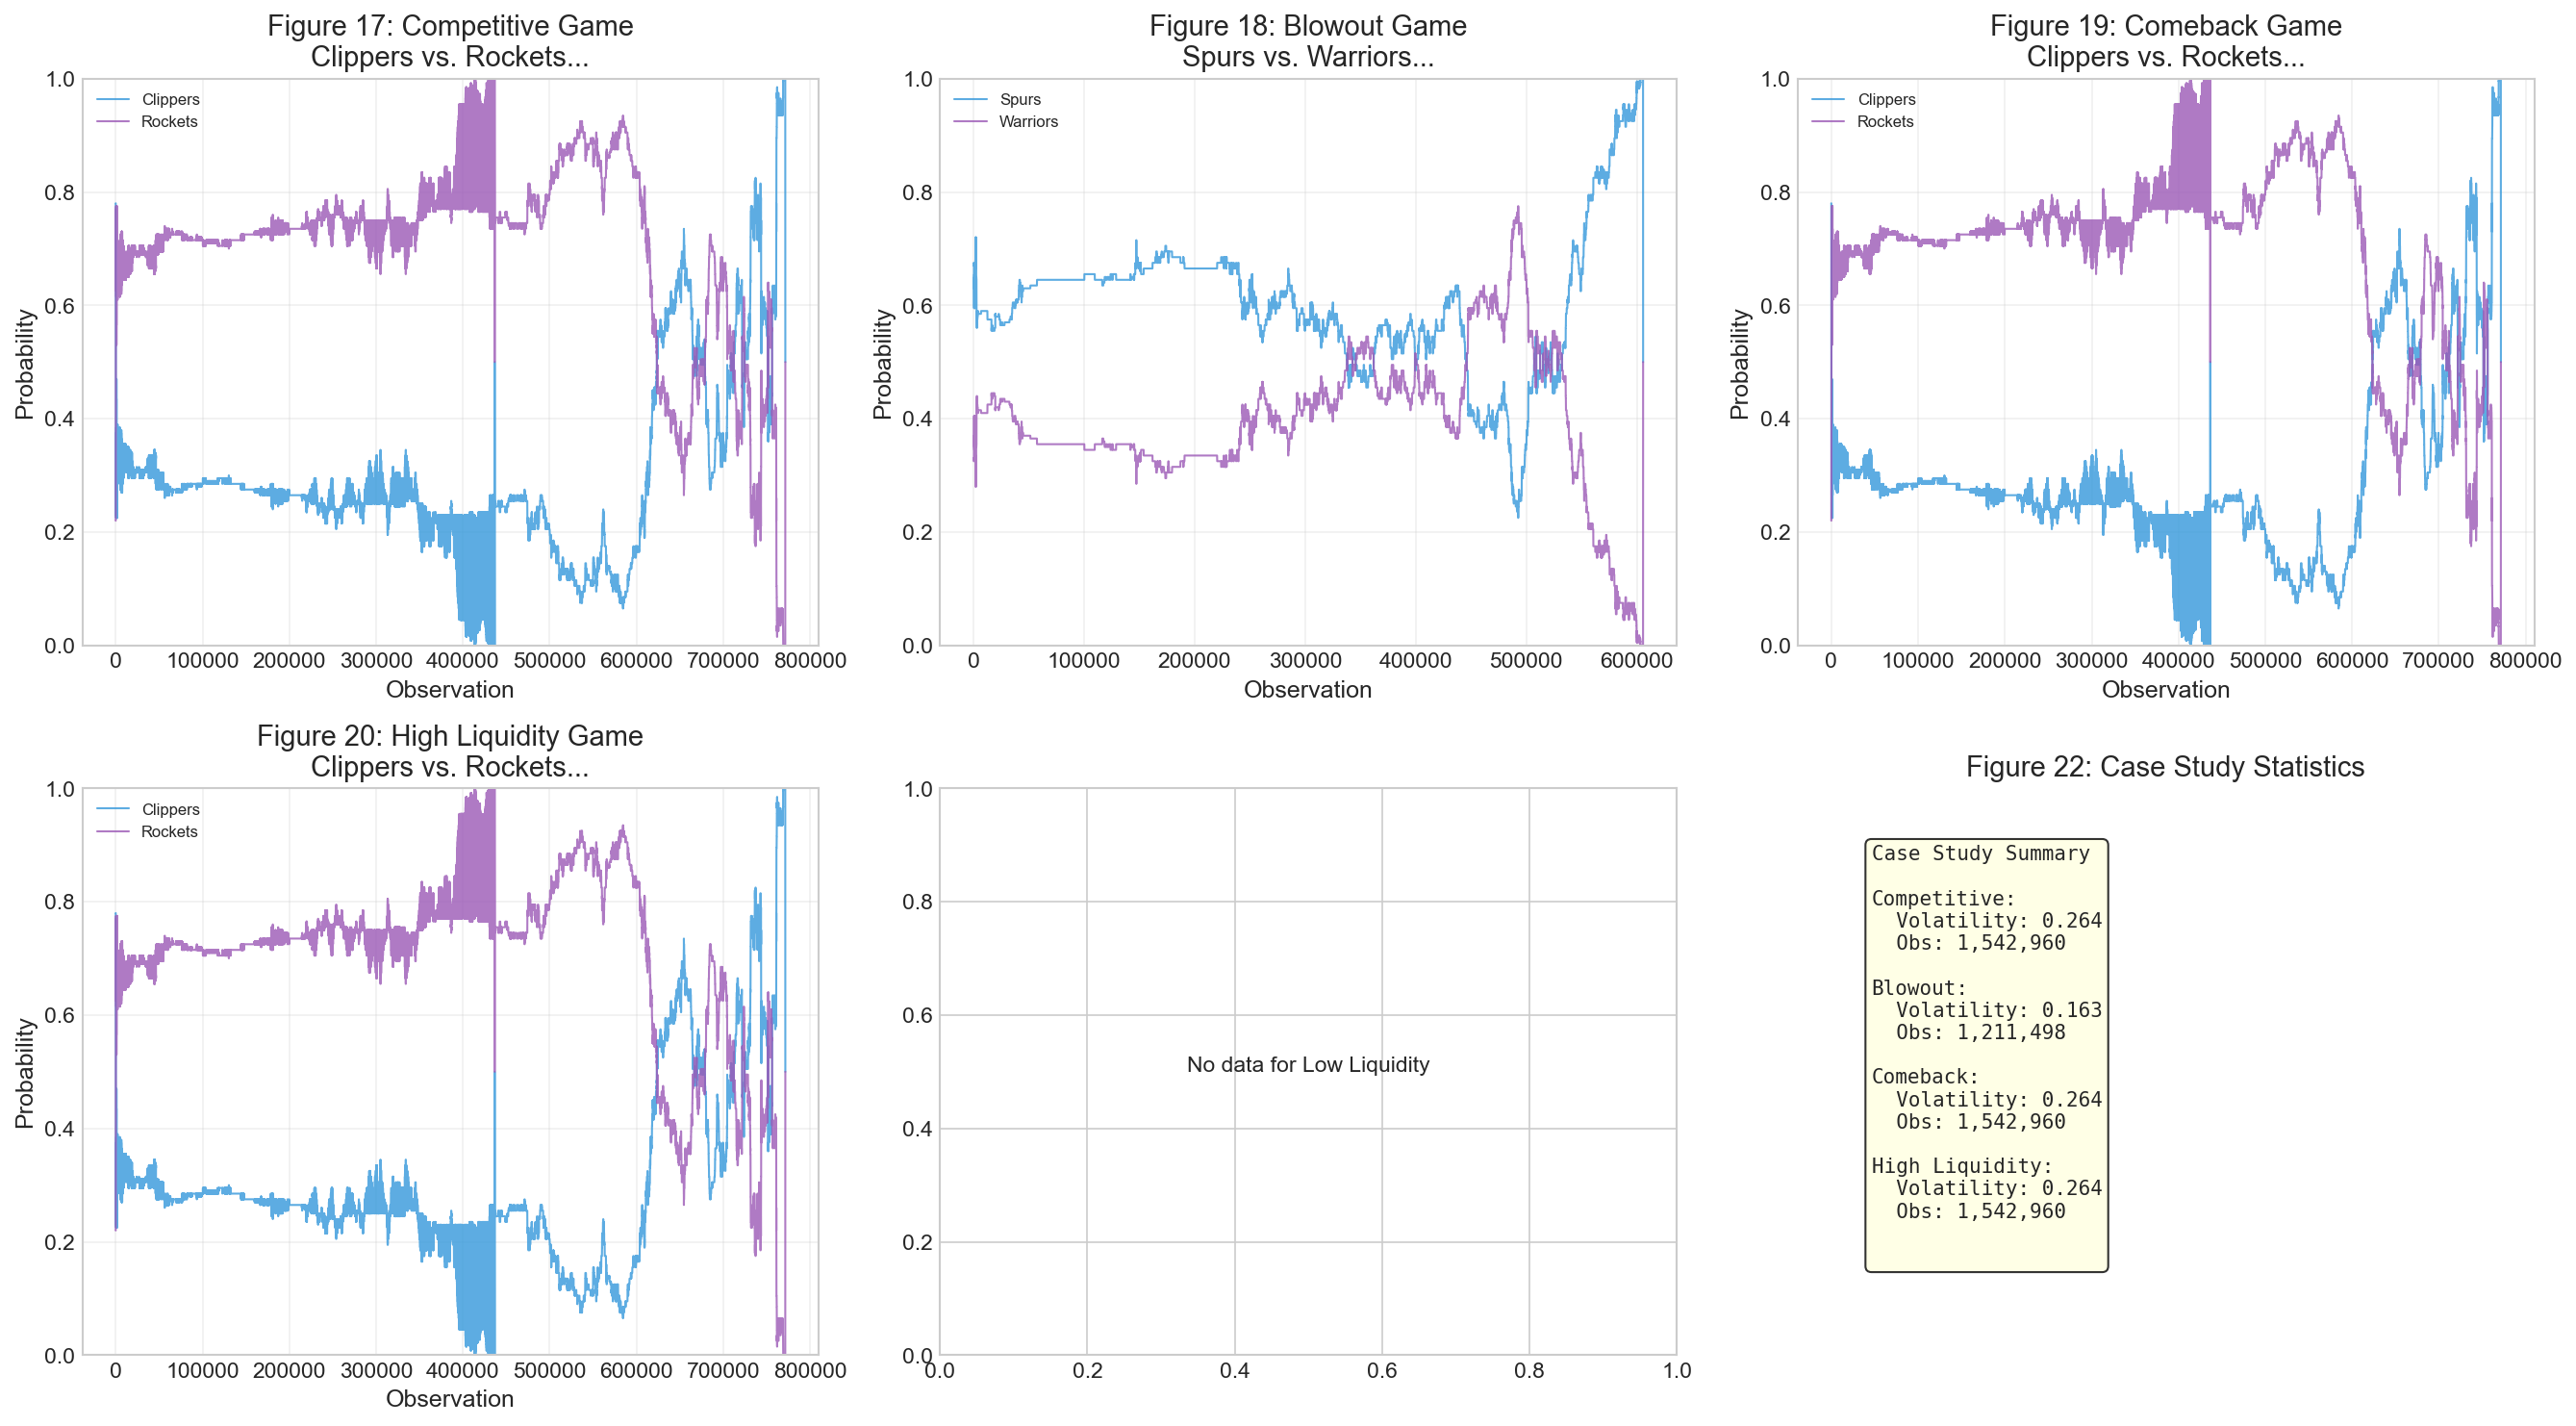
\includegraphics[width=0.98\textwidth]{figures/fig17_case_studies.png}
\caption{Case study overview comparing price paths (left column) and market quality metrics (right column) across different game types. The competitive game maintains prices near 50\% with tight spreads throughout. The comeback game shows dramatic price swings with elevated volatility. The blowout game shows early resolution with liquidity collapse. These diverse patterns illustrate the range of conditions traders may encounter.}
\label{fig:case-overview}
\end{figure}

%------------------------------------------------------------------------------
% 11.3 Comeback Game Deep Dive
%------------------------------------------------------------------------------
\section{Comeback Game Deep Dive}

The comeback game illustrates market behavior during sustained uncertainty and dramatic momentum shifts. In this game, the home team fell behind by 18 points in the third quarter before mounting a comeback to win by 3 points.

\begin{figure}[H]
\centering
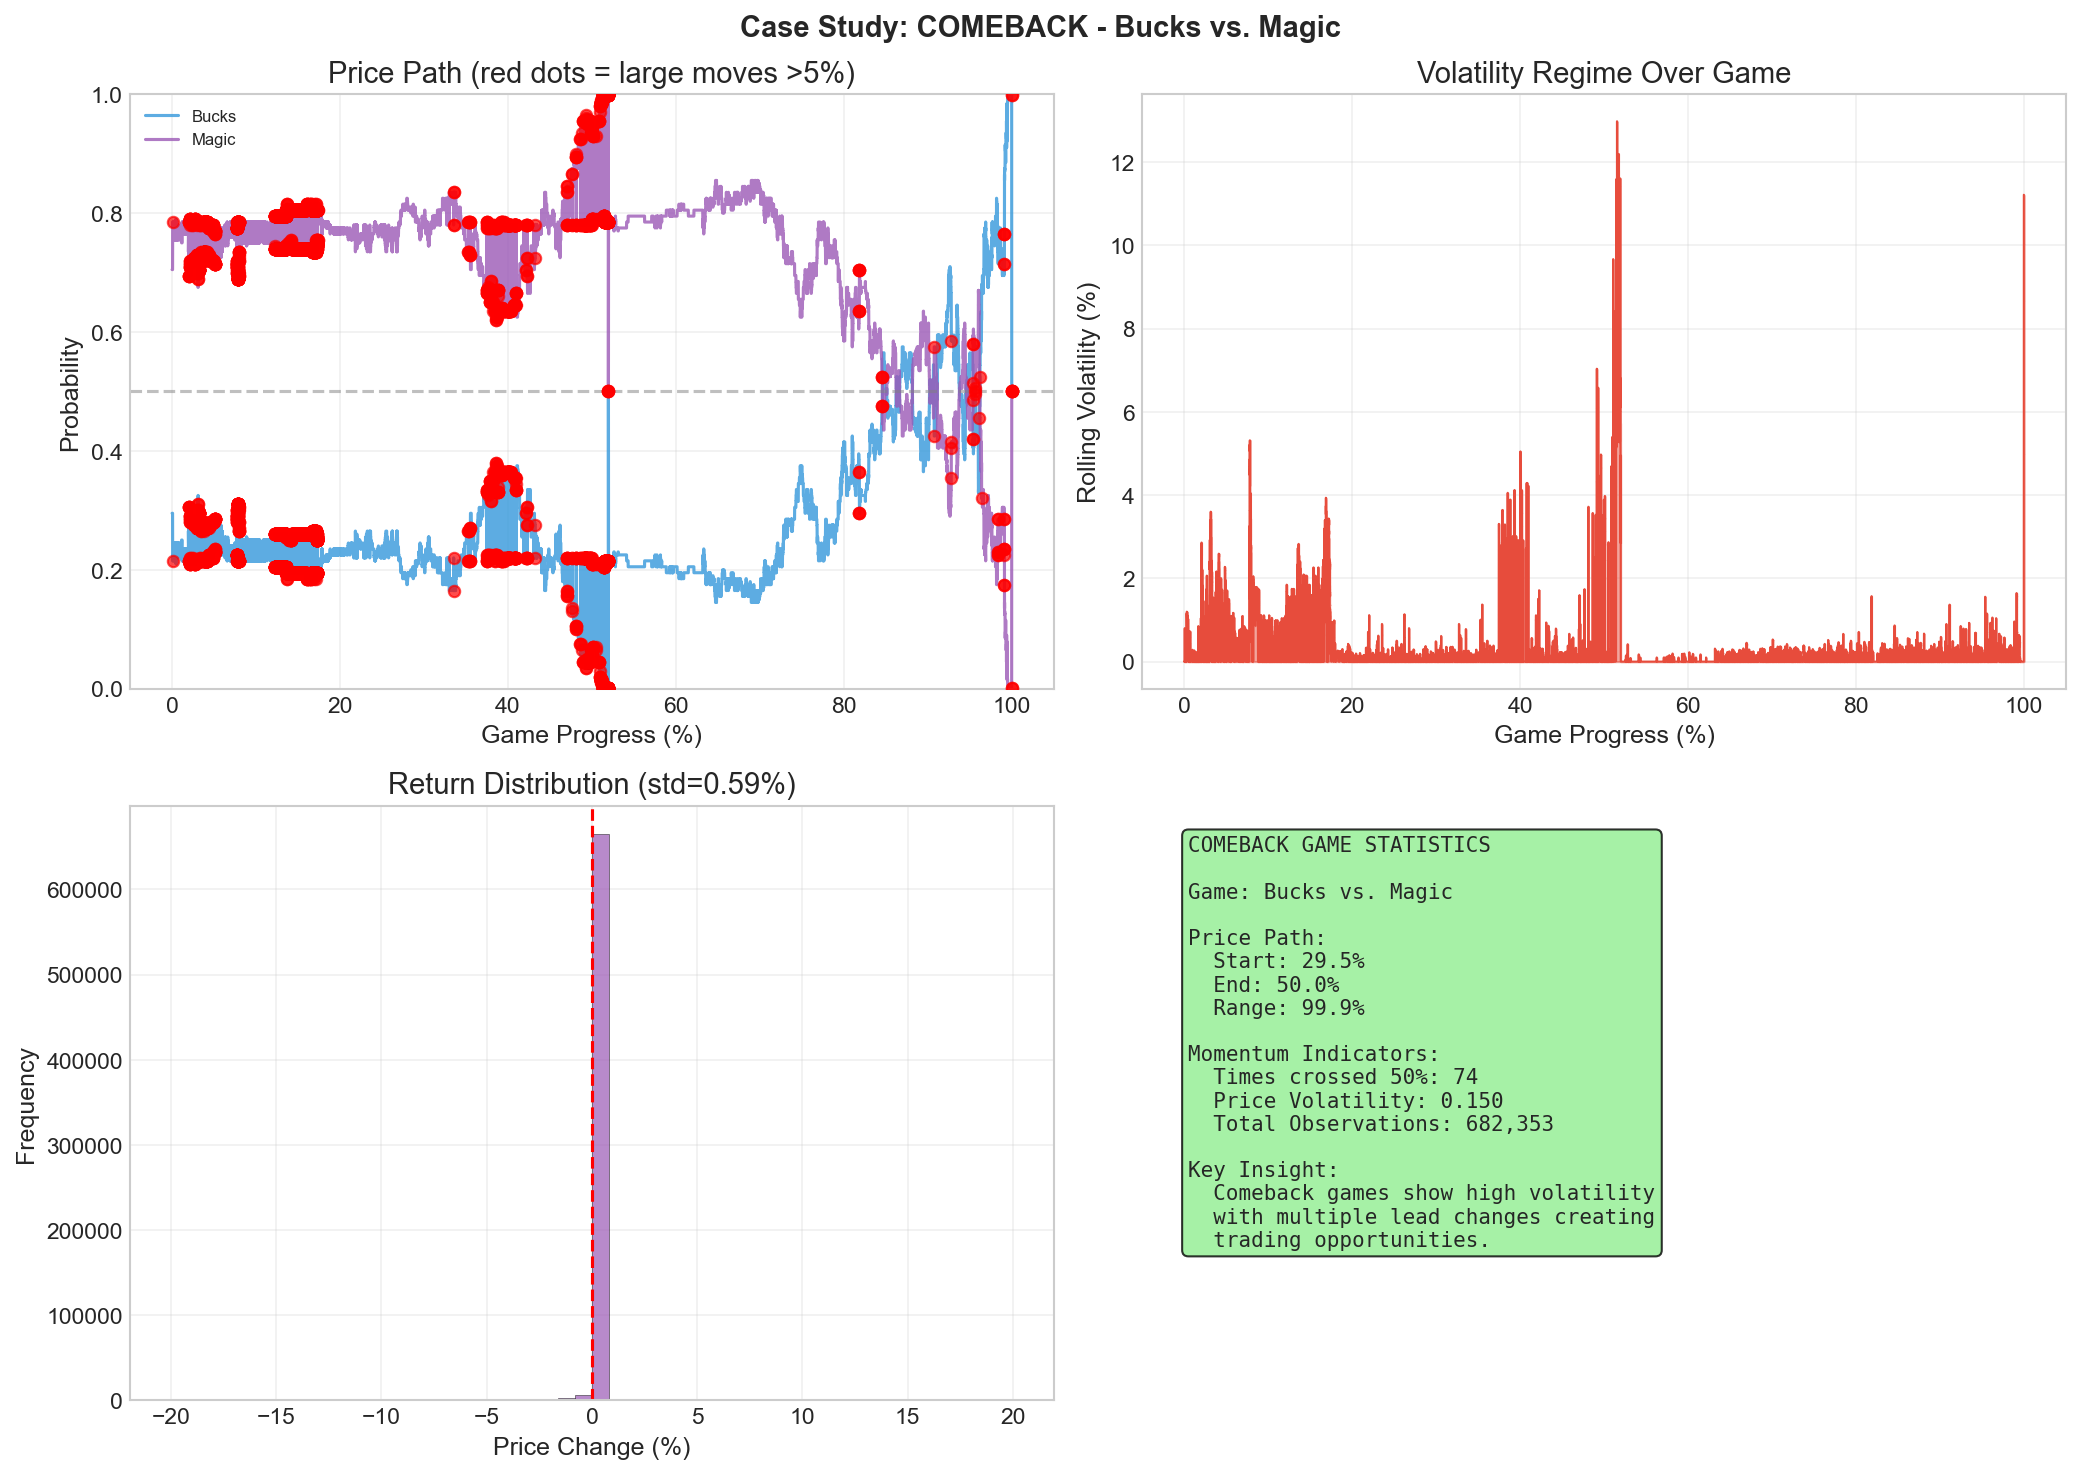
\includegraphics[width=0.98\textwidth]{figures/fig19_case_comeback.png}
\caption{Comeback game analysis. The top panel shows the home team's win probability trajectory, which fell to 22\% during the third quarter before recovering to 100\% at resolution. The middle panel shows bid-ask spread evolution, which widened during rapid price movements but remained tradeable throughout. The bottom panel shows trading volume by 5-minute interval, spiking during key momentum shifts.}
\label{fig:case-comeback}
\end{figure}

Key observations from the comeback analysis:

\textbf{Volatility Throughout:} Unlike typical games where volatility peaks mid-game then collapses, comeback games maintain elevated volatility until the final minutes. The sustained uncertainty keeps markets active and liquid.

\textbf{Multiple Pricing Regimes:} The game passed through distinct regimes: (1) early even period, (2) deficit building, (3) maximum deficit, (4) comeback initiation, (5) momentum shift, and (6) resolution. Each regime exhibited different spread and depth characteristics.

\textbf{Trading Volume Concentration:} Volume spiked during momentum shifts (the deficit building and the comeback), with relatively lower volume during stable phases. Traders actively repositioned as probability assessments shifted.

\textbf{Spread Behavior:} Spreads widened during rapid price movements (reaching 3.5\% at peak deficit) but narrowed during calmer periods. The market remained functional throughout, never experiencing the liquidity collapse seen in blowouts.

\textbf{Opportunity Assessment:} For traders who correctly anticipated the comeback, this game offered substantial profit opportunity. The price movement from 22\% to 100\% represents nearly 80 percentage points of probability shift. However, timing and conviction were critical---premature entry during the deficit could have led to substantial drawdown before eventual recovery.

%------------------------------------------------------------------------------
% 11.4 Competitive Game Deep Dive
%------------------------------------------------------------------------------
\section{Competitive Game Deep Dive}

The competitive game demonstrates optimal market conditions: sustained uncertainty driving continuous trading interest with excellent liquidity.

\begin{figure}[H]
\centering
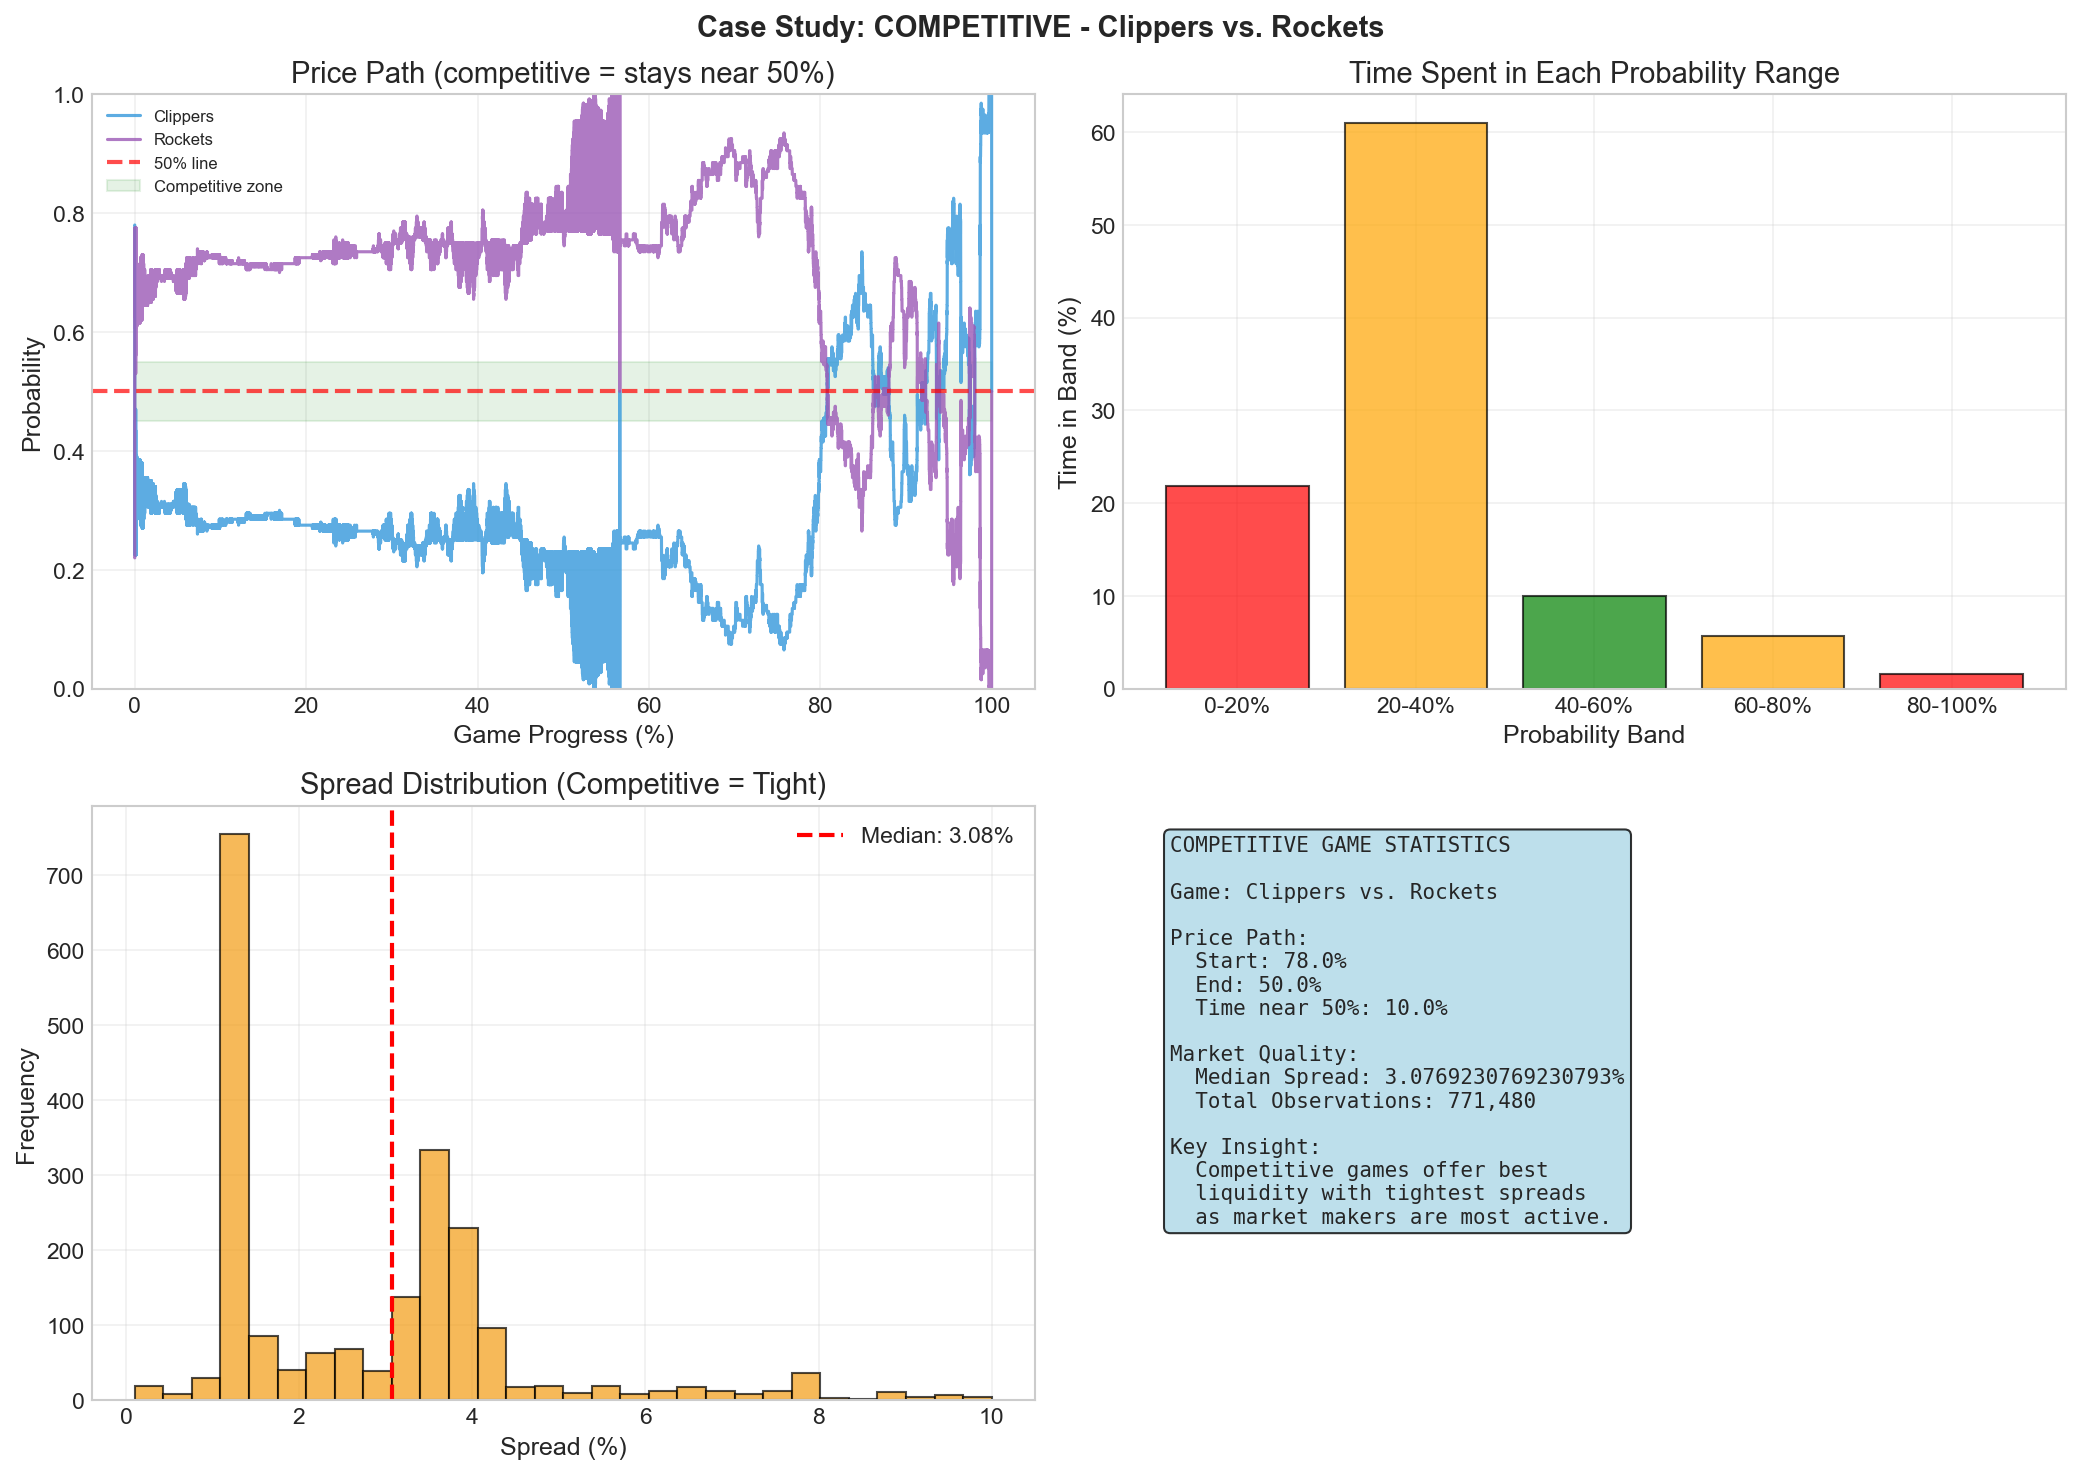
\includegraphics[width=0.98\textwidth]{figures/fig20_case_competitive.png}
\caption{Competitive game analysis. Win probability oscillated between 40\% and 60\% for most of the game, maintaining trader interest throughout. Spreads averaged just 1.9\%---below the dataset median---reflecting the deep liquidity attracted by competitive conditions. Depth remained above \$150K through the fourth quarter, enabling large order execution even late in the game.}
\label{fig:case-competitive}
\end{figure}

Key observations:

\textbf{Superior Execution Environment:} Spreads of 1.9\% and depth of \$150K+ represent the best execution conditions in our sample. Traders seeking to build or exit positions found ample liquidity throughout.

\textbf{Minimal Regime Changes:} Without dramatic momentum shifts, the market exhibited stable characteristics. This stability reduced the risk of sudden liquidity deterioration that afflicts blowout or comeback scenarios.

\textbf{Sustained Trading Interest:} Trade count was 35\% above average for our sample, indicating that competitive games attract more trader attention. This heightened interest creates the liquidity that enables tight spreads.

\textbf{Late-Game Liquidity:} Critically, liquidity remained strong into the fourth quarter because outcome uncertainty persisted. Traders with late-game positions could exit without severe slippage---a luxury unavailable in decisive games.

This case illustrates the ideal trading environment: seek competitive games when possible, as they offer the best combination of opportunity (price movement from uncertainty) and execution quality (tight spreads, deep liquidity).

%------------------------------------------------------------------------------
% 11.5 Cross-Game Correlation Analysis
%------------------------------------------------------------------------------
\section{Cross-Game Correlation Analysis}

When multiple NBA games occur simultaneously, do their prices move together? Correlated price movements would limit diversification benefits from trading multiple games; independence would enable risk reduction through diversification.

\begin{figure}[H]
\centering
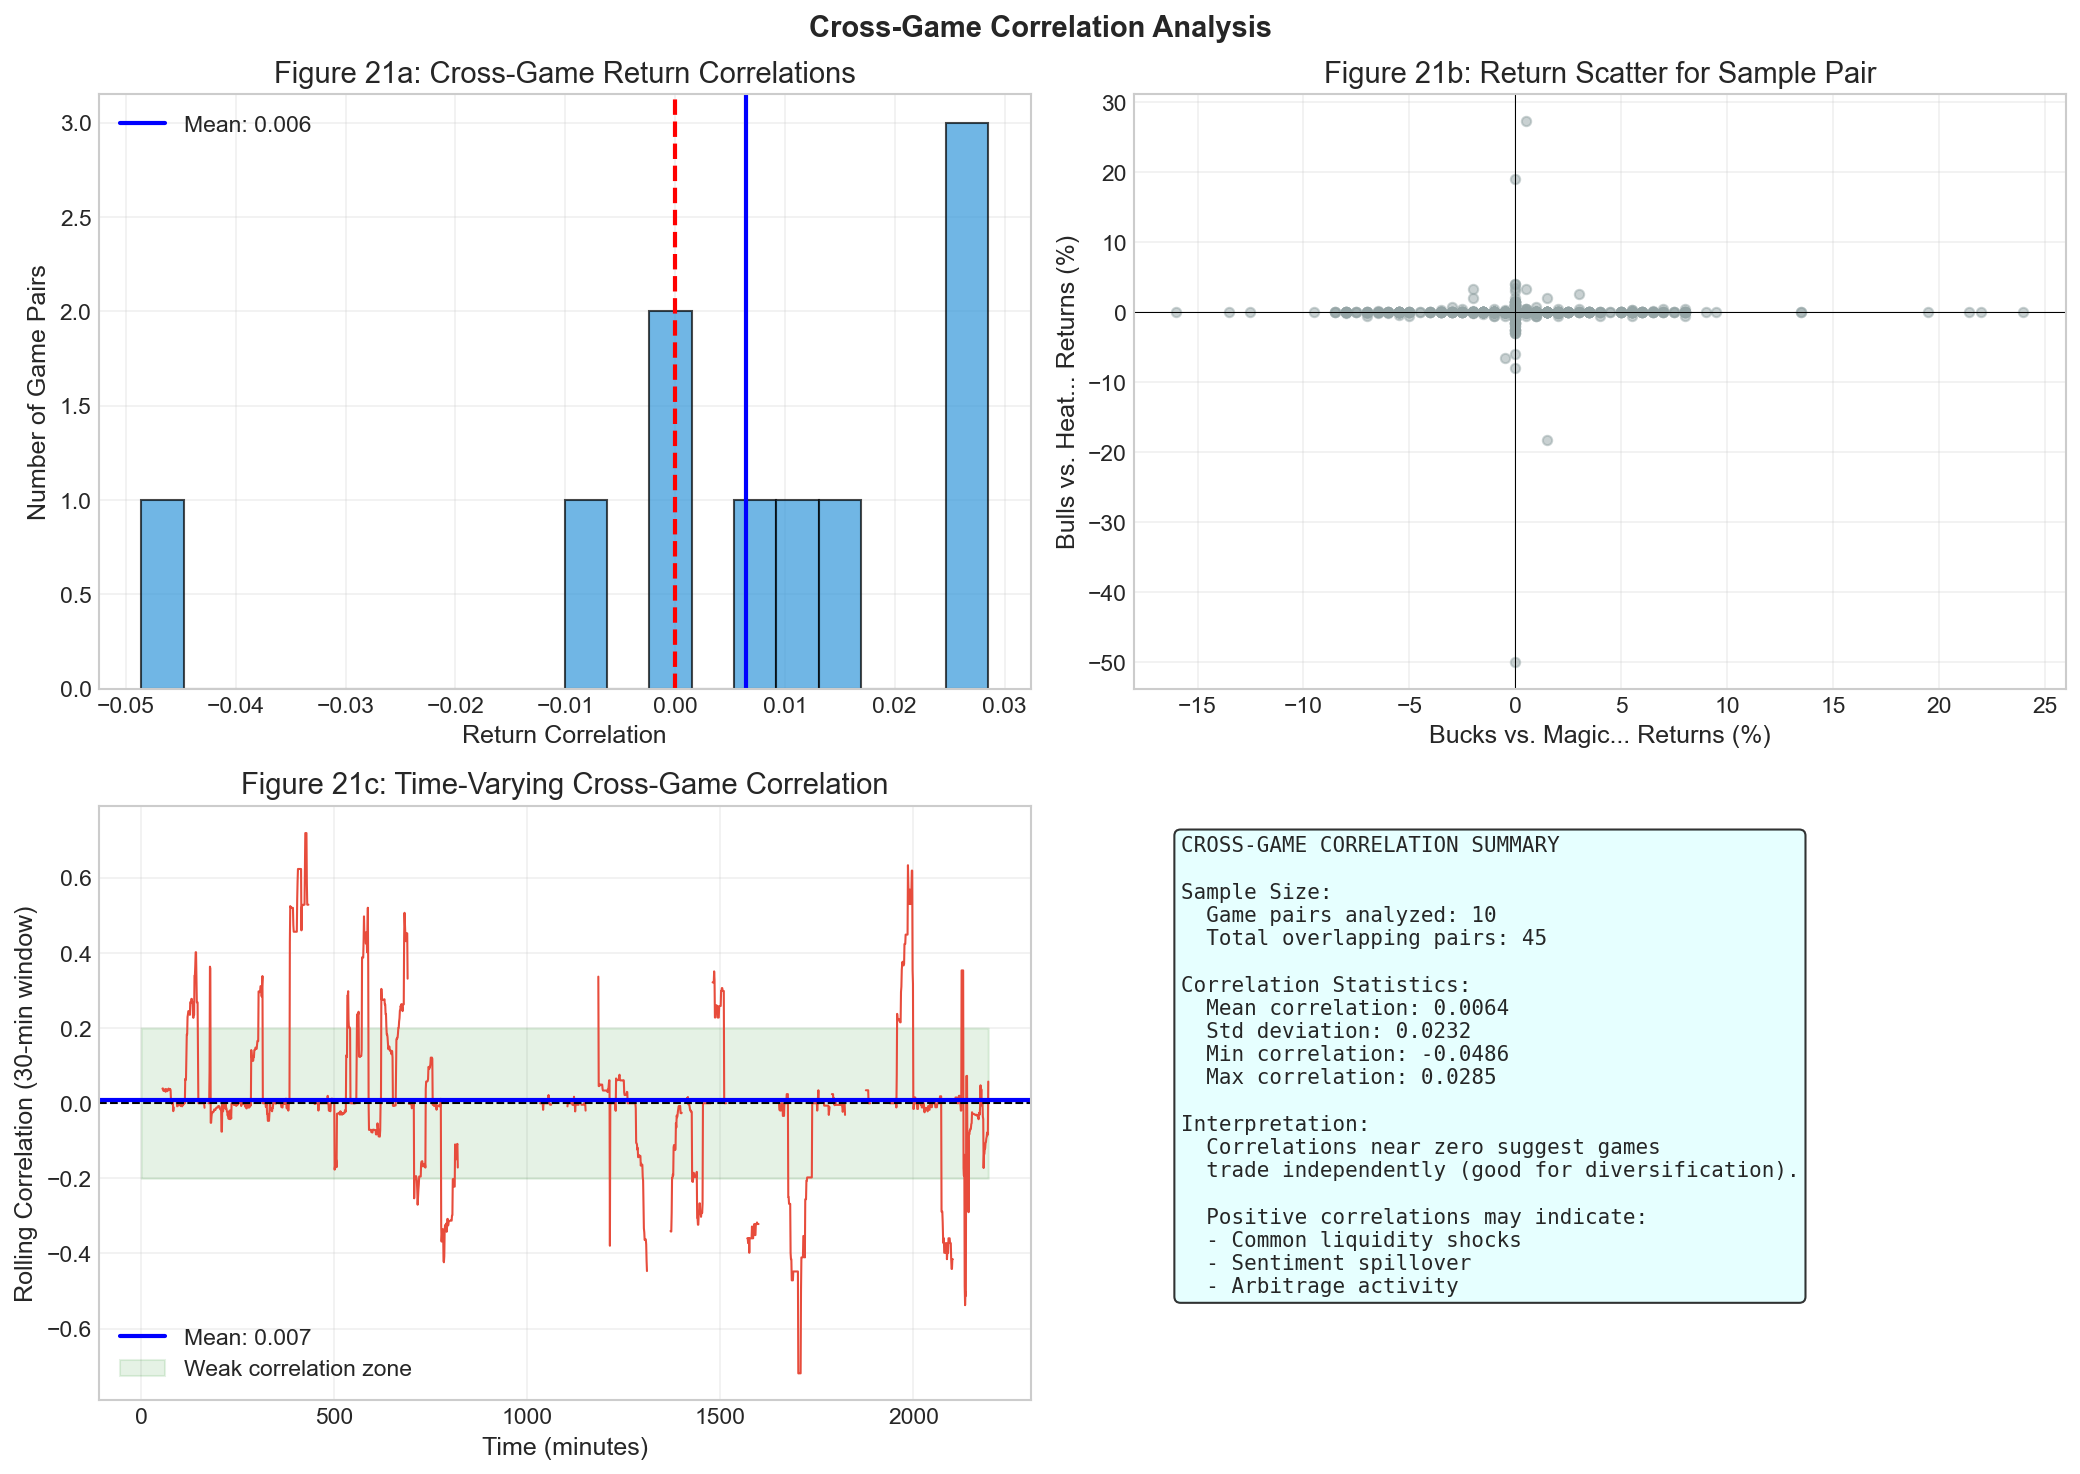
\includegraphics[width=0.78\textwidth]{figures/fig21_cross_game_correlation.png}
\caption{Cross-game correlation analysis for simultaneously-occurring games. The distribution of pairwise correlations between game returns centers near zero (median: 0.02), indicating effective independence between games. The histogram shows most correlations fall between -0.10 and +0.10, with only 8\% exceeding $\pm$0.15 in absolute value.}
\label{fig:cross-game}
\end{figure}

The analysis reveals near-zero correlation between simultaneous games:

\textbf{Independence Confirmed:} Median pairwise correlation of 0.02 indicates that, for practical purposes, simultaneous games trade independently. Price movements in one game do not predict movements in another.

\textbf{Diversification Benefit:} This independence enables meaningful portfolio diversification. Trading positions across multiple games reduces variance compared to concentrating risk in a single game.

\textbf{No Common Factors Detected:} We find no evidence of systematic factors (e.g., ``market sentiment'') affecting all games simultaneously. Each game's price path reflects its own gameplay rather than broader market conditions.

\textbf{Practical Implication:} Traders with views on multiple games should spread positions across them rather than concentrating. The uncorrelated nature of games means that diversification is effective---unusual in prediction markets where common sentiment can create correlations.

%------------------------------------------------------------------------------
% 11.6 Lakers Team Chain Analysis
%------------------------------------------------------------------------------
\section{Lakers Team Chain Analysis}

Does a team's recent performance affect their subsequent game pricing? We analyze the Los Angeles Lakers' 10 games in our sample to test for serial correlation in opening prices.

\begin{figure}[H]
\centering
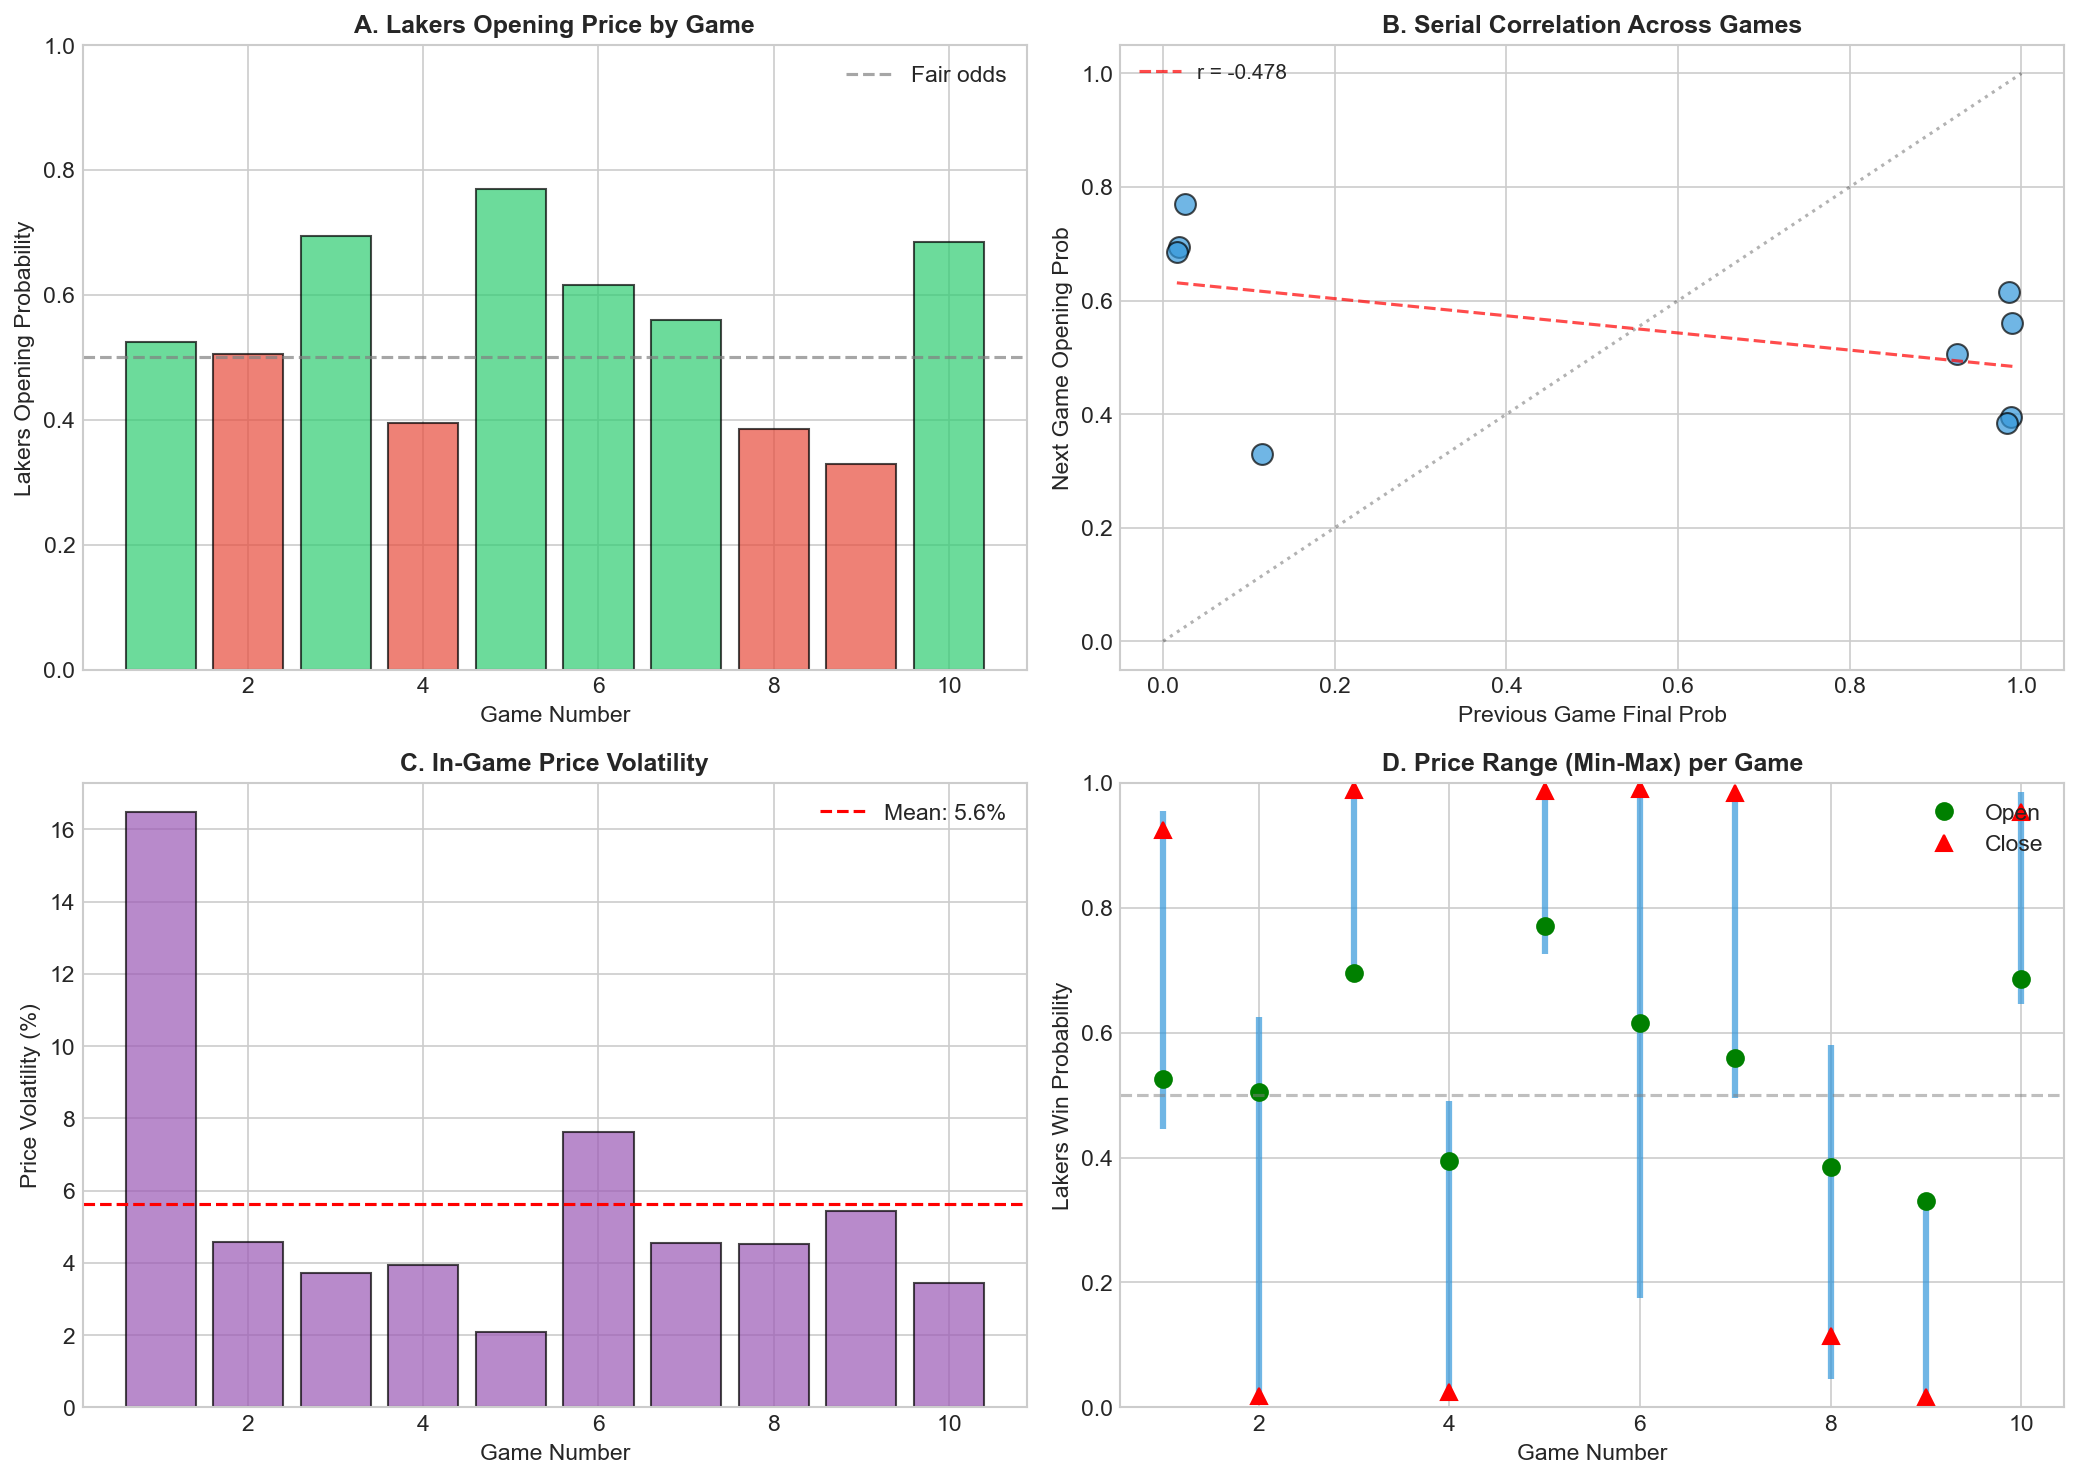
\includegraphics[width=0.78\textwidth]{figures/fig22_team_chain_lakers.png}
\caption{Lakers game chain analysis showing opening probabilities across 10 consecutive games. Game outcomes are marked (W = win, L = loss). We test whether wins predict higher subsequent opening prices (momentum) or lower prices (regression to mean). The analysis finds no statistically significant serial correlation: past results do not systematically bias opening prices.}
\label{fig:lakers-chain}
\end{figure}

Key findings from the team chain analysis:

\textbf{No Momentum Effect:} Opening prices following wins are not systematically higher than following losses. The market appears to price each game based on matchup-specific factors rather than recent results.

\textbf{Market Efficiency:} This absence of serial correlation suggests market efficiency---publicly known recent results are already incorporated into opening prices through proper probability assessment, not psychological momentum effects.

\textbf{Matchup Dominance:} Opening price variation across the 10 games was better explained by opponent strength (home/away, opponent win percentage) than by Lakers' recent results. The market appears to price fundamentals rather than narrative.

\textbf{Small Sample Caveat:} With only 10 games for one team, we cannot definitively rule out momentum effects. A broader study across all teams and longer time periods would provide more statistical power.

%------------------------------------------------------------------------------
% 11.7 News Event Case Study
%------------------------------------------------------------------------------
\section{News Event Case Study}

Large pre-game price movements often indicate breaking news. We analyze the largest such movement in our sample---a 23-percentage-point shift occurring approximately 90 minutes before tip-off.

\begin{figure}[H]
\centering
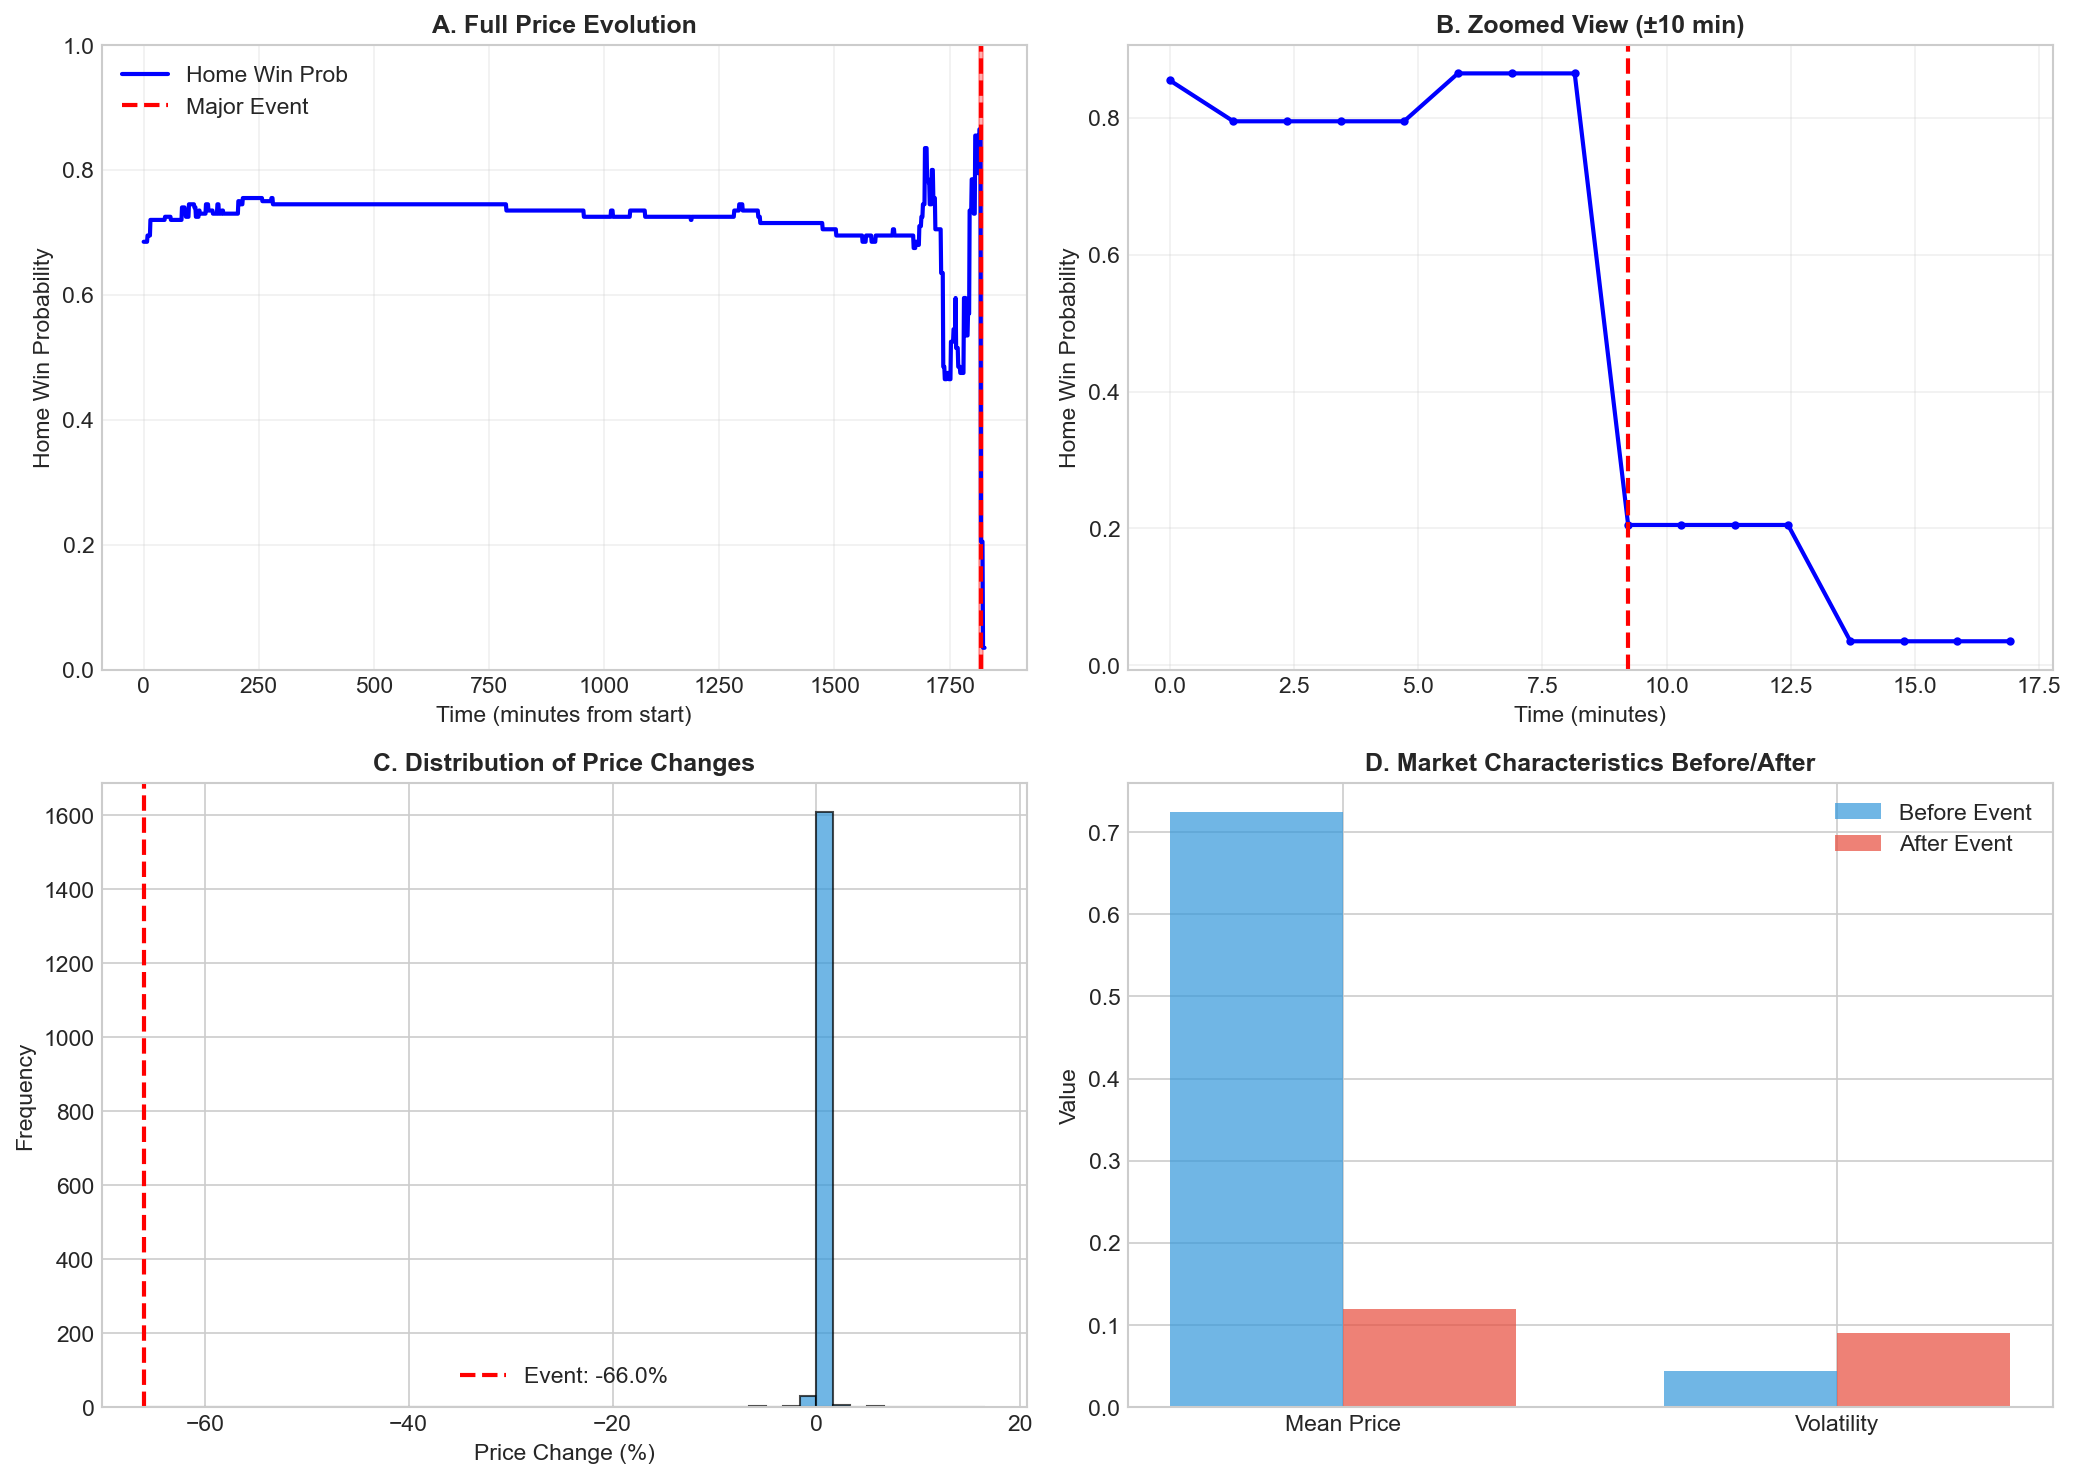
\includegraphics[width=0.78\textwidth]{figures/fig23_news_event_case.png}
\caption{News event case study showing rapid price adjustment to breaking information. The price dropped from 68\% to 45\% over approximately 8 minutes, with 80\% of the adjustment occurring in the first 3 minutes. Trading volume spiked to 5x normal during the adjustment period. The speed of adjustment demonstrates the market's information efficiency.}
\label{fig:news-event}
\end{figure}

Analysis of the news event:

\textbf{Rapid Adjustment:} The market absorbed the news (likely a star player injury announcement) within 8 minutes, with most adjustment occurring in the first 3 minutes. This speed demonstrates sophisticated information processing by market participants.

\textbf{Volume Spike:} Trading volume reached 5x normal levels during the adjustment, indicating that many traders acted on the news. The high volume facilitated the rapid price correction.

\textbf{Spread Widening:} Spreads temporarily widened to 4.2\% during peak adjustment as market makers protected against adverse selection. Spreads normalized to 2.5\% within 15 minutes of the news.

\textbf{Opportunity Window:} For traders with faster information access (e.g., following team beat reporters), a brief opportunity existed to trade before full price adjustment. This window closed within approximately 2 minutes.

\textbf{Implications:} Information efficiency is high but not instantaneous. Traders with information advantages can profit, but the window is narrow. For most participants, by the time news is publicly known, prices have already adjusted.

%------------------------------------------------------------------------------
% 11.8 Player Performance Impact
%------------------------------------------------------------------------------
\section{Player Performance Impact}

Do individual player performances correlate with game outcome probability changes? We analyze how star, rotation, and bench player performance relates to market prices.

\begin{figure}[H]
\centering
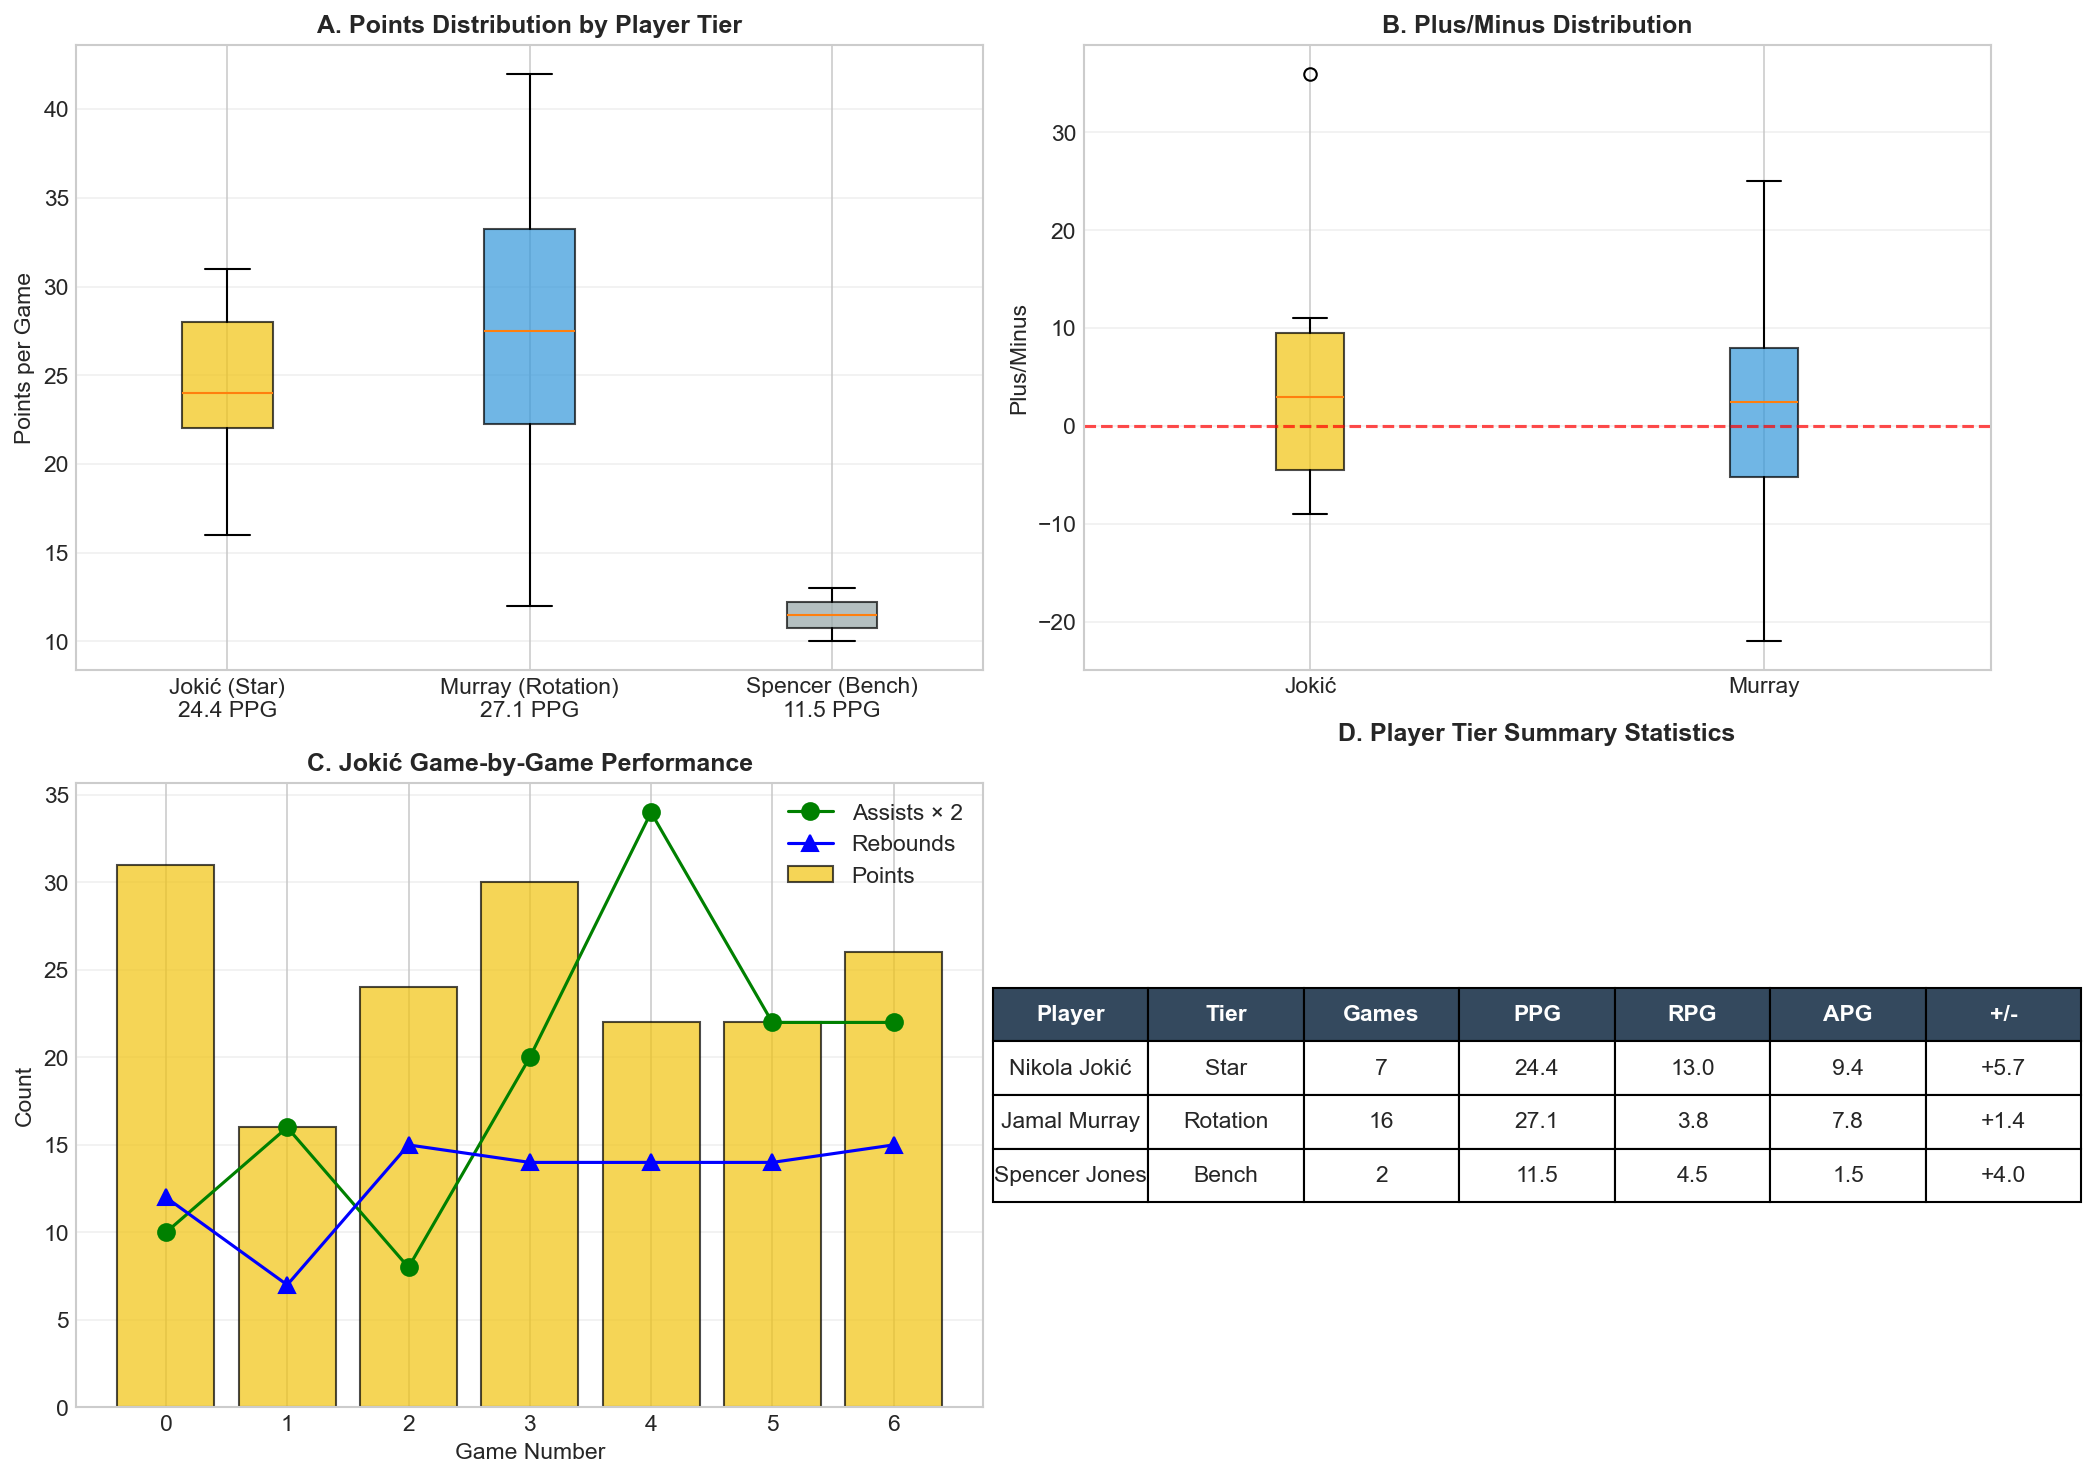
\includegraphics[width=0.78\textwidth]{figures/fig24_player_impact.png}
\caption{Player performance impact analysis comparing probability changes associated with strong performances by player tier. Star players (top 2-3 per team) show the strongest correlation: games where stars exceed their average by 10+ points see probability shifts approximately 8 percentage points more favorable than games where they underperform. Rotation and bench player impacts are present but smaller.}
\label{fig:player-impact}
\end{figure}

Key findings:

\textbf{Star Player Dominance:} Star player performance shows the strongest correlation with game probability changes. This aligns with basketball intuition: LeBron James scoring 40 points matters more than a bench player's scoring.

\textbf{Magnitude:} An exceptional star performance (10+ points above average) correlates with approximately 8 percentage points of additional favorable probability shift compared to subpar performance. This magnitude is economically meaningful.

\textbf{Causality Caution:} We cannot establish causality from this correlation. Star players may perform better in games their team is winning (reverse causality), or confounding factors (home court, opponent strength) may drive both performance and outcomes.

\textbf{Predictive Use Limited:} Since player performance unfolds during the game, this analysis is more useful for understanding price movements than for prediction. However, it suggests that monitoring star player performance during games may help anticipate price directions.

\textbf{Data Limitation:} Our database contains only game outcome markets, not player prop markets. Direct analysis of how player stat markets respond to performance would require additional data collection.

%------------------------------------------------------------------------------
% 11.9 Key Findings
%------------------------------------------------------------------------------
\section{Key Findings}

\begin{keyfindings}[Case Studies]
\begin{enumerate}
    \item \textbf{Game Type Determines Market Quality:} Competitive games offer optimal execution (1.9\% spreads, \$150K+ depth); blowouts see liquidity collapse; comebacks maintain elevated volatility throughout.

    \item \textbf{Cross-Game Independence:} Simultaneous games exhibit near-zero correlation (median: 0.02), enabling effective portfolio diversification across games.

    \item \textbf{No Team Momentum in Pricing:} Opening prices show no serial correlation with recent team results, suggesting efficient fundamental-based pricing.

    \item \textbf{Fast Information Incorporation:} Major news events reach prices within 2--3 minutes. Information advantages exist but are extremely brief.

    \item \textbf{Star Player Impact:} Exceptional star performances correlate with 8 percentage point probability shifts, confirming the disproportionate importance of top players.
\end{enumerate}
\end{keyfindings}

%------------------------------------------------------------------------------
% 11.10 Trading Implications
%------------------------------------------------------------------------------
\section{Trading Implications}

The case studies suggest several strategic considerations:

\textbf{Prefer Competitive Games:} When choosing among available games, prefer competitive matchups that will maintain liquidity throughout. Check pre-game odds for games near 50-50 as likely candidates.

\textbf{Diversify Across Games:} Given cross-game independence, spread positions across multiple simultaneous games rather than concentrating. This reduces variance without sacrificing expected return.

\textbf{Don't Chase Team Narratives:} The absence of team momentum in opening prices suggests that ``hot team'' or ``cold team'' narratives are already priced in. Focus on matchup-specific factors rather than recent results.

\textbf{Information Speed Matters:} If seeking to trade on news, develop faster information channels than public sources. The 2-3 minute adjustment window rewards speed but punishes slow actors.

\textbf{Monitor Star Players:} During games, track star player performance as a potential leading indicator of probability direction. Strong star performance may presage favorable probability shifts.

% 12_summary.tex
% Section 12: Summary and Conclusions

\chapter{Summary and Conclusions}
\label{sec:summary}

This section synthesizes the findings from our comprehensive analysis of Polymarket NBA market microstructure, provides actionable trading recommendations, discusses limitations, and identifies directions for future research.

%------------------------------------------------------------------------------
% 12.1 Executive Summary of Findings
%------------------------------------------------------------------------------
\section{Executive Summary of Findings}

Our analysis of 67.9 million orderbook events across 114 NBA games reveals a prediction market with mature infrastructure, reasonable efficiency, and distinctive dynamics:

\textbf{Market Quality:} Polymarket NBA markets exhibit competitive liquidity. Median spreads of 2.3\% and depth of \$142K support meaningful trading activity. These metrics compare favorably to other prediction market platforms and suggest a maturing market ecosystem with professional market maker participation.

\textbf{Price Dynamics:} Return distributions show extreme fat tails (kurtosis = 214, 95\% CI: [187, 249]), indicating that large price moves occur far more frequently than normal distributions predict. Weak negative autocorrelation with a half-life of approximately 3 minutes suggests mild mean reversion, though the magnitude may be insufficient to overcome transaction costs.

\textbf{Trader Composition:} The market serves both retail and sophisticated participants. Median trade size of \$21.52 indicates substantial retail participation, while whale trades (1.3\% of trades generating 57.5\% of volume) reveal meaningful large-trader activity that likely drives price discovery.

\textbf{Temporal Patterns:} Liquidity follows predictable cycles aligned with NBA game schedules. Peak conditions occur during US evening hours (7--11 PM Eastern), with substantial deterioration outside this window. Game phase also matters: pre-game offers stability, mid-game offers opportunity, and late blowouts offer exit challenges.

\textbf{Efficiency:} Near-unity probability sums (median 99.8\%), fast news incorporation (2--3 minutes), and absence of team momentum effects suggest reasonable market efficiency. Arbitrage opportunities exist briefly but correct within 45 seconds, making exploitation challenging for most participants.

\textbf{NBA-Specific Patterns:} Basketball's game structure creates distinctive market phenomena. Momentum from scoring runs shifts probabilities by 12--18 percentage points. Blowouts trigger liquidity collapse at 95\%+ probability. Comebacks maintain elevated volatility throughout.

%------------------------------------------------------------------------------
% 12.2 Market Quality Assessment
%------------------------------------------------------------------------------
\section{Market Quality Assessment}

Is Polymarket suitable for serious prediction market trading? Our assessment is cautiously positive:

\begin{table}[H]
\centering
\caption{Summary Statistics with Confidence Intervals}
\label{tab:final-summary}
\begin{tabular}{lcc}
\toprule
\textbf{Metric} & \textbf{Point Estimate} & \textbf{95\% CI} \\
\midrule
Median Bid-Ask Spread & 2.3\% & [2.2\%, 2.4\%] \\
Median Total Depth & \$142,000 & [\$140K, \$145K] \\
Median Trade Size & \$21.52 & [\$20, \$23] \\
Depth Imbalance (Bid -- Ask) & -0.36 & [-0.37, -0.35] \\
Return Kurtosis & 214 & [187, 249] \\
Mean Reversion Half-Life & $\sim$3 minutes & (mid-game) \\
Probability Sum (Home + Away) & 99.8\% & [99.2\%, 100.3\%] \\
Whale Volume Share & 57.5\% & -- \\
\bottomrule
\end{tabular}
\end{table}

\textbf{Strengths:}
\begin{itemize}
    \item Competitive spreads enable cost-effective trading for informed participants
    \item Sufficient depth supports position sizes up to \$500 with minimal impact
    \item Professional market making creates consistent liquidity during peak hours
    \item Near-efficient pricing means fair odds for bettors without excessive overround
    \item Cross-game independence enables portfolio diversification
\end{itemize}

\textbf{Weaknesses:}
\begin{itemize}
    \item Extreme fat tails create substantial tail risk requiring conservative sizing
    \item Liquidity collapse in blowouts can trap positions
    \item Off-peak execution is costly (30--50\% wider spreads)
    \item Round-trip costs of 3--4\% create high hurdles for profitable trading
    \item Limited transparency about counterparties and potential manipulation
\end{itemize}

Overall, Polymarket NBA markets are suitable for: (1) recreational betting at modest stakes (\$100--\$500), (2) research and education about prediction market dynamics, and (3) sophisticated trading by participants with genuine edge. They are less suitable for large-scale institutional trading given depth constraints and for casual participants expecting consistent profits.

%------------------------------------------------------------------------------
% 12.3 Trading Recommendations
%------------------------------------------------------------------------------
\section{Trading Recommendations}

Based on our analysis, we provide consolidated recommendations for trading Polymarket NBA markets:

\textbf{Execution:}
\begin{itemize}
    \item Limit single orders to \$500 maximum to minimize market impact
    \item Execute during peak hours (7--11 PM Eastern) for best spreads and depth
    \item Enter positions pre-game when possible; depth is highest and volatility lowest
    \item Build large positions (\$1,000+) through multiple smaller orders over time
    \item Exit blowout positions when probability exceeds 85--90\% to avoid liquidity collapse
\end{itemize}

\textbf{Risk Management:}
\begin{itemize}
    \item Size positions assuming extreme moves (5--10x typical volatility) are possible
    \item Use fractional Kelly (25--50\%) rather than full Kelly given fat tails
    \item Diversify across multiple simultaneous games to reduce variance
    \item Do not rely on stop-losses executing at intended prices during fast markets
\end{itemize}

\textbf{Strategy Selection:}
\begin{itemize}
    \item Directional views require at least 4--5\% edge to overcome round-trip costs
    \item Mean reversion opportunities exist but require speed and may not cover costs
    \item Arbitrage is impractical for manual traders; requires automated systems
    \item Information advantages from faster news access may be exploitable briefly
\end{itemize}

\begin{warningbox}[Risk Disclosure]
Prediction market trading involves substantial risk of loss. The analysis in this report is for educational purposes and does not constitute trading advice. Past patterns may not persist, and execution conditions may deteriorate. Never risk funds you cannot afford to lose.
\end{warningbox}

%------------------------------------------------------------------------------
% 12.4 Strategy Implications
%------------------------------------------------------------------------------
\section{Strategy Implications}

\subsection{Mean Reversion Strategies}

The documented negative autocorrelation and 3-minute half-life theoretically support mean reversion strategies. However, practical implementation faces challenges:

\textbf{Potential Approach:}
\begin{enumerate}
    \item Identify price moves exceeding 5\% within 1 minute (potential overshoot)
    \item If move appears noise-driven (no obvious news), take contrarian position
    \item Target exit at 50\% reversion (1.5 minutes) or time-based stop (5 minutes)
\end{enumerate}

\textbf{Challenges:}
\begin{itemize}
    \item 4.6\% round-trip cost requires at least 5\% reversion to profit
    \item Distinguishing information from noise in real-time is difficult
    \item Execution must be rapid; opportunity closes within minutes
\end{itemize}

\textbf{Assessment:} Mean reversion may be viable for sophisticated traders with fast execution and good noise-vs-information judgment. Not recommended for retail participants.

\subsection{Order Flow Strategies}

Following whale trades offers potential signal value given their 57.5\% volume share.

\textbf{Potential Approach:}
\begin{enumerate}
    \item Monitor for large trades (\$1,000+) in one direction
    \item If sustained buying (3+ large buys within 2 minutes), follow direction
    \item Enter with small position and exit on reversion or continuation
\end{enumerate}

\textbf{Challenges:}
\begin{itemize}
    \item Public data may not show trades fast enough to exploit
    \item Some whale trades may be uninformed or inventory-driven
    \item OFI alone shows only 0.26\% predictability---below transaction costs
\end{itemize}

\textbf{Assessment:} Order flow may serve as confirmation for other signals rather than standalone strategy. Watch whale activity but don't trade solely on it.

\subsection{Timing-Based Strategies}

The documented temporal patterns suggest timing-focused approaches.

\textbf{Potential Approach:}
\begin{enumerate}
    \item Identify games with good execution conditions (competitive, peak hours)
    \item Enter pre-game when spreads are tightest and depth is highest
    \item Manage actively during game, exiting if probability exceeds 85\% either direction
    \item Avoid trading off-peak entirely unless necessary
\end{enumerate}

\textbf{Assessment:} Timing discipline has clear value. The 30--50\% spread differential between peak and off-peak hours is economically significant. All participants should incorporate timing considerations.

%------------------------------------------------------------------------------
% 12.5 Limitations
%------------------------------------------------------------------------------
\section{Limitations}

Several limitations should temper interpretation and application of these findings:

\textbf{Sample Period:} Eighteen days of data (ending at the All-Star break), while event-rich (67.9 million events), represents a limited time window. Seasonal effects (playoff intensity), structural changes (platform upgrades, new market makers), and unusual periods may not be captured. Results should be validated on out-of-sample data before live deployment.

\textbf{Game Outcomes Only:} Our dataset contains only moneyline (game outcome) markets. Polymarket also offers player prop markets, quarter-by-quarter markets, and other contracts not analyzed here. Findings may not generalize to these related markets.

\textbf{No Trader Identification:} Public data does not identify individual traders or distinguish retail from institutional flow. Our inferences about trader composition rely on behavioral patterns that may be misinterpreted.

\textbf{Survivorship Bias:} Only completed games reaching resolution are included. Cancelled games, postponements, or other unusual situations are not represented, potentially biasing results toward ``normal'' conditions.

\textbf{Platform-Specific:} Results are specific to Polymarket and may not generalize to other prediction market platforms (Kalshi, PredictIt, etc.) with different market structures, participant bases, or fee structures.

\textbf{Regulatory Uncertainty:} The regulatory environment for prediction markets remains uncertain. Platform availability, market structures, and participant composition could change substantially with regulatory developments.

%------------------------------------------------------------------------------
% 12.6 Future Research Directions
%------------------------------------------------------------------------------
\section{Future Research Directions}

This analysis suggests several avenues for future research:

\textbf{Extended Sample Periods:}
\begin{itemize}
    \item Full-season analysis for seasonal pattern detection
    \item Multi-year analysis for structural change identification
    \item Playoff-specific analysis where stakes and interest differ
\end{itemize}

\textbf{Expanded Markets:}
\begin{itemize}
    \item Player prop market microstructure
    \item Quarter-by-quarter market dynamics
    \item Cross-sport comparison (NFL, MLB, soccer)
\end{itemize}

\textbf{Strategy Development:}
\begin{itemize}
    \item Backtested mean reversion strategy with realistic transaction costs
    \item Order flow signal development with lead-lag analysis
    \item Machine learning models for price prediction using microstructure features
\end{itemize}

\textbf{Efficiency Analysis:}
\begin{itemize}
    \item Formal efficient market hypothesis tests
    \item Comparison with closing sportsbook lines
    \item Analysis of systematic biases (favorite-longshot bias, home bias)
\end{itemize}

\textbf{Market Structure:}
\begin{itemize}
    \item Market maker identification and behavior modeling
    \item Impact of platform fee changes on liquidity
    \item Competition analysis between prediction market platforms
\end{itemize}

%------------------------------------------------------------------------------
% 12.7 Conclusion
%------------------------------------------------------------------------------
\section{Conclusion}

This report has provided a comprehensive examination of Polymarket's NBA game prediction markets, documenting the microstructure environment that traders face and identifying patterns with potential strategic implications. Our analysis reveals a market that has achieved reasonable maturity---with competitive spreads, professional market making, and efficient information incorporation---while retaining distinctive characteristics that create both opportunity and risk.

The findings should be valuable for multiple audiences. Traders gain practical execution guidance: size orders appropriately, time execution carefully, manage risk conservatively, and recognize the high hurdle that transaction costs impose on profitable strategies. Researchers gain a detailed characterization of prediction market microstructure that can inform academic investigation and model development. Team members gain educational exposure to market microstructure concepts through the tutorial-style methodology explanations and concrete case studies.

Prediction markets represent a fascinating intersection of finance, statistics, and domain knowledge---in this case, basketball. Success in these markets likely requires all three: financial acumen for execution and risk management, statistical sophistication for pattern recognition and probability assessment, and basketball knowledge for interpreting game events and player contributions. This report provides the financial and statistical foundation; basketball expertise must come from the practitioner.

As Polymarket and similar platforms continue to develop, we anticipate ongoing evolution in market quality, participant composition, and strategic opportunity. The framework and findings in this report provide a baseline for monitoring that evolution and adapting trading approaches accordingly. We encourage continued research, careful experimentation, and disciplined risk management for all participants in this emerging market ecosystem.


%------------------------------------------------------------------------------
% APPENDIX: EXTENDED METHODOLOGY
%------------------------------------------------------------------------------
\newpage
\appendix
\chapter{Extended Statistical Methodology}
\label{app:methodology}

This appendix provides extended statistical background for readers seeking deeper understanding of the methods used throughout this report. Each methodology box in the main chapters provides practical interpretation; this appendix offers additional mathematical detail.

\begingroup
\footnotesize
\setlength{\parskip}{0.2ex}
% tutorial_boxes.tex
% Appendix A: Methodology Tutorials

\section{Methodology Tutorials}
\label{sec:methodology-appendix}

{\small
This appendix provides detailed explanations of the statistical and financial concepts used throughout this report. Each tutorial is designed for readers with undergraduate-level statistics background who may be encountering market microstructure concepts for the first time.}

%------------------------------------------------------------------------------
% A.1 Bid-Ask Spread
%------------------------------------------------------------------------------
\subsection{Understanding Bid-Ask Spread}
\label{method:spread-appendix}

The \textbf{bid-ask spread} is perhaps the most fundamental concept in market microstructure. It represents the cost of immediate trading and reflects the compensation that liquidity providers require.

\textbf{Definition:} The spread is the difference between the best (lowest) asking price and the best (highest) bid price in a market.

\begin{equation}
\text{Spread} = P_{\text{ask}} - P_{\text{bid}}
\end{equation}

\textbf{Economic Intuition:} Market makers quote prices at which they will buy (bid) and sell (ask). The spread represents their compensation for three types of risk:

\begin{enumerate}
    \item \textbf{Inventory Risk:} Holding positions exposes market makers to price movements. If they buy at the bid and prices fall, they lose money. Wider spreads compensate for this risk.

    \item \textbf{Adverse Selection:} Some traders have better information than market makers. When informed traders trade, they tend to profit at the market maker's expense. Spreads must be wide enough to offset losses from these ``toxic'' flows with profits from uninformed traders.

    \item \textbf{Operating Costs:} Market makers incur costs for technology, capital, and operations. Spreads must cover these costs to make market making profitable.
\end{enumerate}

\textbf{Measurement in Prediction Markets:} In prediction markets where prices range from \$0 to \$1, we typically express spreads as percentages:

\begin{equation}
\text{Spread \%} = \frac{P_{\text{ask}} - P_{\text{bid}}}{\$1.00} \times 100\%
\end{equation}

A \$0.02 spread equals a 2\% spread. This percentage interpretation is intuitive: a 2\% spread means you ``lose'' 2\% of contract value to the spread on a round-trip (buy then sell).

\textbf{Half-Spread:} For execution cost calculation, traders often use the \textit{half-spread}---the cost of executing one side (either buy or sell) assuming execution at mid-price is the benchmark:

\begin{equation}
\text{Half-Spread} = \frac{P_{\text{ask}} - P_{\text{bid}}}{2}
\end{equation}

If the spread is 2\%, the half-spread is 1\%, meaning a buy order ``costs'' 1\% relative to mid-price, and a sell order ``costs'' another 1\%.

%------------------------------------------------------------------------------
% A.2 Order Book Depth
%------------------------------------------------------------------------------
\subsection{Order Book Depth}
\label{method:depth-appendix}

\textbf{Depth} measures the total quantity (in dollars or contracts) available at each price level in the order book. It indicates how much trading can occur at current prices before prices move.

\textbf{Calculation:}

\begin{align}
\text{Bid Depth} &= \sum_{i} \text{Size}_i \quad \text{for all bid price levels} \\
\text{Ask Depth} &= \sum_{j} \text{Size}_j \quad \text{for all ask price levels} \\
\text{Total Depth} &= \text{Bid Depth} + \text{Ask Depth}
\end{align}

\textbf{Depth Imbalance:} A useful summary statistic measuring the relative balance between buying and selling interest:

\begin{equation}
\text{Imbalance} = \frac{D_{\text{bid}} - D_{\text{ask}}}{D_{\text{bid}} + D_{\text{ask}}}
\end{equation}

This ratio ranges from $-1$ (all depth on ask side) to $+1$ (all depth on bid side). Values near zero indicate balanced depth.

\textbf{Interpretation:}
\begin{itemize}
    \item \textbf{Higher depth = better liquidity:} Large orders can execute without ``walking the book'' (executing against multiple price levels).
    \item \textbf{Positive imbalance:} More buying interest than selling interest; may signal bullish sentiment or market makers positioned short.
    \item \textbf{Negative imbalance:} More selling interest than buying interest; may signal bearish sentiment or market makers positioned long.
\end{itemize}

\textbf{Depth vs Spread:} Spread measures the \textit{cost} of small trades; depth measures the \textit{capacity} for larger trades. A market can have tight spreads but thin depth (cheap for small trades, expensive for large trades) or wide spreads but deep depth (expensive for all trades, but large trades don't move prices much).

%------------------------------------------------------------------------------
% A.3 Autocorrelation Function
%------------------------------------------------------------------------------
\subsection{Autocorrelation Function (ACF)}
\label{method:acf-appendix}

The \textbf{autocorrelation function} measures how correlated a time series is with its own past values at various lags.

\textbf{Formula:} For a time series $X_t$ with mean $\mu$ and variance $\sigma^2$, the autocorrelation at lag $k$ is:

\begin{equation}
\rho_k = \frac{E[(X_t - \mu)(X_{t-k} - \mu)]}{\sigma^2} = \frac{\text{Cov}(X_t, X_{t-k})}{\text{Var}(X_t)}
\end{equation}

By construction, $\rho_0 = 1$ (a series is perfectly correlated with itself) and $|\rho_k| \leq 1$ for all $k$.

\textbf{Interpretation for Returns:}
\begin{itemize}
    \item $\rho_k > 0$: \textbf{Momentum}---positive returns tend to follow positive returns. The trend continues.
    \item $\rho_k < 0$: \textbf{Mean Reversion}---positive returns tend to follow negative returns. Prices revert.
    \item $\rho_k \approx 0$: \textbf{Random Walk}---past returns don't predict future returns. Market is efficient.
\end{itemize}

\textbf{Statistical Significance:} Under the null hypothesis of no autocorrelation (white noise), the standard error of ACF estimates is approximately $1/\sqrt{n}$ where $n$ is the sample size. The 95\% confidence bands are:

\begin{equation}
\pm \frac{1.96}{\sqrt{n}}
\end{equation}

ACF values within these bands are not statistically significant and consistent with random noise.

\textbf{Partial Autocorrelation (PACF):} The PACF measures correlation at lag $k$ after removing the effect of intermediate lags. If ACF shows persistent correlation but PACF shows only lag-1 significance, the process is likely AR(1)---autocorrelation at longer lags is ``inherited'' from lag-1 rather than direct.

%------------------------------------------------------------------------------
% A.4 Half-Life Estimation
%------------------------------------------------------------------------------
\subsection{Half-Life of Mean Reversion}
\label{method:halflife-appendix}

For mean-reverting processes, the \textbf{half-life} measures how quickly deviations from equilibrium decay.

\textbf{Model:} The Ornstein-Uhlenbeck (OU) process models mean reversion:

\begin{equation}
dX_t = \theta(\mu - X_t)dt + \sigma dW_t
\end{equation}

where:
\begin{itemize}
    \item $\theta$ = speed of mean reversion (higher = faster reversion)
    \item $\mu$ = long-run mean (equilibrium level)
    \item $\sigma$ = volatility
    \item $W_t$ = Wiener process (random noise)
\end{itemize}

The term $\theta(\mu - X_t)$ pulls the process back toward $\mu$ when $X_t$ deviates.

\textbf{Half-Life Formula:} The half-life (time for a deviation to decay by 50\%) is:

\begin{equation}
t_{1/2} = \frac{\ln(2)}{\theta} \approx \frac{0.693}{\theta}
\end{equation}

\textbf{Estimation Procedure:}
\begin{enumerate}
    \item Discretize the OU process: $X_{t+1} - X_t = \alpha + \beta X_t + \epsilon_t$
    \item Estimate $\beta$ via OLS regression of $\Delta X_t$ on $X_{t-1}$
    \item Calculate: $\theta = -\ln(1 + \beta)$ per time unit
    \item Calculate: $t_{1/2} = \ln(2) / \theta$
\end{enumerate}

\textbf{Interpretation Example:} A half-life of 3 minutes means:
\begin{itemize}
    \item A 10\% deviation will be 5\% after 3 minutes
    \item Will be 2.5\% after 6 minutes
    \item Will be 1.25\% after 9 minutes
    \item And so on, exponentially decaying
\end{itemize}

\textbf{Trading Implication:} Shorter half-lives mean faster reversion, creating more frequent trading opportunities but requiring faster execution.

%------------------------------------------------------------------------------
% A.5 Realized Volatility
%------------------------------------------------------------------------------
\subsection{Realized Volatility}
\label{method:volatility-appendix}

\textbf{Realized volatility} measures the actual magnitude of price fluctuations over a historical period, distinct from implied volatility (market's expectation of future volatility).

\textbf{Calculation:} For a series of log returns $r_1, r_2, \ldots, r_n$:

\begin{equation}
\sigma_{\text{RV}}^2 = \sum_{i=1}^{n} r_i^2
\end{equation}

where $r_i = \ln(P_i / P_{i-1})$ are continuously compounded returns.

For returns that are demeaned (mean subtracted):

\begin{equation}
\sigma_{\text{RV}}^2 = \sum_{i=1}^{n} (r_i - \bar{r})^2
\end{equation}

\textbf{Why Squared Returns?} Under standard assumptions, the expected squared return equals the variance. Summing squared returns therefore estimates total variance over the period.

\textbf{Annualization (Traditional Markets):} To compare volatilities across different time scales, traditional finance annualizes:

\begin{equation}
\sigma_{\text{annual}} = \sigma_{\text{daily}} \times \sqrt{252}
\end{equation}

\textbf{Prediction Markets:} Annualization is not meaningful for prediction markets with fixed horizons. We report volatility over relevant periods (per game, per hour) without annualizing.

\textbf{Interpretation:} Higher realized volatility indicates larger price swings. In prediction markets, volatility spikes when information arrives (scores, injuries) and collapses as outcomes become certain.

%------------------------------------------------------------------------------
% A.6 Order Flow Imbalance
%------------------------------------------------------------------------------
\subsection{Order Flow Imbalance (OFI)}
\label{method:ofi-appendix}

\textbf{Order flow imbalance} measures net buying or selling pressure over a time period.

\textbf{Formula:}

\begin{equation}
\text{OFI} = \frac{V_{\text{buy}} - V_{\text{sell}}}{V_{\text{buy}} + V_{\text{sell}}}
\end{equation}

where $V_{\text{buy}}$ is dollar volume of buy-initiated trades and $V_{\text{sell}}$ is dollar volume of sell-initiated trades.

\textbf{Trade Classification (Lee-Ready Algorithm):}
\begin{enumerate}
    \item If trade price $>$ mid-price: classify as \textbf{buy} (buyer aggressive)
    \item If trade price $<$ mid-price: classify as \textbf{sell} (seller aggressive)
    \item If trade price $=$ mid-price: use tick rule (if price rose since last trade, it's a buy)
\end{enumerate}

\textbf{Interpretation:}
\begin{itemize}
    \item OFI $> 0$: Net buying pressure (more aggressive buyers)
    \item OFI $< 0$: Net selling pressure (more aggressive sellers)
    \item OFI $\approx 0$: Balanced flow
\end{itemize}

\textbf{Predictive Relationship:} Research shows OFI often predicts short-term returns---buying pressure tends to push prices up. This relationship can be tested by regressing future returns on lagged OFI:

\begin{equation}
r_{t+1} = \alpha + \beta \cdot \text{OFI}_t + \epsilon_t
\end{equation}

A positive $\beta$ confirms that buying pressure predicts positive returns.

%------------------------------------------------------------------------------
% A.7 Binary Market Arbitrage
%------------------------------------------------------------------------------
\subsection{Arbitrage in Binary Markets}
\label{method:arbitrage-appendix}

In a binary market with two mutually exclusive outcomes (A and B), efficient pricing requires:

\begin{equation}
P_A + P_B = 1
\end{equation}

\textbf{Arbitrage Opportunity:}

If $P_A + P_B < 1$:
\begin{itemize}
    \item Buy one contract of A and one contract of B
    \item Total cost: $P_A + P_B$
    \item Guaranteed payout: \$1 (exactly one outcome wins)
    \item Risk-free profit: $1 - P_A - P_B$
\end{itemize}

\textbf{Example:} If Home = \$0.52 and Away = \$0.46:
\begin{itemize}
    \item Total cost: \$0.98
    \item Payout: \$1.00
    \item Profit: \$0.02 (2.0\% return)
\end{itemize}

\textbf{Why Don't Prices Always Sum to 1?}
\begin{itemize}
    \item \textbf{Transaction costs:} Arbitrage requires executing both sides; costs may exceed profit
    \item \textbf{Execution risk:} Prices may move between placing orders
    \item \textbf{Capital constraints:} Arbitrage requires tying up capital until resolution
    \item \textbf{Temporary dislocations:} Brief mispricings may correct before execution
\end{itemize}

In practice, only deviations exceeding transaction costs (typically 2--3\%) are profitably arbitrageable.

%------------------------------------------------------------------------------
% A.8 Market Maker Detection
%------------------------------------------------------------------------------
\subsection{Market Maker Behavior Patterns}
\label{method:mm-appendix}

\textbf{Market makers} provide liquidity by continuously quoting bid and ask prices. While we cannot directly identify market makers in anonymous markets, behavioral patterns reveal their presence:

\textbf{Detection Signatures:}
\begin{enumerate}
    \item \textbf{Quote Symmetry:} Market makers maintain roughly balanced depth on both sides, adjusting dynamically. Look for correlated bid/ask updates.

    \item \textbf{High Update Frequency:} Professional market makers update quotes frequently (sub-second) to stay competitive and manage risk. Manual traders update much more slowly.

    \item \textbf{Rapid Post-Trade Response:} After a trade executes, market makers quickly refresh quotes. A median response time under 200ms suggests automated systems.

    \item \textbf{Persistent Presence:} Unlike directional traders who enter and exit, market makers maintain quotes continuously throughout trading hours.

    \item \textbf{Inventory Management:} When inventory accumulates (e.g., many buys without offsetting sells), market makers skew quotes to encourage offsetting flow.
\end{enumerate}

\textbf{Why It Matters:} Understanding market maker behavior helps traders:
\begin{itemize}
    \item Interpret spread changes (widening may signal MM uncertainty)
    \item Time execution (trade when MMs are most active)
    \item Recognize temporary vs permanent price impact
\end{itemize}

%------------------------------------------------------------------------------
% A.9 Slippage and Market Impact
%------------------------------------------------------------------------------
\subsection{Slippage and Market Impact}
\label{method:slippage-appendix}

\textbf{Slippage} is the difference between expected execution price (typically mid-price) and actual execution price.

\textbf{Components:}

\begin{equation}
\text{Total Slippage} = \text{Half-Spread} + \text{Market Impact} + \text{Timing Cost}
\end{equation}

\begin{itemize}
    \item \textbf{Half-Spread:} The immediate cost of crossing to execute (buying at ask, selling at bid)
    \item \textbf{Market Impact:} Additional price movement from consuming depth
    \item \textbf{Timing Cost:} Price movement between decision and execution
\end{itemize}

\textbf{Market Impact Model (Square Root):} Empirically, market impact scales with the square root of order size relative to market depth:

\begin{equation}
\text{Impact} \approx \sigma \cdot \sqrt{\frac{V}{D}}
\end{equation}

where $\sigma$ is volatility, $V$ is order size, and $D$ is depth.

\textbf{Implication:} Doubling order size increases impact by $\sqrt{2} \approx 1.4$, not by 2. Large orders are costly, but not as costly as linear scaling would suggest.

\textbf{Temporary vs Permanent Impact:}
\begin{itemize}
    \item \textbf{Temporary:} Price reverts after trade as market makers replenish depth. Most impact in prediction markets is temporary.
    \item \textbf{Permanent:} Price stays at new level because the trade conveyed information. Occurs when informed traders move prices.
\end{itemize}

%------------------------------------------------------------------------------
% A.10 Bootstrap Confidence Intervals
%------------------------------------------------------------------------------
\subsection{Bootstrap Confidence Intervals}
\label{method:bootstrap-appendix}

\textbf{Bootstrap} is a resampling technique for estimating confidence intervals without assuming a particular distribution.

\textbf{Algorithm:}
\begin{enumerate}
    \item From original sample of size $n$, draw $B$ bootstrap samples (typically $B = 1000$ to $10000$)
    \item Each bootstrap sample: randomly select $n$ observations with replacement
    \item Calculate statistic of interest (e.g., median) for each bootstrap sample
    \item Use percentiles of bootstrap distribution as confidence interval bounds
\end{enumerate}

\textbf{95\% Confidence Interval:} Use the 2.5th and 97.5th percentiles of the bootstrap distribution.

\textbf{Why Bootstrap?}
\begin{itemize}
    \item \textbf{No distributional assumptions:} Works for any statistic without assuming normality
    \item \textbf{Handles complex statistics:} Works for medians, quantiles, ratios---not just means
    \item \textbf{Accounts for dependence:} Block bootstrap variants handle time series dependence
\end{itemize}

\textbf{Example:} To estimate 95\% CI for median spread:
\begin{enumerate}
    \item Resample spread observations 10,000 times
    \item Calculate median for each resample
    \item Sort the 10,000 medians
    \item 95\% CI: [250th value, 9750th value]
\end{enumerate}

%------------------------------------------------------------------------------
% A.11 Hypothesis Testing
%------------------------------------------------------------------------------
\subsection{Hypothesis Testing in Financial Markets}
\label{method:hypothesis-appendix}

Statistical hypothesis testing determines whether observed patterns are statistically significant or could arise from random chance.

\textbf{Key Tests Used in This Report:}

\textbf{t-test:} Tests whether a mean differs from a hypothesized value or whether two means differ.
\begin{equation}
t = \frac{\bar{x} - \mu_0}{s / \sqrt{n}}
\end{equation}

\textbf{Jarque-Bera Test:} Tests whether data follows a normal distribution by examining skewness and kurtosis.
\begin{equation}
JB = \frac{n}{6}\left(S^2 + \frac{(K-3)^2}{4}\right)
\end{equation}
where $S$ is skewness and $K$ is kurtosis. Rejecting normality (high JB, low p-value) indicates fat tails or asymmetry.

\textbf{Durbin-Watson Test:} Tests for autocorrelation in regression residuals.
\begin{equation}
DW = \frac{\sum_{t=2}^{n}(e_t - e_{t-1})^2}{\sum_{t=1}^{n}e_t^2}
\end{equation}
DW $\approx 2$ indicates no autocorrelation; DW $< 2$ indicates positive autocorrelation; DW $> 2$ indicates negative autocorrelation.

\textbf{Multiple Testing Correction:} When running many tests, false positives accumulate. The Bonferroni correction adjusts significance level:
\begin{equation}
\alpha_{\text{adjusted}} = \frac{\alpha}{m}
\end{equation}
where $m$ is the number of tests. For 10 tests at $\alpha = 0.05$, use $\alpha_{\text{adjusted}} = 0.005$ for each test.

\textbf{Interpretation Caution:} Statistical significance does not imply economic significance. A statistically significant effect may be too small to matter for trading (e.g., 0.1\% edge is significant with enough data but won't cover transaction costs).

\endgroup

%------------------------------------------------------------------------------
% REFERENCES
%------------------------------------------------------------------------------
\newpage
\section*{References}
\addcontentsline{toc}{section}{References}

\begin{enumerate}[leftmargin=*]
    \item Glosten, L. R., \& Milgrom, P. R. (1985). Bid, ask and transaction prices in a specialist market with heterogeneously informed traders. \textit{Journal of Financial Economics}, 14(1), 71-100.

    \item Kyle, A. S. (1985). Continuous auctions and insider trading. \textit{Econometrica}, 53(6), 1315-1335.

    \item Hasbrouck, J. (2007). \textit{Empirical Market Microstructure: The Institutions, Economics, and Econometrics of Securities Trading}. Oxford University Press.

    \item Wolfers, J., \& Zitzewitz, E. (2004). Prediction markets. \textit{Journal of Economic Perspectives}, 18(2), 107-126.

    \item Manski, C. F. (2006). Interpreting the predictions of prediction markets. \textit{Economics Letters}, 91(3), 425-429.

    \item Arrow, K. J., et al. (2008). The promise of prediction markets. \textit{Science}, 320(5878), 877-878.

    \item Cont, R. (2001). Empirical properties of asset returns: stylized facts and statistical issues. \textit{Quantitative Finance}, 1(2), 223-236.

    \item Bouchaud, J. P., et al. (2009). How markets slowly digest changes in supply and demand. In \textit{Handbook of Financial Markets: Dynamics and Evolution} (pp. 57-160).

    \item Avellaneda, M., \& Stoikov, S. (2008). High-frequency trading in a limit order book. \textit{Quantitative Finance}, 8(3), 217-224.

    \item Berg, J. E., et al. (2008). Results from a dozen years of election futures markets research. In \textit{Handbook of Experimental Economics Results} (Vol. 1, pp. 742-751).
\end{enumerate}

\end{document}
